\documentclass[12pt,pagesize, DIV=10, oneside, headsepline,
titlepage,parskip, headings=small, listof=totoc,
bibliography=totoc,index=totoc, captions=tableheading,
 final, abstract=false]{scrreprt}
\usepackage{times}
\usepackage[bottom=3.0cm,top=3.0cm]{geometry}
\usepackage[onehalfspacing]{setspace}
%\usepackage{lipsum}
\usepackage[acronym,toc]{glossaries}
\usepackage{fontspec}
%\usepackage[french]{babel}
\usepackage{polyglossia}
\setdefaultlanguage{french}
\setotherlanguages{german,english}
\usepackage[font=small,labelformat=parens,labelsep=quad]{caption}
\usepackage[french=guillemets]{csquotes}
\usepackage[
backend=biber,        % compilateur par défaut pour biblatex
autolang=hyphen,
style=authoryear-ibid, %apa
style=apa,
%firstinits=true,
giveninits=true,
maxnames=3,
minnames=1,
maxbibnames=99,
ibidtracker=true,
%ibidpage=true,
dashed=false
]{biblatex}

\DeclareFieldFormat{postnote}{#1}
\addbibresource{bib/main.bib}
\usepackage[autooneside=true]{scrlayer-scrpage}
\usepackage{lastpage}



\setkomafont{pagenumber}{\small}
%\renewcommand\pagemark{{\usekomafont{pagenumber}\thepage

%		\,/\,\pageref{LastPage}}}

\ohead*{\pagemark}
%\cofoot*{\pagemark}
\cofoot*{}


\pagestyle{scrheadings}

\automark[section]{chapter}
%\automark*[section]{}

\usepackage{siunitx}
\setcounter{secnumdepth}{3}
\setcounter{tocdepth}{3}
\usepackage{textcomp}
\usepackage{graphicx}
\usepackage{rotating}
\usepackage{pdfpages}
\usepackage{nomencl}
\usepackage{xcolor}
\usepackage[final]{pdfcomment} % nettre 'final' pour enlever les commentaires
\pdfcommentsetup{opacity=0.4}

\hypersetup{
	colorlinks,
	citecolor=black,
	filecolor=black,
	linkcolor=black,
	urlcolor=black
}
%\usepackage[colorlinks=true, %
%	linkcolor=cyan]{hyperref}

\usepackage{marginnote}

\makeatletter
%%%%%%%%%%%%%%%%%%%%%%%%%%%%%% LyX specific LaTeX commands.
\DeclareFontEncoding{LGR}{}{}
\DeclareRobustCommand{\greektext}{%
  \fontencoding{LGR}\selectfont\def\encodingdefault{LGR}}
\DeclareRobustCommand{\textgreek}[1]{\leavevmode{\greektext #1}}
\ProvideTextCommand{\~}{LGR}[1]{\char126#1}


\@ifundefined{date}{}{\date{}}
\makeatother
\renewcommand*{\partformat}{\partname~\thepart}

\title{Le test de la transformation et de l'amélioration de l'écoute à travers le
  processus musicothérapeutique\\
Ein Gehörtest um die Verwandlung und Verbesserung des Hörchens durch
die Musiktherapie festzustellen}

\author{Valérie Gaillard}


\newglossaryentry{computer}
{
  name=computer,
  description={is a programmable machine that receives input,
               stores and manipulates data, and provides
               output in a useful format}
}

\newglossaryentry{Rorschach}
{
  name=musicothérapie,
  description={test projectif}
}

\newacronym{gcd}{GCD}{Greatest Common Divisor}


\newglossaryentry{rémanence}
{
  name=rémanence,
  description={persistance partielle d'un phénomène après disparition
  de sa cause; spécialement de l'aimantation après retrait de
  l'influence magnétique; rémanence ou persistance des images
  visuelles, auditives, phénomènes sur lesquels sont fondés le cinéma
  et l'audition; l'hystérésis: du grec ``usterein= être en retard'':
  c'est un retard de l'effet sur la cause dans le comportement des
  corps soumis à une action (électrique ou magnétique) croissante ou
  décroissante; on parle de cycle d'hystérésis (phys.).}
}

\makeglossaries
\begin{document}
% to get '&' before the last author in multi-author book
\renewcommand{\finalandcomma}{\&}
%\maketitle
%\title{{*}}

%\maketitle
\begin{titlepage}
 \begin{center}
    {\Large
     Zürcher Hochschule der Künste ZHdK\\
 	en collaboration avec l'Interkantonale Hochschule für
        Heilpädagogik HfH \\
	 Upgrade MAS in Klinische Musiktherapie \\ Master of Advanced Studies en musicothérapie clinique\\}
  \vfill
  {\Huge \emph{Le potentiel du test d'écoute Tomatis\textsuperscript \textregistered  pour la 
  musicothérapie} 
  	\vfill%Essai et réflexions en musicothérapie\\ sur des sujets souffrants de troubles de l'humeur 
  %au moyen d'un test d'écoute}
} \medskip


{\LARGE The Potentiel of the Tomatis\textsuperscript \textregistered Listening Test for  Music Therapy } 
\vfill

{\Large Mémoire pour l'obtention du titre de\\ \medskip
Master of Advanced Studies in Klinische Musiktherapie \\ \smallskip 
présenté par Valérie Gaillard}

{\large Directrice de mémoire : Bettina Kandé-Staehelin}



	 \hfill \\
	 \rule{0mm}{1pt} \hfill
{\large Zürich, novembre  2020}
 \end{center}
\end{titlepage}
 % deja commente
%\part{Méthode}
\clearpage
\begin{abstract}
Se visualiser, se voir, se découvrir à travers le reflet de son écoute.
Situer des sons dans l'espace pour se positionner soi-même. Se situer
dans l'espace sonore.

Ecouter et s'écouter.



La musique influe notre corps tout entier. Elle peut influer également notre écoute et même la modifier. Il existe donc un lien entre musique et écoute et nous pouvons le prouver au moyen d'un test et d'un appareil test spécifique que nous estimons adéquat pour se faire.
Cette étude a pour objet de faire l'hypothèse d'une possible visualisation
de la transformation de l'écoute du patient 
lors d'un traitement en musicothérapie. Nous utiliserons la comparaison graphique de ce test qui nous permettra de synthétiser les différences d'écoutes, sortes de "clichés photographiques" de l'écoute avant et après traitement. Nous aurons deux groupes, un groupe test et un groupe témoin.






Mots-clés : musique- musicothérapie-écoute-son-oreille-test
\end{abstract}

\tableofcontents


%\listoftables
%\chapter{Exemple de l'utilisation du glossaire}

Par exemple si tu utilises
le terme de \gls{musicothérapie} il devra être 
défini par dans le glossaire. Comme ce paragraphe
contient une référence à l'entrée du glossaire son
numéro de page sera affiché à côté de l'entrée.

Il est aussi possible de définir les abréviations ou
acronymes. Par exemple le \acrshort{gcd} (sous sa forme
abrégée), ou longue \acrlong{gcd}, voir complète comme
ici \acrfull{gcd} peuvent être utilisée et améliorer
beaucoup la lisibilité du texte en procurant
toujours les mêmes abréviations.

Une fois que ceci est en place il suffit pour obtenir le glossaire:
\begin{enumerate}
\item lualatex master
\item makeglossaries master
\item lualatex master
\end{enumerate}

Actuellement le titre du glossaire apparaît en anglais. Je n'ai pas
encore cherché à modifier ceci. Détail pour l'instant.

\chapter{Introduction et hypothèse}
\begin{quotation}
\emph{Par le Son, le Silence du Non-Être vient à l'Être. Je suis
la musique que je fais ou écoute. La musique a la capacité d'harmoniser
les composantes d'une entité psychophysique pour qu'il soit ``bien
dans sa peau'' et ``bien dans son âme''}\,\footnote{Jacques Viret, \emph{B. A-BA de la musicothérapie}, \cite{viret:b}.}.
\end{quotation}

\section{Introduction}

L'auteur exerce le métier de musicienne professionnelle et a  choisi de compléter sa formation en devenant musicothérapeute  ainsi que consultante à la méthode Tomatis.  



Elle exerce en cabinet privé et en cliniques psychiatriques. L'utilisation de ces deux axes de thérapies varie et s'adapte selon les lieux de travail. En institution, elle est exclusivement musicothérapeute. En cabinet
privé, elle a la liberté d'utiliser l'une des deux techniques ou de les fusionner.
C'est ainsi qu'à travers chaque cas particulier,
elle a modifié ses techniques de soins, et les ai fait évoluer, animée par beaucoup de curiosité! Se lancer dans cette écriture, c'est creuser et approfondir ces recherches. C'est prendre de la distance, observer, se remettre en question, être plus précis dans ses observations, plus systématique dans la manière de travailler. D'où ce questionnement présenté ici : 


\section{Hypothèse: un test pour mesurer les transformations de l'écoute}

L'écoute est-elle universelle ou personnelle ?
 Chaque être humain semble  globalement pareil à un autre; toutes les oreilles paraissent  avoir une anatomie similaire. Et pourtant, si l'on observe de près nos empreintes digitales, on s'aperçoit de l'unicité de chaque être. De même, chaque oreille peut être différente, différenciée et  fonctionner d'une autre façon;  par conséquent notre  écoute pourrait être à chaque fois particulière nous appartenir de façon singulière tout en étant perméable au changement.
Le temps imprime une évolution dans notre être intérieur et extérieur, nous sommes vivants dans nos mouvements psychologiques et physiques. Des traces devraient en être aussi visibles dans l' écoute. Il est plausible de s'en poser la question.
En admettant ainsi qu'il n'y ait pas de statisme mais au contraire une transformation dans l'écoute, ce changement devient identifiable, \textit{remarquable}, unique (dans le sens personnel) à travers nos expériences de vie.  Un test pourrait être un moyen d'évaluer les modifications supposées de cette écoute. 


\subsection{L'hypothèse}

\begin{itemize}
	\item Qu'est-ce qui est proposé ? 
	Utilisation d'un test d'écoute 
	\begin{itemize}
		\item Constat de l'évolution de l'écoute à travers le travail fait en musicothérapie
	\end{itemize}
\end{itemize}


Un test spécifique d'écoute serait  un 
moyen de donner  forme à l'écoute, comme une fenêtre avec une  image, en quelque sorte une \emph{vision de l'écoute}. Avec  des séances de musicothérapie, dont  le son est l'outil, on pourrait en mesurer l'impact sur la façon d'écouter du patient. 

Il  donnerait selon des paramètres de référence, des indices différenciés, propres à chacun sur la perception du son, avec un comparatif en début et fin de thérapie. Il serait  une source d'informations. Il permettrait de visualiser plus objectivement
les changements, la transformation de l'écoute et constater s'il y a un parallélisme dans la transformation psychique  de la personne prise en thérapie.


 L'objet de cette étude est de faire un constat
qui pourrait donner matière à réflexion.
La problématique : 

A cet effet, nous utiliserons un test spécifique à Tomatis, qui se fera dans le cadre d'une musicothérapie. Aucun support de cette méthode n'interviendra, ni \textsl{Oreille
électronique} ni musiques préparées et filtrées. Nous expliquerons la raison de   leur importance mais nous n'en ferons aucun usage. L'idée est de mettre à profit cette forme de test et de  s'en tenir à ce support
graphique, visible, un``dessin'', une image utile, utilisable, tangible,
presque ``palpable'', avec des critères
d'interprétations.


La musicothérapie est une pratique ancestrale. Il suffit de considérer la très grande  place de la musique dans les mythologies et dans les rites.  Selon M. Schneider
\begin{quote}
	elle cherche à sauvegarder et à fortifier la pure substance sonore de l'homme\footnote{M. Schneider, <<\,Le rôle  de la musique dans 
		la mythologie et les rites des civilisations non européennes\,>>,
		\cite{schaeffner.ea:histoire}, tome I, Encyclopédie La Pléiade, 1960, pp. 202--203.}.
\end{quote}

La musique, la matière sonore, est utilisée dans le but d'un 
\begin{quote}
	processus thérapeutique, pour entrer en communication avec soi-même et pouvoir ensuite mieux percevoir le monde qui nous
	entoure, communiquer et s'exprimer\footnote{%
		\href{http://www.musictherapy.ch/fr/musicotherapie/quest-ce-que-la-musicotherapie/}{musictherapy.ch}}.
\end{quote}


L'aspect fugace du son, de la musique, de ce médium volatil par
définition, ne pourra apporter, comme en art-thérapie, le
même aspect concret que peuvent témoigner des supports graphiques,
visuels, reflets d'un espace-temps lors d'un travail d'élaboration
psychique d'un patient. Nous gageons et faisons l'hypothèse que l'action et l'impact de la
musicothérapie sur la façon d'entendre pourraient être perçus, d'une certaine façon plus
clairement, \textsl{ objectivés}, comme saisis par l'\oe il de l'objectif d'un appareil
photographique.
Si nous ne sommes pas médecins ni issus d'un milieu scientifique, en tant que musicothérapeute, nous ne pouvons pas prétendre à l'utilisation des outils
 tel que l'IRMfct; en contre-parti, toutes ces recherches en
neurosciences éclairent, appuient et renforcent la crédibilité de l'action
majeure du son sur notre cerveau, via l'oreille, en démontrant ses effets par cet intermédiaire technique visuel.  Emmanuel Bigand, chercheur, professeur de
psychologie cognitive à l'Université de Bourgogne, relève l'aspect
paradoxal de la musique, la complexité de sa structure sonore sans
fonction biologique précise mais faisant réagir fortement l'être
humain.\footnote{\cite{bigand:cerveau}, chap.~3 p.~35, "Vous avez l'oreille musicale".}.  Notre cerveau peut être activé autant par
la musique que par la nourriture ou la drogue. Et pourtant la musique,
qui est un élément artificiel en soi, n'a aucun rôle dans notre survie ni dans
notre nutrition.


\section{Plan du travail}

Dans la première partie, nous aborderons l'aspect théorique : l'écoute, le son, l'oreille, le test d'écoute, les différents tests d'écoute en musicothérapie.  Ensuite, nous expliquerons  la méthode Tomatis
et puis, beaucoup plus en détail, son test d'écoute.

En deuxième partie ce sera l'aspect clinique : les tests d'écoute réalisés  avec deux groupes de patients en parallèle.

Et finalement suivront la vérification de l'hypothèse, les conclusions et interrogations. 
Quelques réflexions autour notre propre expérience en cabinet privé, étayé d'un cas d'étude.




\chapter{Aspects neurophysiologique: son, écoute}


\section{Le son}

Lors d'un concert, si nous pouvions visualiser les sons qui
s'échappent de l'orchestre, ce serait un chatoiement de cercles qui se
répandraient tout autour de nous, comme 
la propagation des
ronds dans l'eau suite à un ébranlement de sa surface.
Les molécules d'air en contact avec la source sonore se déplacent et
créent une vibration. \autocite[p. 183]{bencivelli:pourquoi,}.


Le son peut être déterminé par différents paramètres
physiologiques et psychologiques.
Il est défini très précisément par un ensemble d'unités physiques chiffrées
: les décibels  et les hertz.\footnote{Voir Annexe: Le son et sa
  définition.}




\section{Ecoute, perception des sons et troubles associés}
\paragraph{Ecouter ou entendre : une différence}

La définition du verbe `entendre' et du verbe `écouter' 
\autocite[pp. 361--385]{hachette:dictionnaire} nous paraît opportune
en raison de la confusion courante des deux termes :
\begin{description}
\item[Entendre] c'est  percevoir des sons, saisir par l'ouïe.
\item[Ecouter] a trois sens: 
\begin{enumerate}
	\item prêter l'oreille à; s'appliquer à entendre;
	\item prêter attention à l'avis de quelqu'un, suivre un avis;
	\item \emph{fig} suivre une impulsion,	une inspiration.
\end{enumerate}
\end{description}


Par les sources étymologiques du
terme `écouter' ,
 sa racine sanskrite \emph{ ``avih'' } se traduit par
 \emph{``évidence'' , ``connaissance'', ``discernement''}. Puis, en ancien
 français, ce mot a donné \textit{``oüir''} signifiant aussi bien \textit{``entendre''} ,
\textbf{`` écouter'' } que \textit{``comprendre''}.\footnote{Source:``Etymologie Français latin grec Sanskrit-Google Sites'' }.
 Est-ce la raison
pour laquelle il subsiste toujours un amalgame 
sur le sens de ce verbe?
Selon Didier
Colin \footnote{Didier Colin,2015 ``Interprétez vos rêves''}, cette faculté
permet non seulement d'écouter et de comprendre avec plus d'attention
mais aussi de percevoir des sons et peut même, être doué de
\textit{``clairaudience'}'. 


En définitive, \emph{entendre} est une attitude passive par rapport au monde sonore
qui nous entoure. Nous recevons les sons sans les interpréter et cela
ne demande aucun effort. C'est une action involontaire et non
sélective.

\textit{Entendre} nous spécifie Bernard Auriol, \autocite[p. 2, ch . 1]{auriol:cle}
\begin{quote}
	<<\,suppose un son (physique), une oreille
	pour le capter, un système nerveux pour le recevoir.\,>>
\end{quote} 
Tandis qu'\textit{écouter} 
\begin{quote}
	<<\,est un
	processus actif supposant préférences et répulsions pour tel son ou
	telle séquence sonore.\,>>
\end{quote}


Entendre et écouter sont donc  «\,deux
fonctions essentiellement distinctes bien qu'évoluant apparemment sur
des terrains identiques\,>>
% ancien texte {\textbf{site internet: http: auriol.free.fr} Extrait de l'entretien réalisé par
%	Bernard Auriol avec Alfred Tomatis, 1973.}.
[\dots] avec «\,l'élément conscient, facteur essentiel sur lequel repose toute la
différence entre ces deux activités\,».\autocite[]{tomatis_oreille_1991}
\pdfmargincomment{Pages des 2 citations?}
\begin{quote}
	
	<<[\ldots] \emph{Entendre, c'est en quelque sorte subir
		un son} ou un message qui nous est adressé. \emph{Ecouter, c'est désirer appréhender ce son} ou ce message [\ldots]>>
	\autocite{tomatis:education}.	
\end{quote}

Selon J. Auriol \autocite[18] {auriol:cle} et Tomatis(\autocite[52]
{tomatis:loreille}, l'écoute est un `` éveil auditif''  défini avec au
minimum trois
fréquences simultanées ( dans le sens esthétique). Il s'agit donc d'un phénomène
complexe avec la corrélation d'axes
linéaires (notion temporelle) et verticales (notion spatiale), doublée d'une
dimension psychologique.

En effet, si \enquote{\emph{Je suis la musique que je fais ou écoute}}\autocite{viret:b}, \textbf{écouter} implique 
une conscience pour s'actualiser dans le sujet. \footnote{Voir point
  \ref{jeSuisLaMusique:viret}, p.2 \pageref{jeSuisLaMusique:viret}.}
Elle est une opération 
qui suppose une participation active dans le choix du message
ou dans la sélection d'une voix. Elle  implique la volonté,
\pdfmargincomment[color=green]{Bien!}
permet une forme de décodage: il s'agit d'une capacité.
Dans un milieu sonore important,
 bruyant, comme un café, lorsque nous lisons attentivement, nous faisons abstraction
des bruits environnants; en soi, nous les entendons parfaitement mais nous n'y
prêtons pas attention. Nous parvenons à couper les sons parasites, à nous en abstraire pour
nous concentrer uniquement sur les plus  pertinents, en l'occurrence
ici ceux de notre lecture intérieure.




  En creusant encore la racine du mot `écouter', celle-ci signifirait aussi \emph{partager}; nous
  remarquons alors à juste titre que nous écoutons le plus souvent en
  face de quelqu'un dans le but de dialoguer, d'échanger. Le même
  phénomène se réalise avec un livre qui transmet et partage des
  connaissances. L'écoute permet donc la communication, sous-entend le
  plus souvent la présence d'un être en vis-à-vis et nécessite de la
  concentration. Il faut cette volonté inclue dans celle-ci  pour
  comprendre et rentrer en contact avec la voix de  l'écrivain qui
  chante dans le texte avec celle, intérieure, du lecteur.

  
 \textbf{Ecouter} se base certes sur une stimulation prenant sa source à 
l'extérieur mais devant être \textbf{ intérieurement et intentionnellement
	recherchée}.




      \paragraph{Ecoute musicothérapeutique}
      

Par extrapolation, nous pouvons aussi différencier les différents types d'écoute. D'après Edith Lecourt \autocite[ch. 10 <<\,De l'écoute verbale à l'écoute musicale\,>>, p. 182.]{lecourt:decouvrir}
 on en distingue plusieurs : l'écoute verbale, musicale, plurivocale et multiple.
 L'analyse musicale qui permet la différenciation d'une voix d'un ensemble polyphonique est appelée \emph{plurivocale}. Celle qui est multiple n'est pas analytique  mais 
 \begin{quote}
 	 [\ldots] \textit{ouvre une disponibilité, met en suspens les grilles verbale et musicale} [\ldots] \emph{pour parcourir le vécu sonoro-affectif}\autocite[p. 183]{lecourt:decouvrir}.
 \end{quote}
 Employée en musicothérapie, Edith Lecourt la nomme la technique de la  \emph{communication sonore} qui peut apporter 
 <<\,des ouvertures sur l'analyse des niveaux plus archaïques de l'organisation mentale.\,>>\autocite[p. 154]{lecourt:decouvrir}	
 Par l'expérience musicale en groupe, il peut y avoir un moment particulier, de ``grâce"  nommé ``le concept d'illusion groupale", l'illusion d'une unité absolue, comme un seul corps\autocite{anzieu:groupal} dont parle Didier Anzieu.


 
\emph{Ecouter} implique les notions de \emph{son} et
d'\emph{oreille}. Nous allons dans un premier temps approfondir  la
définition du son dont les caractéristiques physiques seront mis en
annexes et il en sera de même pour l'oreille et les détails
d'anatomie. \footnote{Annexes: Son et Oreille}

\







\paragraph{Ecoute objective ou subjective?}

Nous avons tous,
selon les manuels d'anatomie, la même
oreille, du moins nous pouvons reconnaître une analogie de structure. Nous devrions donc entendre et écouter la même chose
lors d'une même information diffusée tout comme le fait un enregistreur avec un micro. Pourtant il n'y a pas d'écoute \emph{passive}. Chacun n'entend pas de la même manière les mêmes
informations, chacun trie et fait son propre choix selon la fonction
d'écoute élaborée depuis l'enfance. Cette fonction sélectionne très
rapidement les mots pour être intelligible, pour se faire
comprendre. Nous rejoignons l'idée de Tomatis lorsqu'il affirme que
\textit{"L'oreille a un psychisme"} , car tout un chacun entend ce qu'il veut bien
entendre. \autocite{tomatis_oreille_1998} 
Nous transformons notre écoute selon nos attentes.

Allant dans le même sens, cet 
article d'une 
étude franco-américaine scientifique
\autocite{fritz_stradivarius} au sujet des célèbres violons
Stradivarius: faite avec un protocole 
d'écoutes en aveugle avec
des violonistes professionnels et en parallèle avec un public (caché
derrière un rideau), elle démontre que le mythe de la suprématie
de ces instruments extrêmement chers tombe au profit d'instruments
neufs.

Le cerveau 
transforme les informations reçues selon nos attentes et joue un
rôle majeur dans notre perception.
\autocite{lemonde.fr:stradivarius}.
% 
%\footnote{\href{http://www.lemonde.fr/culture/article/2014/04/10/le-stradivarius-detrone-par-les-violons-modernes\_4398681\_3246.html}{LeMonde.fr}.}.
\autocite[p. 43]{roque:lecoute}


 Freud mettait déjà en évidence le phénomène de la
\textbf{sélectivité }comme ``mécanisme de défense''. \footnote{S.Freud,
  Psychologie de la vie quotidienne, 1904}

En est-il de même lorsqu'il s'agit de patients souffrant de dépression
ou de burnout? Sont-ce justement les souffrances dues à des situations
insupportables qui
ordonnent à notre cerveau de se protéger en obscurcissant la
perception sonore?  Ne plus écouter certains
sons permettrait-il en quelque sorte d'échapper à la souffrance et de faire une
pause dans la douleur? Nous avons le droit et c'est un réflexe de
survie que de ne plus vouloir voir une scène affreuse et de détourner
notre regard. Nous pouvons supposer qu'il en est de même pour l'oreille ne voulant plus capter
certains sons.


 \emph{Vouloir voir, c'est viser.}  Vouloir entendre dans le but d'écouter est comparable  à
la visée de l'\oe il lorsque l'on veut collecter une
information. L'\oe il regarde avec la rétine et  vise, sous l'ordre du
cerveau, avec la macula. Dans la même idée, par l'écoute, nous avons
l'oreille et la cochlée (partie interne de l'oreille) qui permet
l'analyse des sons.




 \textbf{ L'audition est la capacité perceptive du système auditif et l'écoute, c'est ce qu'on en fait.}


\section{La perception des sons et l'existence de troubles
  émotionnels}


Conformément à l'idée que l'oreille nécessite d'être sollicitée pour
énergiser le corps et le cerveau en vue d'un épanouissement, la
capture d'un très haut nombre de stimulations par seconde (3G) agit
sur la formation réticulée,\footnote{Déf.: la formation 
réticulée est la partie centrale de la substance grise du tronc cérébral, 
constituée de nombreuses cellules nerveuses qui communiquent entre elles par de 
multiples jonctions appelées synapses.}
comme prouvé par d'incessantes recherches scientifiques actuelles,
confirmant la très grande complexité de notre cerveau.






                

\paragraph{ La dépression et l'audition dans le rapport
  musique-cerveau}

Depuis la plus haute Antiquité,  la reconnaissance de
l'impact de la musique sur l'émotion est actuellement confirmée par
des approches récentes, dont A.Damasio, \footnote {{L'erreur de
    Descartes}, Antonio Damasio, Paris, 
Ed.Odile Jacob, 1997}, qui souligne l'indispensabilité de l'émotion
sur l'intelligence (intelligence émotionnelle et intelligence
cognitive).
En outre, les approches neuro-psychologiques sur les \textit{agnosies
  auditives}\footnote { Peretz
  I. \textit{in} Seron, Baron et Jeannerod \autocite[<<\,Les agnosies auditives\,>>,
  pp. 205--216]{seron.baron.ea:neuropsychologie}},
sur la perception distincte des émotions de la musique \footnote
{Platel H. 2002\autocite[pp. 223--224]{platel_neuropsychology_2002}}, 
sur l'apport de Bigand E. \footnote {Bigand E. ,chercheur, professeur 
de psychologie cognitive à l'Université 2013 \autocite[Voir ch. 3
p. 35, "Vous avez l'oreille musicale"]{bigand:cerveau} } soutenant le
manque de fonction biologique précise de la musique,
et sur la
découverte du rôle mimétique des\textit{ neurones miroir }( ``troisième''
cerveau) de Rizzolati G.,1990, (???), nous permettent de maintenir et
appuyer 
la fonction thérapeutique de la musique.





\textit{On reconnait qu'il y a un aspect paradoxal de la musique : sa structure n'a pas une 
fonction biologique précise, nous fait remarquer Emmanuel Bigand,  chercheur, professeur 
de psychologie cognitive à l'Université 
de Bourgogne; par contre, elle peut nous faire réagir très fort, autant que la nourriture ou la 
drogue. \autocite[Voir ch. 3 p. 35, "Vous avez l'oreille musicale"]{bigand:cerveau}
D'après Isabelle Peretz
\footnote {\autocite[<<\,Les agnosies auditives\,>>, pp. 205--216]{seron.baron.ea:neuropsychologie}}
ainsi que le chercheur français, Hervé Platel,
\autocite[pp. 223--224]{platel_neuropsychology_2002}
 \enquote{le cerveau traite distinctement les aspects perceptifs et émotionnels de la 
 musique}.}

\footnote{"Notre cerveau n'a pas fini de nous étonner", Entretien avec Jean-Michel 
     Oughourlian, pp. 118--119, Ed. Albin Michel, Le Livre de Poche
     2012.}
   

 
Quant au lien entre audition et dépression, d'autres perspectives
récentes mettent en lumière les évaluations de ces dernières comme  l'échelle
d'Hamilton (rechercher notes en bas de page), comme 
les modifications vocales issues de la dépression \footnote{ Maryland
  University, 2004, 168\ieme\ Congrès de la Société
américaine d'acoustique,.\autocite{le_service_metronews}.  } \footnote{https://www.lci.fr/sante/et-si-on-diagnostiquait-la-depression-avec-u
n-test-vocal-sur-smartphone-1562728.html.},
comme les approches de Szabadi (1976), Yowell (1995), Millot and Brand (2001) et 
Canbeyli (2010), tous soulignant l'important lien entre la difficulté
à percevoir certains sons et la présence de troubles émotionnels,
laissant entendre une correspondance sous forme de '' vase communiquant''
entre la perte de reconnaissance de
sons et un état dépressif.
Une autre étude du CNRS, (2009) mentionne l'effet des événements
traumatisants sur l'audition, impliquant des conséquences dépressives:
la double approche groupale (Gr en bonne santé et Gr déprimé avec
troubles de stress post-traumatique) met en lumière la diminution des
seuils auditifs. (cf. test clinique, ch.6 p. 44) où on relève une augmentation de l'activité de la
première et deuxième aire auditive ainsi qu' une diminution significative des
seuils auditifs par voie osseuse (entre
\SIrange{275}{8000}{\Hz} ) et en conduction aérienne (
\SIrange{500}{875}{\Hz} et  \SIrange{2000}{8000}{\Hz}. 

\paragraph{ Rapport entre audition et émission vocale}

En guise de complètement, le rapport entre audition et émission vocale
est enrichi par l'apport de Granier J.P. ( footnote: psych, format. et
consultant Tomatis à Paris, co-auteur de l'étude des seuls auditifs et
dépressifs) qui soutient qu'``Il existe une 
interaction
constante entre le traitement auditif \textbf{et} moteur de la
voix, entre l'information sensorielle \textbf{et} les programmes moteurs impliqués
dans la parole ou le chant.''

Le programme moteur qui a été déclenché
pour la parole permet au cerveau d'effectuer des tentatives d'anticipation
des émissions acoustiques imminentes, comparées à l'information
auditive reçue; cette boucle
auditivo-vocale/ verbale permettra, dans un processus circulaire, un ajustement.



  
\textit{En regard des recherches actuelles, il est possible de considérer la
dépression sous un autre angle . 
Il existe, mais comme musicothérapeute, il peut être intéressant de trouver
des pistes différentes pour tenter de
déterminer un état dépressif.
Du point de vue de l'émission vocale,
les chercheurs de l'université de Maryland en 
2004 ont révélé lors du 168\ieme\ Congrès de la Société
américaine d'acoustique, que les caractéristiques 
vocales se trouvaient modifiées avec des importants changements
neuro-physiologiques provoqués par la
dépression.\autocite{le_service_metronews}.
\footnote{https://www.lci.fr/sante/et-si-on-diagnostiquait-la-depression-avec-u
n-test-vocal-sur-smartphone-1562728.html.}.

Du point de vue auditif, des publications scientifiques
font le lien entre dépression et perception auditive.
(Szabadi, 1976) (Yowell, 1995) (Millot and Brand, 2001)
(Canbeyli, 2010). Il existerait un lien remarquable  entre la \textbf{difficulté à percevoir} certains sons 
et l'existence 
de\textbf{ troubles émotionnels}.
En d'autres termes, il y
aurait un type de vase communiquant très clair entre\textbf{ la perte de reconnaissance de sons et
  un état dépressif}.

La dépression a été mise en relation avec la
modulation sensorielle et notamment la modification auditive telle que
des altérations de l'audition dûes à des événements
traumatisants. }
L'étude  \footnote{``Les seuils auditifs des sons purs 
	sont diminués chez les personnes déprimées avec des
	troubles de stress post-traumatique.'', <<\,Pure-tone auditory 
	thresholds are decreased in depressed people with post-traumatic stress 
disorder\,>>, Journal of Affective disorders. Recherche du CNRS en collaboration
	avec Tomatis Developpement S.A. Auteurs : Stéphanie 
	Aubert-Khalfa; Emmanuelle Reynaud; Myriam El Khoury;
	Olivier Blin - INCM, UMR CNRS 6193, Jean-Pierre Granier -
	TOMATIS DEVELOPPEMENT S.A. Eva-Maria Grosse; Jean-Claude 
	Samuelian - Pôle Psychiatrie Centre, La Conception Hospital.}
       menée en 2009 par des chercheurs du CNRS à Marseille sur deux
groupes, l'un en bonne santé et l'autre,
sur des personnes déprimées avec des troubles de stress
post-traumatique  atteste du 
fait qu'il y ait une\textbf{ diminution des seuils auditifs} dans ce type de
population.\textbf{ Cf. test clinique ch.6, p.44}--- On a constaté une augmentation de l'activité de la
première et deuxième aire auditive et une diminution significative des
seuils auditifs spécifiquement en courbe osseuse entre
\SIrange{275}{8000}{\Hz} et en conduction aérienne entre
\SIrange{500}{875}{\Hz} et  \SIrange{2000}{8000}{\Hz}. ---







Le nombre limité d'études musicothérapeutiques au sujet du \textbf{burnout}
nous invite aux travaux de Sigrist F. ,  parlant de
\textit{Resonanzstörung'} qui relève la connection neuronale directe et significative entre les systèmes auditif et
         limbique, d'où découle une activation émotionnelle et une
         résonance définie comme ``interpersonnelle''\footnote{"\textit{interpersonnelle Resonanz}"F.Siegrist F. Sigrist, médecin
psychiatre, psychologue et musicothérapeute à la Privatklinik
d'Hohewegg, Zürich.\autocite[pp.55--90] {sigrist_burnout_2016}.}.



Sans nous éloigner trop de notre sujet, nous pouvons rappeler
les difficultés observées sur les
\textbf{autistes} et leur capacité d'écoute cérébrale excessive et
incontrôlable investiguées par Harrisson B. et St-Charles, 2017. \footnote{\autocite[Cet ouvrage propose une description unique du TSA
   (trouble du spectre de l'autisme
   pp. 22--23)]{harrisson.st-charles:lautisme} }. Dans ce tableau
 figure un trouble d'intégration sensorielle (TSA), où
 l'hypersensibilité aux sons devient douloureuse quand le flux excessif
 des
 informations empêche le tri,  protégeant ainsi le cerveau d'une surcharge.


Nous constatons ce lien puissant et indissociable  entre l'ouïe donnée
par l'oreille pour entendre et écouter et le cerveau exécutant ce
travail entre la 
parole et l'oreille.








\chapter{Les différentes approches musicothérapeutiques avec épreuves
  et tests}
Avant d'aborder le test d'écoute qui va nous intéresser plus
particulièrement pour notre travail, nous allons faire la différence
entre la définition du test et celle de l'épreuve.
Le test est normé, c'est une épreuve codifiée, numérisée, échelonnée,
statistifiée. On parle du test d'intelligence de Piaget où il y a une
norme et des chiffres. Tandis que l'épreuve est plus globale, plus complexe,
demande plus de matériel, permet de
cataloguer mais n'est pas statistifiée (pas de chiffres).
Selon Doron et Parot, c'est en 1890 que le test (du latin ``testum''
signifiant ``pot de terre'') a été utilisé pour la
première fois. C'est un procédé d'évaluation qualitative ou
typologique des caractéristiques d'une substance, d'un corps et d'une
fonction.
Le test psychologique est une épreuve définie impliquant une tâche à
remplir, identique pour tous les sujets examinés, avec une technique
précise pour l'appréciation du succès ou de l'échec.
L'épreuve (action d'éprouver) est ce qui permet de juger la valeur
d'une idée, d'une qualité intellectuelle ou morale d'une personne.

\section{Définition du test d'écoute et de l'audiogramme}

De manière générale, le test d'écoute se trouve sous la forme verbale,
à caractère  
psychologique mettant principalement l'accent sur la communication
et la capacité d'empathie.

Dans le milieu médical, on le nomme test d'audition ou audiogramme. Il
sert à mesurer les seuils d'audition des sujets, grâce à l'audiomètre. Cet 
appareil français avait été mis au point en 1933. Les Américains
ont repris ces travaux pendant la dernière guerre pour pouvoir dépister
les dommages subis par ceux qui conduisaient des avions ou d'autres
engins similaires bruyants.
  L'audiogramme est une épreuve d'ordre physiologique. Ce test peut faire partie des examens  pratiqués en otologie\footnote{otologie : branche de la médecine
  	qui étudie l'oreille et ses maladies.} pour poser un diagnostic. 
   C'est un examen à partir duquel se
  dessinent les données dénommées étiologiques\footnote{étiologie : étude des causes
  	d'une maladie} pour détecter un trouble de la fonction auditive. Un pronostic pourra définir le mode de thérapie
médicale, chirurgicale, prothétique ou rééducative. La procédure
technique inclut des paramètres et manipulations propres au corps
médical des auscultations O. R. L. et  n'est pas systématique.






\section{Le test d'écoute en musicothérapie}

Les musicothérapeutes ne se lassent pas d'explorer l'alliage du son
 et de la psychologie, et vice
 et versa, les psychanalystes, les psychiatres, les psychologues
 s'intéressent à intégrer le son dans leur travail. Par ce truchement,
 une élaboration est faite, porteuse d'informations différentes que
 celles d'un questionnaire médical. Le son permet de donner un miroir
 psychologique de la personne par un chemin détourné. Avec cette dimension
 musicale, le test d'écoute diffère de certains tests psychologiques usuels
 et fait partie de ce que l'on nomme le \textbf{ bilan
   psycho-musical}. Celui-ci se déroule soit avec l'audition d'\oe uvres
 musicales où les patients répondent à une grille précise de questions
  soit en trois parties, avec un entretien,
 une écoute musicale (partie réceptive) et une production musicale
 (partie active).
Ce bilan permet d'évaluer la disponibilité du sujet pour cette
approche et permet au thérapeute d'évaluer l'intérêt dans ce cas
d'une telle prise en charge.
 On reconnait de plus en plus le rôle éminemment important que joue la musique
 dans les traitements psychiatriques et ce type de test devient
 fréquent dans beaucoup d' établissements. Ils le sont aussi par principe de précaution et
 par souci d'ajuster au plus près une
 musicothérapie.



  
\section{Les musicothérapeutes et leurs différents types de test}
\label{musicothEtpsycho}

	 La musique s'est révélée ainsi être un important support
         d'expérimentation et 
	 R.Benenzon,  Verdeau-Paillès, Edith
         Lecourt et H.Bonny ont su intégrer dans leur pratique l'utilisation du son comme
         élément facilitant l'exploration psychique.
         Ils ont su, chacun à leur manière  élaborer des procédures destinées à faciliter
         l'introspection et la communication.
\footnote{Nous pouvons aussi citer les recherches telles faites avec la reconnaissance de
bruits, de sonorités (G. Boissière), telle autre avec un test rythmique
(C.Holthaus) ou par celui
des réactions aux intervalles musicaux (Savioz PPIT).} 
Dans d'autres approches, comme F.Nevjinsky, B.Auriol, J. Bonhomme
           et A.Tomatis ont ainsi développé leurs propres
           concepts construisant plusieurs types de \emph{bilans musicaux},
           dont voici une brève énumération.
           

          

         

  \subsection{Benenzon Rolando Omar} 
	\textbf{ Buenos Aires, psychiatre et
    musicien argentin, (1939)}
	  \label{benenzon}
	  Dès 1969 il base sa technique 
	  musicothérapeutique sur des concepts 
	  de Jung, mais s'imprégnant de même de Freud, Winnicott (
          1953, concept d'objet transitionnel) \footnote{
          D. W. Winnicott: ``Jeu et réalité'', Gallimard 1975 }
          Watzlawick. \footnote{ Watzlawick Paul, 1921-2007  théoricien dans la théorie de la communication et le constructivisme radical, membre fondateur de l'École de Palo Alto, psychologue, psychothérapeute, psychanalyste jungien et sociologue} 
	  Influencé par les grands  pédagogues musicaux comme
          Willems(1890-1978, conceptions éducatives faisant la liaison
          entre la musique, l'être humain et le cosmos),
          Dalcroze ou Kodaly ainsi que par l'objet sonore (P.Schaeffer
          et C.Sachs), sa définition de musicothérapie comporte  
	  \emph{\textsl{ ``les expressions corporo-sonoro-non
              verbales''}},\autocite{benenzon:musicotherapie}.
 autocite)
	  centrée sur l'\textit{ISO}" (notion
          d'identité sonore). En séance, il n'utilise pas de
          musicothérapie réceptive mais travaille sur la libération de
          la tension énergétique de l'ISO du patient.

        \subsection{Lecourt Edith}
      \textbf{Psychologue clinicienne,
          psychanalyste, musicienne, musicothérapeute, Paris}. Ses recherches
        actuelles portent sur la psychanalyse de groupe, les
        dimensions subjectives du sonore  et l'émotion esthétique en thérapie.
   Tout comme R.Benenzon, E.Lecourt a recherché  la place qu'occupe le sonore dans la vie d'un 
        patient, et on peut supposer que tous les deux aient sans doute perçu l'idée générale et 
        conductrice de \emph{la méthode projective}, 
        en terme 
	    <<\,d'investigation dynamique et holistique de la
            personnalité\,>>.
            Les tests projectifs sont devenus à partir
        de 1939 un des instruments très utilisés en psychologie
        clinique. Ils réunissaient trois épreuves : le test
        d'association de mots de Jung (1904), le test des taches
        d'encre de Rorschach (1920) et le TAT (test d'histoires à
        inventer) de Murray (1935)\autocite[ch.~1, p.~13]{anzieu.chabert:methodes}.

        Selon E. Lecourt,
(2017)\autocite[ch.~3, p.~84]{Les arts-thérapies,Ed.Armand-Colin}
c'est à Jacqueline Verdeau-Paillès que l'on doit le premier bilan
psycho-musical qu'elle a réalisé avec ses patients dans son service
de psychiatrie à Limoux. Durant cette même période, R.
Benenzon a également élaboré un test similaire \autocite{benenzon:musicotherapie}; on peut supposer qu'ils se soient co-influencés. 


	


\subsection{Verdeau-Paillès Jacqueline
}
\textbf{Neuropsychiatre,
  musicothérapeute, Limoux, France, (1924-2010)}

Avec l'intégration du son dans sa pratique psychanalytique, 
Jacqueline Verdeau-Paillès a introduit  à partir de 1985  un test d'audition d'\oe uvres musicales
sous forme réceptive et active pour réaliser
une relation analytique\autocite{verdeau-pailles:bilan}.
Par ce test, on
observe les réactions comportementales, les productions sonores (
instruments et vocales) et verbales. La technique du montage en U qui débute de 3 à 10
morceaux en fondus enchaînés ( sans interruption) de 3 à 4 minutes chacun, selon les
critères de la culture, l'âge, le milieu,
amène progressivement le patient à un état de détente
avec verbalisation dont découle la possibilité 
d'une hypothèse de
travail et d'établir un projet thérapeutique viable ou non.
Un patient de n'importe quel âge peut exprimer plus facilement les
sensations éprouvées tant à l'écoute qu'à la reproduction
instrumentale ou vocale, ce qui permet d'amplifier la palette d'éléments
cliniques et anamnestiques, facilitant ainsi un meilleur approfondissement du
contenu extériosé, activant aussi l'aspect artistique.
\footnote{ La « troisième oreille » et la pensée musicale, édition Fuzeau, Paris, 2005.
Le bilan psycho-musical et la personnalité, édition Fuzeau, Paris, 3e édition revue et augmentée, 2005.
Expression corporelle, musique et psychothérapie, édition Fuzeau,
Paris, 2e édition revue et augmentée, 2006.} 



\subsection{Bonny Helen Lindquist} 

\textbf{ Musicothérapeute,
  musicienne et psychothérapeute, (1921-2010), Kansas, USA)},

a mis au point dans les années 70
une technique particulière, le GIM,<<\,Guided Imagery and Music\,>>
l'imagerie guidée et de la musique. Selon GIM
Trainings \autocite{gim_site} la
musique associée à la thérapie libère par l'émotion et relie le
conscient à l'inconscient.\footnote{\textsl{The Evolution of Guided Imagery and Music}, 
	by Helen Bonny, Ed. by Lisa Summer (2002), p. 7.}
 C'est une forme réceptive de travail
en musicothérapie, avec comme principales influences Carl Rogers*, Abraham Maslow* et Carl Jung; 
elle  consiste en une longue anamnèse avec le
patient qui permettra de cibler le programme de musiques appropriées. 
(des \oe uvres de compositeurs tels Beethoven, Brahms, Debussy,
Mozart, Rachmaninov ou Vivaldi.)






\subsection{ Nevjinsky Fern}
\textbf{Médecin psychanalyste, 
  Paris, maître de Conférence à Rouen}

 La particularité de Nevjinsky est de rajouter le test psycho-musical
 au test projectif de Rorschach (\gls{Rorschach}), (le test de
 Rorschach est qualitatif et quantitatif, (p.578 psychogramme).
 En effet, lors d'une
 Conférence à ce sujet, il confirme cette méthode 
 avec la comparaison des morceaux de musique en association libre avec
 des jeunes de 13 à 16 ans. 
 L'utilisation des sons purs demeure insuffisante : raison pour
 laquelle il favorise l'utilisation d'oeuvres musicales par
 association libre qui enrichit l'expression des fantasmes et des
 souvenirs.
\autocite[Fern Nevjinsky, maître de conférences à l'Université de Rouen, musicien, psycho-analyste. 
``\textit{Comparaison des modalités de projection et d'expression au test de Rorschach et à un test psycho-musical pour des adolescents de 13 à 16 ans}''.]{nevjinsky:adolescence}.  

 Comme nous le verrons plus loin, Tomatis prétend contrairement que ce sont justement les sons purs
qui ont une portée de diagnostic intéressante.

  \subsection{ Bonhomme Jacques } 
  \textbf{Musicien, musicothérapeute,
    Fonsorbes, France}, a été formé par A.Tomatis. Il se sert du même test d'écoute
      que lui et l'enseigne dans son ``Ecole de la voix'' lors des
      formations qu'il donne. Il a étendu cette  forme active de musicothérapie
      spécifiquement avec la voix 
     et a acquis une
      très grande expérience qu'il transmet en   
      faisant référence au lien entre l'écoute, la voix et la vie
      émotionnelle.
      Il nous livre ses 11 clés phonatoires pour refaire circuler dans
      le corps 
      l'émotion par l'expression de la voix qui est révélatrice des bloquages.
``La voix est la
      résultante de la pensée \textbf{résonnante}  et raisonnante''.
     
\footnote{J.Bonhomme, musicothérapeute, formateur 
  	en expression vocale, musicien, auteur de ``La voix énergie,
        instrument de nos émotions''Ed.Dangles, 1999} 

      \subsection{Auriol Bernard}
 
\paragraph{Médecin psychiatre,
   psychothérapeute, Toulouse, France (1938)}
a étendu ses recherches sur le son, \footnote{Médecin psychiatre, psychothérapeute,  a écrit plusieurs ouvrages, dont : \textsl{Le son au subjectif présent}, \textsl{La clef des sons, Éléments de psychosonique}, \textsl{Méditation et
  psychothérapie}.} la psychosonie, 
tout en s'inspirant également des
travaux d'Alfred Tomatis, avec lequel il s'est formé et sur lequel
nous donnerons plus de détails.

Le terme \emph{psychosonique} a été créé en 1991 par Bernard Auriol pour
désigner la discipline qui cherche à évaluer et décrire les effets du
son sur l'être vivant ainsi que les éléments
subjectifs manifestés par l'expression sonore:  la
voix. La psychosonique s'étend aux éléments
symboliques, psychodynamiques, inconscients et subjectifs du processus
d'écoute. En psychanalyse pour lui, ce n'est pas qu'une affaire de
texte et de parole mais il souligne l'importance de la voix porteuse non seulement
d'imaginaire, de symbolisme mais aussi ``la matérialité insaisissable
des vibrations qui empruntent ``selon Lacan...'' les voies mystérieuses de
l'affect proprement auriculaire''.

\autocite[ch. 13]{auriol:cle}

Sa passion pour le son l'a conduit, entr'autres, à mettre au point des tests
d'écoute, inspirés de ceux d'A. Tomatis.




\textbf{Remarque: } 
On relève ainsi l'importance du \textbf{concept de l'impact du son},\footnote{Source : ASSOCIATION AMARC,
  Association de musicothérapie, recherches cliniques et
  applications) } 
lequel favorise l'expression et le développement de la pensée et va
permettre la prise de conscience des processi pathologiques
développés. Car considéré comme un outil non-anxiogène, même si parfois avec des
techniques un peu divergentes (test ou épreuves), le son provoque l'éveil et l'expression
des affects qui seront à leur tour recueillis dans le bilan psycho-musical.



\subsection{EBQ (Einschätzung Beziehungs Qualität)}
de \textbf{Kathrin Schumacher, Claudine Calvet et Silke Rainer (2011)}


Il existe une autre forme d'estimation de la qualité relationnelle
utile lors de certaines pathologies comme l'autisme pour trouver des
points de repères lors d'une musicothérapie: il s'agit d'un instrument d'évaluation relationnelle entre patient et
thérapeute fournissant à ce dernier des éléments de soutien pour le
processus. Il est alors possible de retenir les étapes présentées dans une étude de cas
((KEBQ,UBQ,IBQ) MAS Novembre 2018,
Barbara ...) observées au stade pré-verbal, verbal et dans les expressions
émotivo-corporelles.
Dans une phase ultérieure, le travail se focalise sur l'estimation de
la stimulation en vue d'une intervention bénéfique et plus
satisfaisante avec l'application de 7 modes différents, numérisables
et comparables entre eux.\footnote{ Auteurs: K.Schumacher,
  Cl.Calvet, S.Reiner,''EBQ und seine Entwicklungspsychologien Grundlagen'' Ed. Vanderhoeck-Ruprecht, 2011 } 




  



  
\subsection{Tomatis Alfred}

\textbf{Médecin spécialiste en neurophysiologie auditive et en
oto-rhino-laryngologie, A. Tomatis, (Marseille 1921-Paris 2001) } fonde
\textit{\textbf{l'audio-psycho-phonologie }} à la Sorbonne entre 
1957 et entre 1960 en  se penchant sur la relation 
\textit{``oreille -- voix''}, et entre la relation \textit{``écoute
et communication''}, publiant plus de douze livres et de nombreux
articles en partie issus de ses
conférences\footnote{cf. Bibliographie}.

Dans le contexte d'étude des troubles de
l'oreille présentés chez des employés de l'aviation militaire
française, il décèle, à l'aide
de tests audiométriques
 (1947), des pertes auditives accompagnées d'une
déformation de la voix associée à des troubles
cognitivo-comportementaux et posturaux.(Cf.plus loin)

Des diagnostiques analogues ont pu être établis dans des situations
de souffrances avec surdité auprès de chanteurs professionnels,
ceci donnant lieu
à un nouveau concept de
\textbf{parallélisme } entre l'examen audiométrique et la courbe
d'enveloppe dans l'analyse des fréquences de la voix.
En effet, le patient ne peut pas reproduire les fréquences qu'il
n'entend pas: 
la perturbation de la voix n'étant pas causée par un défaut des cordes
vocales, mais par une altération de la perception auditive (conduction
sonore osseuse et conduction aérienne), d'où
l'idée d'une correction à l'aide d'un appareil l'Oreille
Electronique, avec ``effet Tomatis'' induisant
une syntonisation de la réponse vocale.

 De plus, les prescriptions habituelles des phoniatres de
l'époque traitant la tension des cordes vocales --au même titre que
l'accordage d'un violon--par le sulfate de
strychnine s'étaient révélées inappropriées.

Dans le schéma ci-dessous est représentée l'Oreille Electronique
comportant deux canaux reliés par une bascule.\footnote{Il existe une étude pilote sur l'effet de 
--- la \textbf{bascule} \label{bascule} électronique, permettant une meilleure
captation des sons ---du Dr. Carlos Escera
de l'Université de Barcelone en 2014, menée en collaboration avec le CNRS.
\href{http://tomatisassociation.org/scientific-validation-of-the-tomatis-effect-
eeg-recordings-of-sound-from-brainstem-to-cerebral-cortex-encoding-university-of
-barcelona-2014/}{tomatisassociation.org}.}  \label{bascule}
 Dès que le sujet (avec
des écouteurs pour un retour modifié de sa voix) parle
dans le micro (M), le canal 1 (C1) se ferme et  le canal 2 (C2) contraint le
système à un autre mode de contrôle.
\typeout{but ultime: l'obtention d'une posture d'auto-écoute favorable à une
          émission vocale de qualité. \autocite[97]{tomatis_oreille_1998}}

\begin{figure}
	\centering
	\includegraphics[width=0.7\linewidth]{images/oreilleelectro.jpg}
	\caption[oreilleelectro]{Schéma initial de l'Oreille
          Electronique}
       
	\label{oreilleelectro}
\end{figure}


      
En fait, ce schéma comprend le\textit{ feed-back}, un des principes
cybernétiques lié au concept de l'\textit{homéostasie} tel
mentonné dans le dictionnaire de psychologie.\autocite[298]{doronparot}\footnote{Doron et Parot, rétroaction;
  feedback positif = il faut varier, f.négatif= ne rien faire,  feed-back, Doron/ Parot, .p177 : cybernétique. Concept de l'homéostasie, Cannon}



 En effet, dès les premières
séances, Tomatis constate une amélioration temporaire de la voix, se
stabilisant avec l'entraînement, et établissant ainsi
\textbf{le lien frappant entre l'écoute et
  l'émission vocale}.

\textbf{L'ensemble de ces considérations préalables nous permettent d'accéder au choix de
cette méthode de testing appliquable à ma recherche.}

%\input{chapitretomatis}
%
\subsection{ 
Le test d' Alfred Tomatis}

\paragraph{Le test d'écoute TSLT: conçu par Tomatis,
   cet appareil, appelé ``\emph{Hearing Test}'', permet de traduire l'écoute par 
   un graphique. La
   qualité de l'écoute est objectivée.}

 
est basé sur des sons purs et leur
 reconnaissance, ce qui permet d'objectiver la qualité de l'écoute; il a été créé dans les années 50, avec un
  appareil contenant un générateur de fréquences qui émet des sons
  purs s'étalant de \SIrange{125}{8000}{\Hz}, d'octave en octave, en passant par les valeurs
\SIlist{1500;3000;6000}{\Hz}, et dont l'intensité, peut varier de 5 en \SI{5}{\dB}, de \SIrange{10}{100}{\dB}. 
Ceux-ci sont transmis au moyen d'une
  transmission aérienne (avec un casque) et osseuse (avec un vibrateur). Ces sons sont à identifier et à
  signaler par le patient en levant la main du côté où il l'entend. On
  varie le volume (de très faible à fort). En procédant de manière
  simple, aucune performance, aucune note à transcrire, n'est demandée
  au patient, ni une 
  recherche de sens ou d'association d'idées.
 
 Détecter un son précis, l'entendre, reconnaitre sa présence et même à très
 faible intensité, le situer dans l'espace, à droite, à gauche, au
 milieu ou ailleurs,  apporte une particularité qui est celle de  donner simultanément  \textbf{une information
   physiologique et psychologique} sur le patient.
 C'est pour cette raison qu'il a été nommé
 audio (oreille)-psycho-phonologique (voix). \footnote{\footnote{Avec le professeur Tomatis: formation suivie dès 1995, Boulevard de Courcelles, Centre de l'écoute 
Tomatis à Paris; puis en 2009/11/13/15 avec V. Gas, V. Drouot et J.P. Granier, formateurs et consultants. Source: site internet officiel: \cite{tomatis.com}.}
.}
  
  Dans son ouvrage \emph{Éducation et
    Dyslexie}\autocite{tomatis:education} il
  a présenté ce test d'écoute comme étant très important car il détermine les
  possibilités d'écoute du sujet : auto-écoute et écoute de
  l'autre\footnote{<<\,Considérations sur le test d'écoute\,>>. Propos
  	recueillis au cours du \textsc{iii}\ieme\ congrès international
  	d'audio-psycho-phonologie (Anvers 1973) à la suite d'un entretien recueilli par B. Auriol
  	avec le professeur Tomatis. \autocite{auriol_stress}.}. 
   Les procédures de passation du test semblent
  se rapprocher d'un audiogramme classique mais il n'en est rien car
  le but d'un audiogramme classique  est de mettre en évidence un
  trouble de l'audition.\footnote{Cf. \ref{passation}, p. 
    \pageref{passation}.}.
  

  On détecte donc si le patient désire ou non se servir des sons
  qu'il a à sa disposition. Il a peut-être la possibilité d'entendre un large spectre de
  sons mais ne souhaite pas, ne veut pas les écouter. Les raisons sont multiples et en général d'ordre psychologique (traumatismes,
  expériences négatives). Le cerveau aura le
  pouvoir d'assourdir certaines fréquences, de les masquer jusqu'à les faire disparaître peu à peu de
  son champ d'écoute. Par protection, par réflexe de survie, le
  patient choisit de les
  annihiler alors que les sons sont là, réels, et que  l'oreille peut physiquement les collecter. Le cerveau crée ce
  que l'on appelle des distorsions
  d'écoute\autocite{tomatis:education}.

  
  Ce test est un test spécifique destiné à fournir une traduction
graphique de l'écoute, et d'en objectiver la qualité. Plus précisément,
il  est fait pour :
\begin{itemize}
\item constater la posture d'écoute de la personne ainsi que de vérifier
la fonction de dynamisation, la fonction vestibulaire,
et la fonction d'écoute.
\item observer les modifications et les évolutions des courbes
  aériennes et osseuses au cours
de la thérapie.
\end{itemize}

Cette mise en évidence des seuils d'écoute est une forme d'objectivité
--- quoique cette notion comme dit précédemment, est très complexe
avec le son ---; mais en un même temps, et cela peut paraître paradoxal, il
est possible d'analyser par ces résultats le potentiel d'écoute de
chaque patient en particulier.




Tomatis a défini la «courbe d'écoute idéale», courbe qui correspond à l'oreille absolue
des chanteurs et des musiciens,  avec  le ténor italien Enrico
Caruso (1873--1921) dont il a analysa la voix à partir des enregistrements
de ses vocalises sur vinyles. Caruso représentait la courbe auditive
optimale dont il décida de se référer.

\begin{figure}
	\centering
	\includegraphics[width=0.7\linewidth]{images/courbeideale.jpg}
	\caption{Courbe idéale}
	\label{fig:courbeideale}
      \end{figure}

      
Sur le plan de la physique pure, elle indique les réponses de l'oreille
lorsque celle-ci fonctionne bien. Elle répond en fait à la courbe
de Wegel dite ``courbe en citron", inversée.\footnote{%
		Voir l'annexe \ref{acoustique} p. \pageref{acoustique}
		 pour cette partie technique.}.

               

L'acquisition de cette courbe idéale correspond à l'\textsl{harmonisation}
du jeu de deux muscles de l'oreille moyenne. Ce jeu
permet de régler en permanence la pression interne au niveau du
labyrinthe.
Lorsque l'interprétation des informations transmises à l'oreille est
erronée, il s'agit donc  de
distorsions d'écoute, déjà citées plus haut. Cette distorsion est liée au dysfonctionnement
de ces deux muscles de l'oreille moyenne dont le rôle est de permettre l'arrivée
harmonieuse du son dans l'oreille interne, puis au cerveau. Car, lorsque
le message sensoriel est altéré, le cerveau se protège en déclenchant
des mécanismes d'inhibition de l'écoute. On naît
avec ce potentiel mais celui-ci s'altère parfois avec les difficultés
de la vie et on introduit des distorsions
pour se défendre contre certaines agressions du monde extérieur. 

Sur le plan du test d'écoute, on remarquera
alors des distorsions, des manques par rapport à la courbe dite 
idéale.
Et lorsqu'il n'y a pas de distorsions, on parle d'harmonie. L'harmonie
est la régulation des émotions, l'équilibre entre son écoute
intérieure et extérieure. On la visualisera sous la forme de
courbes continues et parallèles.
Ces paramètres sont importants et nous reviendrons plus en détail sur le test d'écoute :(8.3.2)
%\enquote{\emph{L'oreille a un
%psychisme\autocite[{tomatis:loreille}.}} 




  




 




  


%\part{Méthode Tomatis}
\chapter{Alfred Tomatis}


\subsection{ 
Le test d' Alfred Tomatis}

\paragraph{Le test d'écoute TSLT: conçu par Tomatis,
   cet appareil, appelé ``\emph{Hearing Test}'', permet de traduire l'écoute par 
   un graphique. La
   qualité de l'écoute est objectivée.}

 
est basé sur des sons purs et leur
 reconnaissance, ce qui permet d'objectiver la qualité de l'écoute; il a été créé dans les années 50, avec un
  appareil contenant un générateur de fréquences qui émet des sons
  purs s'étalant de \SIrange{125}{8000}{\Hz}, d'octave en octave, en passant par les valeurs
\SIlist{1500;3000;6000}{\Hz}, et dont l'intensité, peut varier de 5 en \SI{5}{\dB}, de \SIrange{10}{100}{\dB}. 
Ceux-ci sont transmis au moyen d'une
  transmission aérienne (avec un casque) et osseuse (avec un vibrateur). Ces sons sont à identifier et à
  signaler par le patient en levant la main du côté où il l'entend. On
  varie le volume (de très faible à fort). En procédant de manière
  simple, aucune performance, aucune note à transcrire, n'est demandée
  au patient, ni une 
  recherche de sens ou d'association d'idées.
 
 Détecter un son précis, l'entendre, reconnaitre sa présence et même à très
 faible intensité, le situer dans l'espace, à droite, à gauche, au
 milieu ou ailleurs,  apporte une particularité qui est celle de  donner simultanément  \textbf{une information
   physiologique et psychologique} sur le patient.
 C'est pour cette raison qu'il a été nommé
 audio (oreille)-psycho-phonologique (voix). \footnote{\footnote{Avec le professeur Tomatis: formation suivie dès 1995, Boulevard de Courcelles, Centre de l'écoute 
Tomatis à Paris; puis en 2009/11/13/15 avec V. Gas, V. Drouot et J.P. Granier, formateurs et consultants. Source: site internet officiel: \cite{tomatis.com}.}
.}
  
  Dans son ouvrage \emph{Éducation et
    Dyslexie}\autocite{tomatis:education} il
  a présenté ce test d'écoute comme étant très important car il détermine les
  possibilités d'écoute du sujet : auto-écoute et écoute de
  l'autre\footnote{<<\,Considérations sur le test d'écoute\,>>. Propos
  	recueillis au cours du \textsc{iii}\ieme\ congrès international
  	d'audio-psycho-phonologie (Anvers 1973) à la suite d'un entretien recueilli par B. Auriol
  	avec le professeur Tomatis. \autocite{auriol_stress}.}. 
   Les procédures de passation du test semblent
  se rapprocher d'un audiogramme classique mais il n'en est rien car
  le but d'un audiogramme classique  est de mettre en évidence un
  trouble de l'audition.\footnote{Cf. \ref{passation}, p. 
    \pageref{passation}.}.
  

  On détecte donc si le patient désire ou non se servir des sons
  qu'il a à sa disposition. Il a peut-être la possibilité d'entendre un large spectre de
  sons mais ne souhaite pas, ne veut pas les écouter. Les raisons sont multiples et en général d'ordre psychologique (traumatismes,
  expériences négatives). Le cerveau aura le
  pouvoir d'assourdir certaines fréquences, de les masquer jusqu'à les faire disparaître peu à peu de
  son champ d'écoute. Par protection, par réflexe de survie, le
  patient choisit de les
  annihiler alors que les sons sont là, réels, et que  l'oreille peut physiquement les collecter. Le cerveau crée ce
  que l'on appelle des distorsions
  d'écoute\autocite{tomatis:education}.

  
  Ce test est un test spécifique destiné à fournir une traduction
graphique de l'écoute, et d'en objectiver la qualité. Plus précisément,
il  est fait pour :
\begin{itemize}
\item constater la posture d'écoute de la personne ainsi que de vérifier
la fonction de dynamisation, la fonction vestibulaire,
et la fonction d'écoute.
\item observer les modifications et les évolutions des courbes
  aériennes et osseuses au cours
de la thérapie.
\end{itemize}

Cette mise en évidence des seuils d'écoute est une forme d'objectivité
--- quoique cette notion comme dit précédemment, est très complexe
avec le son ---; mais en un même temps, et cela peut paraître paradoxal, il
est possible d'analyser par ces résultats le potentiel d'écoute de
chaque patient en particulier.




Tomatis a défini la «courbe d'écoute idéale», courbe qui correspond à l'oreille absolue
des chanteurs et des musiciens,  avec  le ténor italien Enrico
Caruso (1873--1921) dont il a analysa la voix à partir des enregistrements
de ses vocalises sur vinyles. Caruso représentait la courbe auditive
optimale dont il décida de se référer.

\begin{figure}
	\centering
	\includegraphics[width=0.7\linewidth]{images/courbeideale.jpg}
	\caption{Courbe idéale}
	\label{fig:courbeideale}
      \end{figure}

      
Sur le plan de la physique pure, elle indique les réponses de l'oreille
lorsque celle-ci fonctionne bien. Elle répond en fait à la courbe
de Wegel dite ``courbe en citron", inversée.\footnote{%
		Voir l'annexe \ref{acoustique} p. \pageref{acoustique}
		 pour cette partie technique.}.

               

L'acquisition de cette courbe idéale correspond à l'\textsl{harmonisation}
du jeu de deux muscles de l'oreille moyenne. Ce jeu
permet de régler en permanence la pression interne au niveau du
labyrinthe.
Lorsque l'interprétation des informations transmises à l'oreille est
erronée, il s'agit donc  de
distorsions d'écoute, déjà citées plus haut. Cette distorsion est liée au dysfonctionnement
de ces deux muscles de l'oreille moyenne dont le rôle est de permettre l'arrivée
harmonieuse du son dans l'oreille interne, puis au cerveau. Car, lorsque
le message sensoriel est altéré, le cerveau se protège en déclenchant
des mécanismes d'inhibition de l'écoute. On naît
avec ce potentiel mais celui-ci s'altère parfois avec les difficultés
de la vie et on introduit des distorsions
pour se défendre contre certaines agressions du monde extérieur. 

Sur le plan du test d'écoute, on remarquera
alors des distorsions, des manques par rapport à la courbe dite 
idéale.
Et lorsqu'il n'y a pas de distorsions, on parle d'harmonie. L'harmonie
est la régulation des émotions, l'équilibre entre son écoute
intérieure et extérieure. On la visualisera sous la forme de
courbes continues et parallèles.
Ces paramètres sont importants et nous reviendrons plus en détail sur le test d'écoute :(8.3.2)
%\enquote{\emph{L'oreille a un
%psychisme\autocite[{tomatis:loreille}.}} 




  




 




  


Pour entrer dans le noyau du thème abordé, nous considérons utile
l'approfondissement de certaines notions.
\section{Méthode et test d'écoute}

Par {\textit{l'audio-psycho-phonologie}}, on entend l'étude des
phénomènes auditifs, phoniques et psychologiques et leurs anomalies.


De ces dernières dérive la mise en place d'un processus pédagogique
et/ou thérapeutique pouvant 
utiliser plusieurs techniques.
Une de ces techniques,
  appelée
\label{outil_oreille_electro}
\textit{Oreille Electronique}, utilise 
un système appelé \textit{ la 
bascule}, permettant de créer une alternance entre deux conditions perceptives 
du même message sonore, avec un passage soudain et imprévu de fréquences graves à des 
fréquences aiguës.


Cette application favorise une amélioration naturelle \emph{d'interprétation du message
sensoriel}, répondant à des objectifs rééducatifs, par ailleurs en
interaction avec la psycho-neuro-immunologie (PNI),
\footnote{La PNI étudie 
l'impact des événements psychiques sur le système immunitaire. Elle repose sur 
la mise en évidence d'interrelations entre le système
nerveux central, le système neuroendocrinien et le système immunitaire.
C'est une approche interdisciplinaire incorporant des données de la
psychologie, de la neuroscience, de la neurologie, dont l'endocrinologie
et l'immunologie. (entre autres) Source : Wikipédia, février 17.}
elle- même sensible à
l'impact des événements psychiques sur le système immunitaire.

Cette
conception intégrative de l'homme met en interaction toutes les
dimensions corporelles et psychologiques, dont les émotions et les cognitions.


``L'effet Tomatis'' est constitué par les principes suivants:  
\begin{itemize}
	\item La voix est soumise à l'oreille, c.à. dire la voix ne contient que ce que l'oreille entend.
	\item Toute modification de l'audition implique immédiatement
          et inconsciemment une
          modification de la voix.
	\item Il est possible de transformer l'émission vocale par une stimulation 
auditive
		entretenue pendant un certain temps (loi de
                ``rémanence'' ). \footnote {persistance partielle d'un phénomène
                après disparition de sa cause; spécialement de
                l'aimantation après retrait de l'influence magnétique;
                rémanence ou persistance des images visuelles, auditives,
                phénomènes sur lesquels sont fondés le cinéma et
                l'audition; l'hystérésis: grec usterein=''être en
                retard'': c'est un retard de l'effet sur la cause dans
                le comportement des corps soumis à une action(
                électrique ou magnétique) croissante, ou décroissante;
                on parle de cycle d'hystérésis ( phys.)}
\end{itemize}

Dans sa globalité, l'``effet Tomatis'' se manifeste par une action
simultanée sur les fonctions de
l'oreille en touchant le système nerveux central (SNC) (coordination
                motrice et l'équilibre), par l'intermédaire du système
                vestibulaire.

                De même, \textit{l'effet Tomatis} agit aussi sur certains troubles
                neurophysiologiques. cf. aussi l'autisme avec Tomatis
                Il joue également un rôle de dynamisation cérébrale et corporelle
               par des fréquences spécifiques.





Il serait important à ce moment d'offrir une vision plus ample de
l'articulation entre l'approche de Bekésy et l'approche de Tomatis,
raison pour laquelle nous mentionnons les différences conceptuelles de
base entre les deux chercheurs.
\paragraph{Les différences conceptuelles de la physiologie auditive
  entre Bekésy et Tomatis}.



En bref, dans  l'approche de von\textbf{ Bekésy} (Budapest 1899-Honolulu 1972,
physicien américain d'origine hongroise) ses
recherches en acoustique concernant les techniques de communication
téléphonique l'amenèrent à s'intéresser au problème de l'audition et à
élaborer des modèles de fonctionnement de l'oreille. Il élucida en
particulier le rôle de la membrane basilaire, et ses découvertes
permirent d'améliorer les traitements de la surdité.  (PN, prix 
Nobel de physiologie 1961).
Sa vision affirme que la fonction principale de l'oreille
consiste à transmettre les sons de manière passive, au même titre qu'un micro et le rôle des osselets 
est limité à sa simple transmission du
son. Il avait déjà énoncé cette loi en 1923, et elle a été adoptée
universellement dans les sciences physiologiques.


En divergence avec G. Békésy, \textbf{Tomatis} oppose la conception de la 
physiologie auditive comme \textbf{active} et non passive.\footnote{Cf. Annexe sur l'anatomie de l'oreille et sa physiologie}
Son originalité réside ainsi dans la transmission du son
au niveau de l'oreille moyenne et interne. Ainsi: 



\begin{itemize}
	\item Le tympan, dans son rôle de transmetteur dans l'oreille
          moyenne, effectue --grâce aux muscles de l'étrier et du marteau--
		un\textbf{ travail de visée} en ciblant les sons. Il 
se tend
		pour se mettre en résonance avec les sons à percevoir
                et fait aussi un autre travail qui est celui de \textbf{sélectionner des 
sons
		pour se protéger}. Ainsi le tympan se tend et se détend et
              amortit et adapte 
l'intensité
		sonore inondant  l'oreille interne. 

	\item Tomatis attribue une grande importance à l'analyse
          fréquentielle au niveau de la\textbf{ cochlée}: 
\end{itemize}








\begin{figure}
	\centering
	\includegraphics[width=0.7\linewidth]{images/Cochleederoule_bas.jpg}
	\caption[Modèle de Békésy]{Modèle de Békésy}
	\label{fig:cochleederoulebas}
\end{figure}


 \begin{figure}
	\centering
	\includegraphics[width=0.7\linewidth]{images/Cochleederoule_haut.jpg}
	\caption[Cochlée selon Tomatis]{Cochlée selon Tomatis}
	\label{fig:cochleederoulehaut}
      \end{figure}

      
Ainsi
l'onde acoustique arrivant par le canal auditif
jusqu'au tympan  excite la membrane tympanique, donc l'os de la caisse du tympan. \footnote{Conférence au IIème Congrès International d'Audio-Psycho-Phonologie
Paris 1972:  \emph{Nouvelles théories sur la physiologie auditive}}
A l'instar d'une
peau de tambour qui fait chanter le bois auquel elle est attachée,
c'est toute la boîte crânienne qui est inondée de sons et en particulier
l'oreille interne. La cochlée, de par sa grande densité, capte les sons
et résonne comme du cristal\footnote{La transmission du son par l'os est de 
5000 $m/s$.}.
Les fréquences qui forment les sons vont ainsi exciter les cellules
ciliées la tapissant, tel un piano enroulé.
Chaque fréquence se dirige instantanément et
naturellement vers la cellule ciliée correspondante grâce à la
forme du limaçon, produisant ainsi un tri fréquentiel 
instantané.
Le rôle des tourbillons est de s'adapter aux bruits
et non de transmettre les sons.
\footnote{Lorsque l'intensité des sons aug\-men\-te,
l'ex\-ci\-ta\-tion des cellules ciliées provoque des perturbations liquidiennes
dans l'oreille interne, c'est-à-dire des tourbillons. Ceux-ci se propagent
et sont amortis par l'étrier. Si les sons atteignent une intensité
dangereuse pour les cellules ciliées, l'étrier réagit fortement et
entraîne une réaction du marteau qui modifie la tension du tympan.
A son tour, le tympan, relâché, amortit le volume sonore transmis
à l'oreille interne, comme la paupière qui se ferme quand la lumière
est trop intense.}


\begin{quotation}
	``Le tympan se met dans un certain état de tension pour jouer le
	rôle d'un diapason qui fait vibrer toute la boîte crânienne
	par l'intermédiaire du \emph{sulcus tympani}. 
	\emph{C'est toute la boîte crânienne qui vibre et qui transmet le son à 
la vésicule labyrinthique et non à la chaîne ossiculaire que l'on a l'habitude 
de considérer comme le véhicule du son.} La chaîne ossiculaire est un ensemble 
qui
	joue le rôle d'\textbf{adaptateur, de régulateur et non de transmetteur}.'' 
	\footnote{Entretien réalisé par B. Auriol avec Tomatis, Anvers 
1973.}.\pdfmargincomment{quel livre?}
\end{quotation}

\paragraph{Les recherches sur la cochlée et les distorsions:}
Békésy avait ainsi conclu à la théorie dite de ``l'onde propagée'' ou ``des
tourbillons'' (1928) par opposition à celle de Von
Helmholtz (1863) qui avait émis l'hypothèse d'une ``batterie de
résonateurs''.  \autocite[p 24---28, ch . 1]{auriol:cle} Pourtant, c'est cette dernière hypothèse, celle de
Helmholtz, qui a été revalidée non seulement par Tomatis (1972) mais
aussi par Sellick et coll.,(1982), Wilson (1983),
  Johnstone (1986), Dancer et
  Franke (1987).

  Les travaux de Leipp (1970, 1976) ont confirmé l'hypothèse de la transmission aérienne
sans intermédiaire de la chaîne des osselets,
attestant les
découvertes très avant-gardistes de Tomatis.
Quant aux ``distorsions audiométriques'' de Tomatis \autocite[p 85]{auriol:cle}--chez un sujet non sourd mais
dont les manifestations s'apparentent à la surdité--, Zwicker (1964)
approfondit ces concepts dont  l'hypersensibilité à certains patterns et
la construction de sons fantômes.  \autocite[p 84]{auriol:cle}

 Le rôle si particulier et mystérieux de la \textbf{cochlée} sur notre audition fait encore à l'heure
actuelle l'objet de recherches passsionnantes 
par l'équipe de Christine Petit qui relève:
\nomenclature{cochlée}{Anatomie : organe de l'audition, appareil sensoriel, 
en forme de spirale, la cochlée, incluse dans l'os du rocher, 
forme le limaçon membraneux, se situe dans l'oreille interne et 
permet de déceler des sons extrêmement faibles, de discréminer des fréquences
et de masquer des sons faibles par des sons forts.}
<<\,C'est une sorte de minuscule appareil électroacoustique capable
de discréminer des sons extrêmement faibles, capable de \emph{masquer
les sons faibles par des sons forts}, pouvant \emph{distordre les
sons,} et en conséquent, \emph{capable d'élaborer un traitement extrêmement
sophistiqué des sons} ``%
% OGA: référence stp. Salters et Gaullier ont publié? émission?
\footnote{Christine Petit, titulaire de la chaire Génétique et
physiologie cellulaire au Collège de France, entretien en novembre 2012, 
réalisé par Laurent Salters et Vincent Gaullier, 
Look at science : le système sensoriel auditif confirme 
lors d'un entretien réalisé en 2012 le rôle indéniable de la cochlée.\,>>}.

\paragraph{Les recherches sur l'efficacité de la méthode:}

Nous nous sommes aussi penchés sur l'effet anxiolytique de l'effet
Tomatis en tenant compte de l'étude de Flehming.
 A partir des publications, études et recherches récentes \footnote{\emph{Tomatis Research and Publication} www.tomatisassociation.org}    faites sur la
 méthode Tomatis, nous avons notamment
 relevé celles du Dr. med. Inge Flehming, (1996) neurologue et 
pédiatre,\footnote{Dr. med. Inge Flehming,
	neurologue, neuropédiatre, texte publié en allemand
	en 1996, \emph{``Grundsatz-Gutachten zur Behandlungsmethode
		nach Prof. Tomatis''}. Voir 
\href{http://www.analytische-hoertherapie.de/uploads/tx\_templavoila/Grundsatzgu
tachten\_zur\_Behandlungsmethode\_nach\_Prof.\_Tomatis.pdf}{le site web.}}
 celles du Docteur Du Plessis (études sur l'anxiété en
 milieu scolaire et universitaire) qui  attestent de la pertinence de ce
 concept et de cette forme de pédagogie. \footnote{Troubles 
psychologiques : Etude du Plessis (Université de Potchefstroon
- Afrique du Sud).}  \footnote{Du même auteur, une autre étude démontre qu'après 14,3
mois le niveau d'an\-xié\-té avait continué à baisser fortement
pour le groupe Tomatis alors qu'aucun
changement n'apparaissait pour le groupe contrôle}%
\footnote{Du Plessis W. F. and Van Jaarsveld, P. E. (1988),
	``Audio-psycho-phonology : A comparative outcome study on anxious 
primary school pupils'',  Afr. Tydskr. Sielk. 19818 (4) 144--151. Du Plessis, W.F., Burger, S. (2001) [\ldots]
	\emph{A pilot study involving the Tomatis method.}, Sud Africa J. 
Psychol.}
 
Il existe également une étude pilote sur l'effet de 
--- la \textbf{bascule} \label{bascule} électronique, permettant une meilleure
captation des sons ---du Dr. Carlos Escera
de l'Université de Barcelone en 2014, menée en collaboration avec le CNRS  a fait 
l'objet d'une revalidation (cf.plus haut p...).



\footnote{
\href{http://tomatisassociation.org/scientific-validation-of-the-tomatis-effect-
eeg-recordings-of-sound-from-brainstem-to-cerebral-cortex-encoding-university-of
-barcelona-2014/}{tomatisassociation.org}.}  \label{bascule}










% !TEX root = ./master.tex
\section{Technique de passation du test Tomatis}
Nous allons aller plus avant sur le test d'écoute pour plus de détails et de précision sur son utilisation.

L'appareil de Tomatis, basé sur la reconnaissance des sons purs\footnote{Cf. p. 34--35, "L'oreille et le langage" Ed. Points, Science} et
permettant d'objectiver la qualité de l'écoute
 a été créé dans les années 50, comportant un générateur de fréquences
  de 125 à 8000 Hz, d'octave en octave, en passant par les valeurs
1500, 3000 et 6000 Hz, et dont l'intensité peut varier de 5 en \SI{5}{\dB}, de 10 à 100 dB.
Les sons purs sont émis par 
  transmission aérienne avec un casque, et par transmission osseuse
  avec un vibrateur.

  L'identification de ces sons est
  signalée par la levée de la main homolatérale (droite, gauche ou
  bilatérale).
Un volume initial très faible est suivi d'une intensité
progressivement plus élevée jusqu'à la manifestation d'une réponse gestuelle.

%Nous allons développer à l'aide de la représentation
%graphique de la courbe idéale (Fig 3. 5) les paramètres du\textbf{ seuil}, de la
%\textbf{spatialisation}, de la \textbf{sélectivité} et de l'\textbf{au\-dio\-latérométrie}.


\begin{figure}
	\centering
	\includegraphics[width=1\linewidth]{images/graphiques/courbeideale.png}
	\caption[Courbe idéale]{Diagrammes des courbes relatives à l'oreille droite et
          gauche; tracé bleu: c. aérienne; tracé rouge: c.
          osseuse, (Copyrights Tomatis Développement S.A.  2014) }
	\label{Courbe idéale}
\end{figure}




\subsection{Identification des seuils auditifs individuels et représentation graphique}

Cette \textbf{détection}, destinée à révéler les deux profils d'écoute
en vue d'une application thérapeutique,
s'effectue, d'une part, à l'aide d'une
conduction aérienne par \textbf{écouteurs}, où l'oreille interne
informe le nerf auditif,  et d'autre part, à l'aide
d'une conduction osseuse par\textbf{ vibrateur}, excitant le crâne au
niveau de l'
\textit{os mastoïde} transmettant à son tour à  la voie nerveuse
auditive.

Parmi les quelques éléments différentiels
apparaissant par la suite dans les observations cliniques, il est utile de retenir
que le \textbf{seuil d'écoute} est représenté par un point, résultant entre la
fréquence (abscisse) --spectre couvrant 20
fréquences (de 125 à 8000 Hz)--   et le volume
(ordonnée) dont chaque carré représente une différence de \SI{5}{\dB} en
volume, partant de dB de $-20$ à 90 dB.
Les points reliés dessinent deux courbes caractéristiques, aérienne
et osseuse, permettant de relever les paramètres d'harmonie ou
          d'équilibre, ceci
 	en comparaison avec la courbe idéale : on parlera
        d'équilibre ou de
 	déséquilibre, d'harmonie ou de dysharmonie.
 	
 	
En résumé: 
        \begin{enumerate}

  \item   Les seuils d'écoute sont reconnaissables par des points au niveau de
          chaque fréquence émise et selon le volume entendu par le
          patient. Les points reliés créent les deux courbes.
 	\item Le son : son pur en 20 fréquences différentes, de 125 à 8000 Hz.
 	\item Le volume: dB de $-20$ à 90; un carré sur le graphique représente une différence de \SI{5}{\dB} en
 		volume
 	\item La courbe: est le résultat des points reliés des seuils
          d'écoute; ils
          dessinent deux courbes caractéristiques, l'une aérienne et l'autre osseuse.
\item L'équilibre/déséquilibre graphique s'observe
        -entre les deux oreilles, l'oreille droite et l'oreille gauche
        et
        -entre les deux courbes aériennes et osseuses, dont les
        croisements, les pics ou les échancrures représentent
        l'écart en
        qualifiant l'écoute d'harmonieuse ou de
        déséquilibrée.
      \end{enumerate}

 En  conséquence,  s'il y a une modification
          graphique des courbes, elle
          permettra de constater s'il y a \textbf{une transformation de l'écoute}
          et l'évaluer pré -- et
          post -- thérapie.




Soulignons que Tomatis a volontairement décalé les étalonnages des deux courbes (aérienne et osseuse) pour pouvoir distinguer les différentes réponses et interpréter
	les \textbf{distorsions}. Lorsque l'écoute est harmonieuse, les
	courbes aérienne et osseuse se confondent mais pour l'analyse des
	résultats, on a déterminé des courbes parallèles, la courbe aérienne
	devant être au dessus de la courbe osseuse.


\begin{figure}
	\centering
	\includegraphics[width=1\linewidth]{images/tomatisListeningTest.jpg}
	\caption[Test d'écoute]{Test
          d'écoute asymétrique des deux oreilles}
	\label{Test d'écoute asymétrique avec oreille droite et oreille gauche}
\end{figure}
%Nous énumèrerons brièvement les
%mentionnées car importantes.
 Il serait intéressant d'englober ici tous les paramètres de la méthode Tomatis et différentes techniques 
 d'observation telles la \textbf{spatialisation, la sélectivité et l'audiolatérométrie}. La trop grande quantité 
 de paramètres donnerait  trop de complexité
  à l'interprétation. Notre parti pris a été de simplifier, vu le très riche angle d'observation obtenu avec les 
  graphiques et 
 %mais la complexité d'interprétation de ceux-ci ne concernerait que les 
 %	consultants 
 %	Tomatis et mettrait hors de portée l'analyse pouvant être faite par les musicothérapeutes. 
%  L'objectif de notre travail serait alors largement dépassé.
%Vu sous le très riche angle d'observation de la transformation de l'écoute, 
nous
donnerons ici la priorité, outre le nombre de \textbf{croisements}, à la comparaison graphique
des courbes aérienne et osseuse, appuyée  par les résultats
% quantitatifs
des \textbf{seuils auditifs} --- en référence à
  l'étude effectuée par le CNRS de Montpellier\autocite{affectiveDisorders} ---.
%\subsection{La spatialisation}
%En relevant les seuils, on assiste à la capacité
%d'\textbf{identification} et de \textbf{localisation} de la
%\textbf{source sonore} comportant parfois des confusions et/ou des inversions
%latérales.
%La \textbf{spatialisation}
%indique le degré d'élaboration de la latéralité auditive,
%et elle fournit des repères sur la façon dont le cortex intègre les informations
%par les faisceaux homo et hétéro -- latéraux fonctionnellement différenciés.
%Selon Tomatis, les erreurs de spatialisation peuvent refléter cette confusion des informations et traduire 
%une latence/
%incertitude de localisation de la provenance du son, difficulté due à une mauvaise coordination.
%\subsection{La sélectivité}
 % La \textbf{sélectivité }s'assimile  à  la CAT, capacité d'analyse tonale, \textquote{faculté que possède 
 %une oreille de percevoir
%une variation de fréquences à l'intérieur d'un spectre sonore, et
%de situer le sens de cette variation}\autocite{tomatis:loreille} dont
%le but est de déceler l'ouverture ou la fermeture de cette
%caractéristique auditive.
%La sélectivité permet de donner des informations sur la
%qualité d'écoute. Elle touche aux aspects  linguistiques (conscience
%phonémique), cognitifs (fonctions exécutives) et émotionnels (action
%efférente, présence d'anxiété).
%Le langage étant lui-même constitué de milliers de phonèmes, Tomatis reconnaît les possibilités 
%%%auditives du patient si celui-ci  distingue au minimum la différence d'un son ``pur" \footnote{Cf. 
%%%%Annexe A. 1. } d'une octave à l'autre.
%\subsection{ L'audiolatérométrie}
%Grâce à l'\textbf{audiolatérométrie}, on définit  la latéralité droite ou gauche du patient. La dominance
%de l'oreille droite comme oreille directrice doit être manifeste car
%selon ses travaux, il y a une différenciation fonctionnelle
%physiologique due à la longueur des nerfs récurrents.
%Si le cerveau préfère prendre l'oreille droite comme
%``directrice'', c'est que le trajet emprunté par l'oreille droite au cerveau est plus
%court; ainsi les informations circulent plus rapidement jusqu'à l'hémisphère gauche.


 \textbf{Par conséquent,} après la passation du test d\textquoteright écoute, nous nous
trouvons en présence de deux grilles, une  pour chaque oreille, contenant deux courbes
de couleurs différentes, permettant de faire une comparaison avec la courbe
 idéale, dite de \textit{Caruso} (Cf. Ch. 3.1.).
%complétées par l'indication
%des inversions ou confusions de sons, par des données sur la sélectivité
%et en même temps par des chiffres qui correspondent à l'épreuve d'audiolatérométrie.
%Les résultats du test permettront de faire une comparaison avec la
%courbe dénommée idéale\footnote{Cf.\textit{ Caruso } Ch. 3. 1.)}.

  
  
  
  

\subsection {Analyse et interprétation du test}


De manière générale, l'interprétation du test insiste sur le relevé graphique
des
courbes. Elles donnent des informations selon leur ascendance, leur
continuité et leur similarité oreille droite/ oreille gauche.
%et accorde des
%significations différentes aux zones spectrales.
On considère d'abord l'\textbf{allure }générale des courbes,
% leur
%\textbf{dessin} et la \textbf{forme},
 l' équilibre visuel entre elles et leur symétrie.
Puis on estime
leur\textbf{ rapport} entre eux -- entre la courbe aérienne (CA) -- et la courbe osseuse (CO),
pour chaque oreille ainsi que le rapport entre CA et CO d\textquoteright une
oreille à l'autre. Si ce rapport est correct, CA est placée au-dessus
de CO sur la grille.

Chacune  véhicule des informations spécifiques
sur la posture d'écoute du sujet :
\begin{itemize}
\item La conduction aérienne : traduit la vie sociale, la manière de communiquer
et de s'extérioriser.
\item La conduction osseuse : traduit la vie intérieure, mode de fonctionnement
organique, d'une façon générale : liée aux tensions. C'est la courbe
de l\textquoteright auto-écoute, de l\textquoteright auto-contrôle,
de l'écoute intérieure.
\end{itemize}

Une courbe est définie comme \textbf{harmonieuse}\footnote{Cf. Ch. 1. 2. / 3.1.}
si elle ne comporte pas de
pics, de scotomes
qui laisseraient
supposer l'existence de nombreuse tensions.
Situées en CO, ce sont des tensions internes non exprimées : attitude
calme mais très tendue intérieurement.
Situées en CA, ce sont des tensions réelles et exprimées au quotidien
: soit somatisées, verbalisées ou manifestées sur le plan
affectif, par exemple avec des pleurs.

\subsection{Les trois zones du test d'écoute et leur interprétation}
Sur le graphique du test, les fréquences observées vont être partagées en
trois zones à l\textquoteright intérieur
de chaque diagramme. Les fréquences se répartissent des
graves aux aigües:
\begin{itemize}
	\item Zone 1 : de 125 à 1000 Hz : les graves, la zone vestibulaire correspondant à l'élaboration
	du schéma corporel, des repères temporo-spatiaux et habiletés motrices; 
	esprit pratique.
	\item Zone 2 : de 1000 à 3000 Hz : les mediums, correspondant à  la zone du langage, de la
	verbalisation, compréhension, %(Wernicke),
	mémorisation %(Papez), 
	et intégration des lois/
	des règles; esprit analytique.
	%lobes frontaux,
	\item Zone 3 : de 3000 à 8000 Hz : les aigus, la zone cochléaire, correspondant à l'énergie,
	 l'imagination, à l'expression, et à la motivation; esprit synthétique.
%	fonctions de survie, pulsion à l'état primitif, cortex
	%hautement spécialisé), 
	
\end{itemize}
Ces trois différentes bandes de fréquences sonores nous donnent des éléments, résultats des   
recherches de Tomatis dans le domaine
empirique. 
%d'interprétation recueillis lors des formations suivies.
%\begin{itemize}
		%\item Zone 1 : de 125 à 1000 Hz : les graves, la zone vestibulaire
	%\item Zone 2 : de 1000 à 3000 Hz : les mediums, la zone du langage
%	\item Zone 3 : de 3000 à 8000 Hz : les aigus, zone cochléaire
%\end{itemize}
%sur les affirmations expérimentales de Tomatis. 
%\paragraph{Interprétation des trois zones du test d'écoute : }
%Les trois zones de fréquences du test d'écoute correspondent à des
%caractéristiques précises ; et, avec l'allure des courbes, on doit
%tenir compte de leurs particularités.
%\textbf{Remarque:} dans le travail qui va suivre, l'allure générale des courbes, le relevé quantitatif des
%  croisements et des seuils auditifs seront notre priorité pour
%  extraire nos résultats à partir de ces tests.
Nous disposons à présent d'une somme suffisante de renseignements pour
aborder le chapitre consacré à l'étude clinique.
% et
%l'illustrer par des exemples.
La simplicité de
passation du test d'écoute est remarquable -- ce qui le rend d'autant
plus pertinent dans le cadre du travail présent -- et les réponses gestuelles
 donnent des indices de réception %évitant toute confusion
quelle que soit la langue utilisée,\textbf{ procédé non-verbal
spécifiquement axé sur le son} et par excellence musicothérapeutique.


Mais avant cela, nous allons passer à un exemple concret par l' illustration d'une séance en 
musicothérapie intégrée dans cette étude, accompagnée des tests d'écoute, en détaillant l'impact
des\textbf{ trois zones} dudit test ainsi que  leur corrélation musicothérapeutique.
% nous approfond
%aspect par une  description de séances en musicothérapie accompagné des tests d'écoute d'un patient 
%intégré dans cette étude, en détaillant l'impact
%des\textbf{ trois zones} dudit test ainsi que  leur corrélation musicothérapeutique.
%\footnote{ Ces données interprétatives sont fiables, confirmées par
% les recherches de Tomatis dans le domaine
%empirique.}
\begin{figure}
	\centering
	\includegraphics[width=1\linewidth]{images/les3zones.jpg}
	\caption[Les 3 zones]{Les 3 zones}
	\label{Les trois zones du test d'écoute}
\end{figure}


\section{ Séances de musicothérapie, exemple concret, perspectives différentes}


Nous allons décrire le déroulement de deux séances de
musicothérapie d'une durée chacune  de 50 mn,  accompagnées des tests d'écoute -- que nous avons 
ici 
schématisés pour une meilleure 
distinction du graphique des courbes ---. Ces séances ont eu lieu, comme pour les autres cas 
présentés, dans la Clinique privée de Meiringen en langue allemande et sont rapportées ici de
manière indépendante du reste de l'étude car elles ne sont pas
suffisamment représentatives.

\textbf{Patient M:}
%Données amnamestiques: âge, profession, famille etc., raison d'hospitalisation
\textbf{ Test d'écoute pré -- musicothérapie:}
Le patient, un homme de 35 ans, manager,  est venu en clinique en raison d'un burnout, déclenché par 
une maltraitance psychologique. Effondré et nerveux, il  se montre très
intéressé pour participer à l'étude. Nous allons faire
l'observation plus attentive de
son oreille droite, l'oreille ``directrice'',
celle qui est la plus perturbée dans son cas.


\begin{figure}[tbh]
	\centering
	\includegraphics[width=1\linewidth]{images/clinique/od_before_meyer.png}
	\caption{Test d'écoute avant musicothérapie}
	\label{fig:odbeforemeyer}
\end{figure}
	\begin{figure}
	\centering
	\includegraphics[width=1\linewidth]{images/clinique/comparison_bc_ba_before_vs_ideal_curve_meyer.png}
	\caption[Comparaison avec la courbe idéale]{Comparaison avant
		musicothérapie des
		courbes  avec la courbe idéale}
	\label{fig:comparisonbcbabeforevsidealcurvemeyer}
\end{figure}


\textbf{Déroulement général} :
Ayant le choix devant un grand instrumentarium,
le patient se dirige spontanément vers le piano, et très vite
l'\textit{émotion} monte: il pense à son père qui en jouait et qui
s'énervait contre lui, enfant essayant d'en
jouer. Il n'a jamais pris de cours, tapote avec un seul doigt et \textit{se considère comme
	amusica}l. Il essaie ensuite l'orgue électrique: les \textit{sons bas}
lui procurent un énorme plaisir mais il n'ose pas enfoncer les touches
complètement car c'est trop fort, dit-il; d'autre part, il
craint également les
\textit{sons hauts.}
Après un moment, la thérapeute lui suggère d'essayer avec deux doigts.
Il enclenche le mode ``choeur'' et les sons se font beaucoup
plus présents, plus forts, mais il les accepte. Puis il commence à essayer spontanément
avec les autres doigts et remarque,  en s'étonnant, qu'il se
dirige tout de même vers les sons
hauts. Il \textit{s'amuse} à mêler les différentes tessitures,
les hautes comme les basses.
Il enclenche le mode ``drums'' et part d'un\textit{ joyeux
	fou-rire}. Retour en enfance, dit-il.
Il \textit{se détend} et prend de plus en plus de plaisir à jouer, particulièrement  les sons élevés
sur la droite et avec la main droite, et fait
la remarque suivante très surprenante:
\textit{``Ich kann meine Gefühle mit der rechten Hand steuern!''
	``Je peux diriger mes sentiments avec ma main droite''.}
Son expression à ce moment précis de la séance est saisissante: il
est gaucher et se sent très à l'aise d'utiliser son autre
main,-- \textit{``Komisch''},  \textit{``Etrange''}, se fait-il
la réflexion, très surpris de sa réaction-- et c'est un événement
accueilli comme une vraie
découverte--\textit{``Entdeckung''} --.
Il ajoute de plus, très affirmatif, que les sentiments avec sa main
droite ne sont plus une affaire de tête. \textit{``Keine
	Kopfsache mehr'''}. Il veut expérimenter le contraire, fait
une inversion d'utilisation des mains pour s'en convaincre et tout redevient comme
avant, c.à.dire \textbf{non fluide et retour au contrôle
	mental},
``bloquant'', dit-il. En inversant à nouveau, il retrouve
détente et fluidité.
A la séance suivante, il aimerait pouvoir ressentir
les sons dans tout son corps et ce sont les\textit{ bols
	tibétains } qui lui
apporteront tranquillité et
énergie. Utiliser désormais sa main
droite avec confiance l'aide, à ses dires, à analyser les
situations dans lesquelles il se trouve.


Dans ce qui précède, nous avons mis quelques mots en italique soulignant des  points
importants qu'amè\-ne un suivi en musicothérapie: l'émotion qui surgit très
vite,
l'attention du patient complètement happé par les sons --qui l'ont
contraint à être dans "l'instant présent "" ou une forme de méditation, la joie
enfantine qui réémerge avec le rire, la détente et la découverte,
ses propres observations et réflexions.
Il y a une imbrication forte des cinq sens, accompagnée par l'émotionnel, le comportemental, la
mémoire, en bref tout le système limbique et l'aspect
physiologique et psychologique.

De manière plus précise, nous faisons le constat, dans ce cas
particulier,  de la relation main droite, oreille droite, écoute
à droite et du probable impact sur l'hémisphère gauche.
Evidemment, nous ne pouvons généraliser son cas, (peut-être dû au hasard ou aux circonstances) et 
n'émettre qu'une hypothèse
en mettant en relation la nécessité d'une stimulation au niveau du cortex préfrontal
gauche -- partie de l'hémisphère gauche que l'écoute avec
l'oreille droite inciterait (génèrerait) -- pour activer l'analyse et la
mise en perspective des situations.

Le but est de trouver ou
retrouver un équilibre, une forme d'harmonie ou d'homéostasie, ce qui corroborerait les
propos de Janssen, recueilli dans  \autocite{van_eersel_votre_2012 }, démontrant la gestion des 
émotions par
l'un et l'autre des 2 hémisphères, soit le droit,  gérant les désagréables
(réflexe de survie, ne devant néanmoins pas se prolonger au risque de
développement de pathologies)
et l'autre, le gauche --- plus récent en terme d'évolution ---  les
agréables, indispensables pour relativiser les situations.

\textbf{ Test d'écoute post -- musicothérapie:}



\begin{figure}[h]
	\centering
	
	\includegraphics[width=1\linewidth]{images/clinique/od_after_meyer.png}
	\caption{Test d'écoute après la musicothérapie}
	\label{fig:odaftermeyer}
\end{figure}
Les relevés des trois tests correspondent à l'oreille droite.
Nous faisons les observations suivantes:
Avant musicothérapie: il n'existe pas d'harmonie dans le graphisme, les courbes ne suivant pas de 
parallélisme, la courbe osseuse  surplombe fortement l'aérienne 
à partir des fréquences de 3000 jusqu'à 8000 Hz.
Après musicothérapie:  les deux courbes se sont modifiées et tendent vers plus d'harmonie.
Elles se rejoignent, la courbe osseuse s'est abaissée vers l'aérienne.
 Plus précisément, la courbe aérienne, dans les
zones 2 et 3,  s'est modifiée, freinant sa
chute et se stabilisant à l'horizontal entre 3000 et 6000 Hz
avec des seuils de 5/6= 25 dB.
Dans les mêmes zones 2 et 3, la
courbe osseuse montait de 2500 à 6000 mais après traitement,
elle se modifie, se rapproche et abaisse ses seuils de
sensibilité en étant moins réactive aux sons de faible
intensité, donnée très positive: ainsi le très grand écart visuel dans la zone 3 s'amenuise beaucoup. Au 
niveau de cette
zone, une large progression dans
le domaine de la créativité semble s'élaborer. 

Avec les
seuils
de c.aérienne et c.osseuse des\textbf{ deux} oreilles (\textbf{droite et gauche)} en prenant toujours 
 la courbe idéale en référence, nous
constatons par contre les modifications suivantes pré/post-traitement:
c.a.: 6,43/6,03 et c.o.: 6,25/6,85.
Ces chiffres se sont nettement
modifiés et tendent vers
ceux dits ``idéaux''  qui équivalent aux environs de 1,3 pour
c.a. et 3,1 pour c.o. L'écart reste cependant très important. % A
%des dégâts subis aux oreilles,dus aux  détonations d'armes manipulées en sa présence et
% sans protection, selon les dires du patient.
Et, de plus, en observant la moyenne de son oreille gauche et droite pré/post-traitement,
(Cf. Etude clinique, Patient M. groupe GM), le
nombre de croisements n'a ni augmenté ni diminué, ce qui ne nous donne
aucun élément constructif.
 
En résumé, son écoute générale est très évolutive, elle se transforme avec un net profil d'amélioration, et 
plus particulièrement avec l'oreille
droite comme évoqué plus haut. L'ensemble est positif, tend vers un
rééquilibrage. Le recueil des données du
questionnaire WHOQOL l'atteste et le confirme.
Il reste cependant encore de larges perspectives de travail et d'amélioration.
Par conséquent, le test d'écoute est susceptible d'apporter des renseignements, lors
d'une analyse succincte pré/post-traitement.


\chapter{Méthodologie} 

\section{Introduction}
 
\textbf{L'axe principal} porte sur l'observation par comparaison de la faculté de perception auditive des 
patients lors de l'aboutissement d'une musicothérapie.
Prouver l'impact de la musicothérapie par des différences d'écoute pré/post - 
thérapie est l'objectif  recherché.
L'idée générale et fondamentale du test d'écoute est d'avoir un outil d'observation fiable, des repères 
dans le suivi et le processus musicothérapeutique, \enquote {avec un souci de rigueur dans une 
	perspective pragmatique et claire du point de vue clinique et institutionnel}\autocite[p. 
36]{vrait_musicotherapie_2018}. 
%C'est ce qui nous a motivé dans notre recherche. %Il est différent du 
%%test d'a
%Il serait intéressant pour la musicothérapie de prouver son impact par les différences d'écoute pré/post 
%- 
%thérapie.

\textbf{Les outils:} le test d'écoute Tomatis et le questionnaire WHOQOL sur la qualité de vie.


\textbf { Le test d'écoute}  peut être un instrument prouvant et démontrant le changement d'écoute du 
patient
lors de l'aboutissement d'un traitement en musicothérapie.
 Pour y procéder, nous  avons fait le choix du test d'écoute Tomatis pour les raisons suivantes:  ce test 
 puise ses racines  en 
  audiologie avec utilisation des sons purs; en ce sens, en première lecture, il se démarque des autres 
  tests en apportant plus de neutralité. En deuxième lecture, il apporte aussi des 
  considérations psychologiques. A la différence  du bilan psycho-musical de Verdeau-Paillès, ce test se 
  fait au début et en fin de thérapie, apportant donc plus 
  d' éléments et des comparatifs 
  entre le bilan initial et final.
  
  D'autre part, nous avons choisi le questionnaire \textbf {WHO -- QOL} pour avoir un autre type 
  d'évaluation, celui 
  de la qualité de vie, donnée complémentaire, d'abord  pour confirmer ou infirmer le rapport avec une  
  transformation d'écoute, ensuite pour savoir s'il est implicite  ou non d'un lien avec la musicothérapie.
 % Est-ce que le patient ressent 
 Y-a-t-il concordance entre  le questionnaire  et les résultats graphiques issus du test d'écoute?

 \textbf{La musicothérapie :}  a été considérée dans sa globalité, sans 
 différencier les 
 techniques utilisées, réceptive et/ou active. Le but de ce travail n'était pas de savoir quel  type de 
 musicothérapie 
 agit le plus sur l'écoute mais à différencier l'impact de celle-ci sur l'écoute. 
 Où y aura-t-il le plus de transformation d'écoute ? chez GM ou GC?
 Nous n'avons pas pu tenir compte des autres for\-mes de thérapies créatives, du suivi médical ou 
 psychologique, de 
 la prise de médicaments, en ayant conscience de leur importance mais sans possibilité temporel pour  le 
 faire. 
 
 %en gardant
 %leur indépendance par rapport à notre analyse, se déroulent simultanément, à
 %l'exception de la musicothérapie pour le groupe contrôle.
 
 
 \section{Description du setting}
 Nous allons
 d'abord exposer le cadre dans lequel nous avons fait ces tests et la
 population étudiée.
 
 La clinique privée (Privatklinik)
 de Meiringen (BE) est  principalement spécialisée en
 addictologie avec problèmes d'alcool et de toxicodépendance, couvrant aussi les aspects dépressifs
 et les
 burn-outs.
 
 
 Elle dispose d'une capacité de 195 lits, et le temps de séjour fluctue de 3 à 6 semaines ou plus, en
 fonction de la participation des assurances.
 
 Actuellement, en plus de l'administration et l'intendance, les 33
 médecins et psychiatres sont
 accompagnés par 177
 soignants, dont des infirmiers psychiatriques, aide-infirmières, physio et
 ergothérapeutes,
 psychologues et intervenants en \textit{thérapies
 	créatives}, comme l'art-thérapie, thérapie
 corporelle, zoothérapie (chien/cheval),  ateliers de créativité --
 bois et terre --,  les textiles et la\textbf{ musicothérapie} avec deux
 personnes, Regula Lehmann, musicothérapeute  à 90\%  à la clinique de Meiringen, dont la souscrite à 
 titre de 10 \%.
 
 \subsection{Consentement}
 Obtenu l'aval de la direction de la
 clinique pour cette étude,  le personnel soignant et l'ensemble des
 thérapeutes (ateliers, thérapies créatives, kynési--cyno--
 et hippothérapie) ont été  informés  et lors d'une séance. Comme le texte comportait des erreurs, il a été 
 corrigé après utilisation dans la Clinique.\footnote{Cf.Annexe A. 7}.
 Ce même texte, destiné aux
 patients, explique le projet de l'étude sur l'écoute, ainsi que la possible transformation de l'écoute,
 avec ou sans musicothérapie.
 Le consentement libre est validé par la signature du patient, après
 un court entretien avec lecture.\footnote{Cf. Annexe A. 10}.
 %\footnote{musicothérapeute  à 90\%  à la clinique de Meiringen.}
 
 \subsection{Population}
 
 
 \textbf{ Pathologie des groupes}: Les patients ont été répartis en deux groupes sans différenciation de
 leur pathologie. Nous avons conscience d'avoir mélangé des symptomatologies qui
 toutefois paraissent
 sous-tendues par
 certains mécanismes
 similaires dont le
 noyau commun est une
 \textbf{difficulté de
 	régulation des
 	émotions},
 s'exprimant par une
 humeur négative: 
 troubles de la régulation émotionnelle
 dont le burn-out, les dépendances, la dépression.
 Il n'a pas été
 possible de différencier les pathologies, 
 diagnostic souvent incertain en début de séjour, raisons pour lesquelles elles
 se trouvent traitées ensemble.
 
 Les patients du groupe de musicothérapie  ont reçu par ordonnance 
 l'aval des médecins pour cette thérapie. 
 Chaque séance de musicothérapie a été suivie individuellement pendant 50 mn par l'auteure.
 
 
 Le groupe témoin a été constitué de manière neutre, selon leur souhait de participer à l'étude.
 
 
 L'\textbf{échantillonnage} -- fortement conditionné par les contraintes
 institutionnelles, comme les interruptions prématurées de séjour, les rendez-vous
 médicaux superposés, l'impossibilité de participation physique et/ou
 psychique,
 %les remplacements disparates et hétéroclites de ma
 %collègue,
 l'emploi fixe mais à
 temps partiel dans l'établissement -- a été restreint  par un nombre limité de
 patients (N=29).
 Une autre contrainte de nature extra -- institutionnelle allant dans le
 même sens tient à l'éloignement géographique de l'auteure.
 D'autre part, les conditions de l'étude,
 à savoir surtout celle de pouvoir procéder à la  comparaison pré/ post -- thérapie avec tests et 
 questionnaires, a eu un impact 
 certain sur le nombre de patients à analyser.
 
  Il convient ainsi de mentionner que, en vue de la taille réduite des échantillons, il n'est pas
 pertinent de se lancer dans une analyse purement
 quantitative.
  Avec le questionnaire WHO -  QOL , il  s'agira d'un analyse qualitative avec des résultats chiffrés, mais 
  statistiquement pas évaluable. 
  Les données que nous obtiendrons seront des valeurs indicatives car nous avons conscience que 
 l'échantillonnage ne
 peut pas être représentatif, dû à un très petit nombre 
 de
 questionnaires remplis en fin de séjour pour le groupe de musicothérapie.
 
 Toutefois, nous avons tenu à décrire exactement le déroulement de cette étude. Nous avons décortiqué 
 tous les questionnaires et étudié tous les tests d'écoute des deux groupes.
 Nous avons explicité trois cas par groupe  et mis à leur suite les autres avec le résumé des résultats 
 sous la forme de tableaux.
 
 
 Avec le test d'écoute, nous obtiendrons des valeurs quantitatives sur la qualité de l'écoute, illustrés par 
 des tableaux.
 L'analyse sera considérée comme un mix quantitatif et qualitatif.
% L'autre option aurait été de supprimer les questionnaires, et de ne tenir compte que des test d'écoute,
% mais 
 %Ce sont les raisons pour lesquelles nous avons présenté un  nombre d'exemples  pour obtenir
% une parité avec les tests d'écoute pour la
 %\textbf{corrélation test d'écoute et questionnaire}.
 


%Les patients ont répondu aux questionnaires (le WHOQOL), réalisés en parallèle, pour obtenir 
%confirmation ou infirmation d'une modification de leur écoute en relation avec leur état psychique.


%\textbf{Résultats:} l'analyse de l'observation portant sur la transformation de l'écoute a montré une 
%positive et importante modification par comparaison pré/post traitement pour le groupe de 
%musicothérapie en relation avec le questionnaire WHOQOL. Pour le groupe contrôle, la transformation 
%était quasi inexistante et le questionnaire s'est révélé négatif.


%\textbf{Conclusions:} La musicothérapie a eu un impact positif sur la transformation de l'écoute, 
%corrélée 
%à l'état psychique, constatant une différence notable entre les deux groupes.


%\textbf{Remarque importante:} le nombre final de tests d'écoute corrélés aux questionnaires sera 
%inférieur à celui que l'on avait  planifié, réduisant considérablement la présentation des cas de ce travail. 
%en raison principalement
%'a pas pu être objective, 
%Due  principalement 
%à un manque important de questionnaires et  de séjours abrégés, la récolte des valeurs ne s'est 
%pas déroulée tel que projetée. 
%Le nombre de tests d'écoute n'ayant pas pu avoir lieu 
%en fin de thérapie, surtout en raison de séjours abrégés de patients a été moindre.
%Toutefois, il a été possible de recueillir des considérations allant dans le sens des questions de 
%recherche et d'étayer des résultats. Ce travail oscillera donc plus vers le qualitatif que le quantitatif, en 
%ayant tout à fait conscience des compétences scientifiques qu'un tel travail aurait exigé.



\section{Matériel: }

\textbf{Outils de collecte de données: tests et questionnaires: }
\begin{enumerate}
	\item  l'appareil  test d'écoute spécifique d'Alfred Tomatis : 
% des graphiques de courbes d'écoute permettent de 
%synthétiser des différences pré/post traitement 
%avec 15 patients répartis en 2 groupes de même type de pathologie 
%sur la qualité de vie. 
%les deux qualitatifs et quantitatifs.
Le matériel utilisé : une table, deux chaises, l'appareil
test Hearing, les écouteurs pour calculer la courbe  aérienne et le vibrateur pour l'osseux, un crayon, 
deux
feutres (rouge et bleu), une feuille avec la grille de fréquences à
remplir.
	\item le test-questionnaire, le WHO QOL: 
les deux feuilles de questionnaires placées sur une table à l'entrée de la salle de musicothérapie.
\end{enumerate}


\begin{figure}
	\centering
	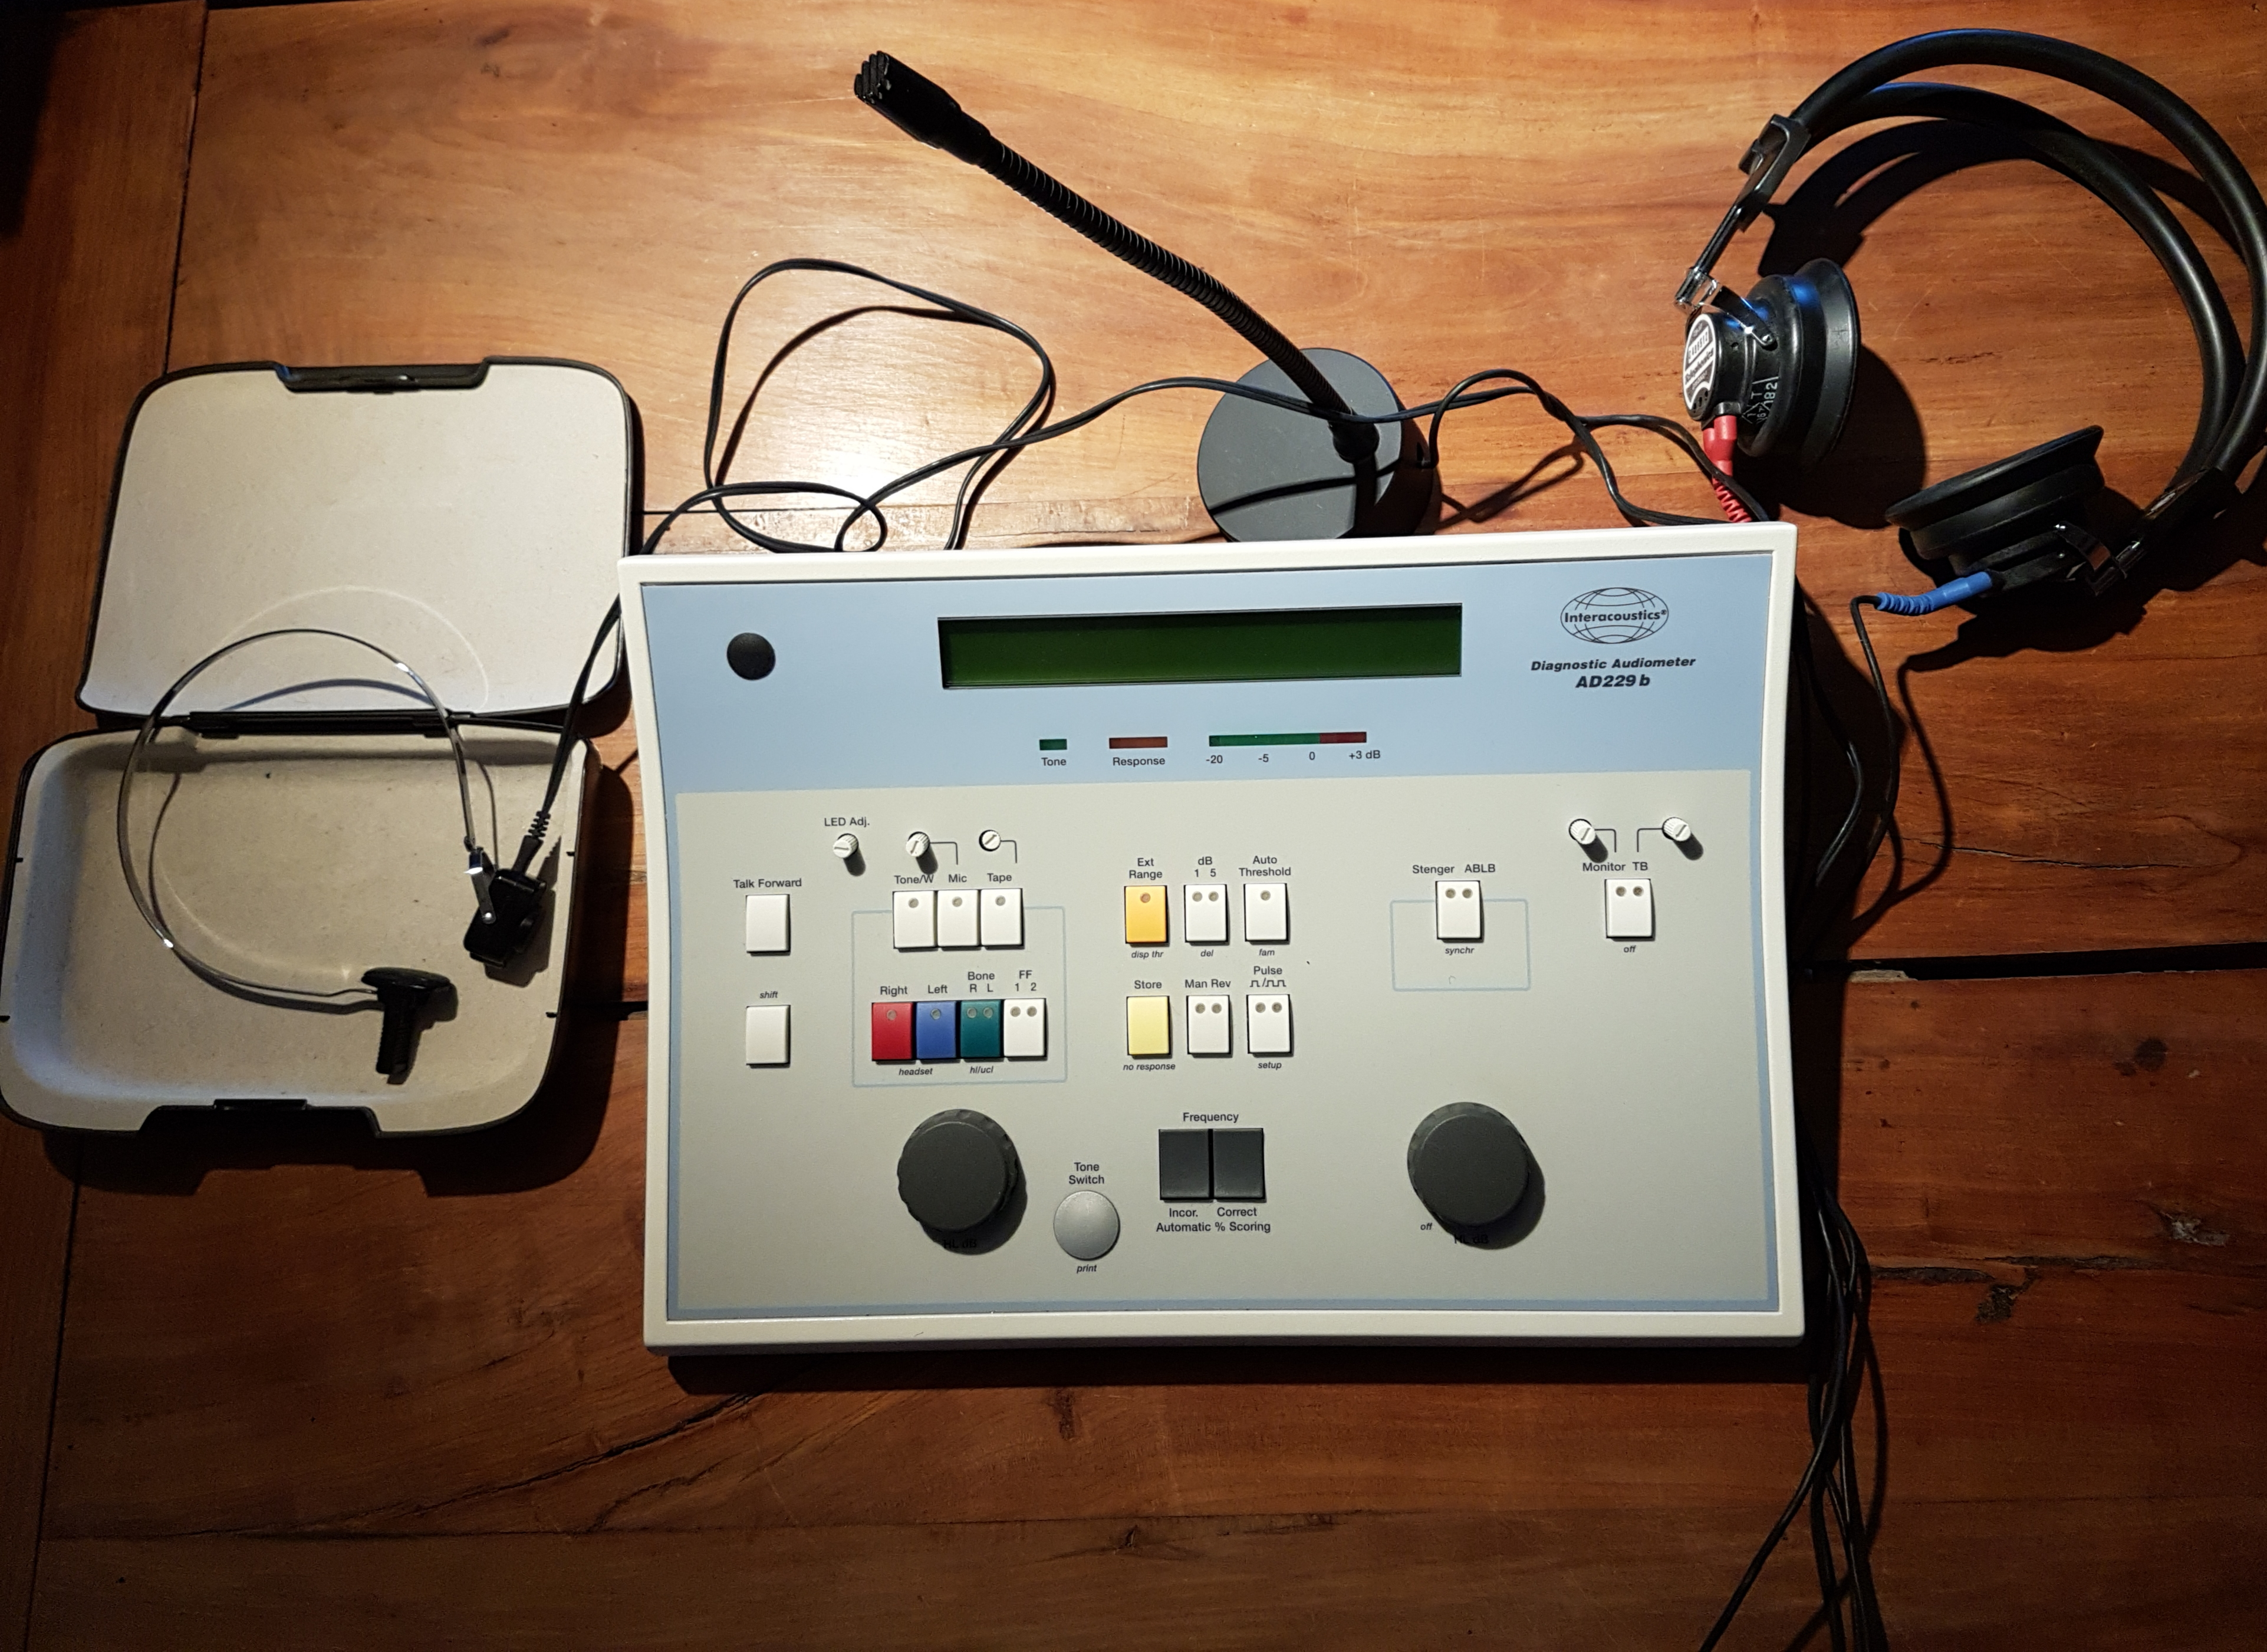
\includegraphics[width=1\linewidth]{images/testecoute.jpg}
	\caption[Appareil test écoute]{Matériel du test d'écoute, écouteurs, vibrateur et micro}
	
	\label{appareiltestecoute}
\end{figure}

\subsection {Le test d'écoute}
Le test d'écoute détecte la manière de recevoir
l'information.
Nous obtenons une
\textbf{représentation graphique} générale des courbes de l'écoute
(équilibre, symétrie, harmonie) à partir des seuils d'écoute
calculés selon les fréquences et le volume que le sujet entend.
%avec des zones à lire et interpréter.
A cet effet, nous utiliserons l'appareil conçu à partir de 1950 par Alfred Tomatis, médecin
O. R. L.: le Hearing Test, testant
l'écoute pré/post - thérapie
afin d'établir une comparaison.
%L'utilisation particulière du \textit{test de perception d'écoute de Tomatis}  est
%légitimée par sa facilité et  simplicité d'application, en dehors de
%son contexte thérapeutique.\footnote{Nous précisons qu'aucun support de la méthode conçue par
%	Tomatis n'interviendra pendant les séances de musicothérapie.}
Nous pourrons constater
s'il existe un changement dans l'écoute du sujet grâce au support graphique, tel un ``dessin'',
une image. %fournissant des critères d'analyse.

\subsection {Le WHO QOL  - Bref}  
Le World Health 	Organisation Quality of Life Assessement  (Cf. Annexe A. 9.) 
est un test d'évaluation de la qualité de vie, issu du
programme de l'Organisation Mondiale de la Santé, l'OMS.
Ce questionnaire est réalisé en parallèle, rempli par
les patients eux-même à l'entrée de leur séjour en clinique et
à leur sortie, avec ou sans musicothérapie.
Il s'agit ici de la version courte  la plus récente (2004) du questionnaire
WHOQOL-100 datant de 1998.
L'utilisation de ce questionnaire a pour but d'avoir
une variable supplémentaire pour confirmer ou infirmer en
parallèle l'action supposée  de la musicothérapie sur une éventuelle
modification de l'écoute.
Il sert aussi à constater s'il y a une\textbf{ transformation psychique }du sujet,
(positive ou négative) et s'il existe ou non une \textbf{corrélation }de
résultats avec le test d'écoute.



\section{Méthode d'analyse}
Nous allons décrire la manière d'analyser et collecter les résultats du questionnaire et du test d'écoute 
avec 15 patients répartis en 2 groupes de même type de pathologie (difficulté de régulation des 
émotions), l'un expérimental avec musicothérapie au nombre de 8 et l'autre, le groupe témoin au nombre 
de 7. 
\subsection{WHOQOL}
L'estimation se fait à partir d'une échelle
d'auto-évaluation subjective avec 26 questions courtes
dont un item concernant la qualité de vie globale
auto-évaluée par le sujet, un item évaluant la santé générale perçue
et les 24 autres se répartissent selon les 4 domaines suivants: physique, psychologique, relations 
sociales et environnement.
\begin{enumerate}
	\item  Le domaine de la perception physique (7 items) comprend l' activité quotidienne// la dépendance 
	et/ou l'assistance médicale// la fatigabilité, l'énergie//la mobilité// la douleur// le sommeil// la capacité 
	de travail//
	\item Le domaine psychologique (6 items):  image de soi, apparence// ressentis positifs et négatifs// 
	estime de soi// spiritualité, croyances personnelles, religion// mémoire et concentration, apprentissage, 
	pensée.
	\item Le domaine des relations sociales (3 items) : relations personnelles// soutien social// vie sexuelle.
	\item Le domaine de l'environnement (8 items) :
	l'environnement domestique et physique
	(pollution, bruit, trafic, climat)// la
	situation financière//  la liberté, la
	sécurité physique et morale//
	l'accessibilité et qualité de la santé// les
	opportunités de détente, loisirs, accès aux
	informations// logement et transport//
\end{enumerate}
Les questions varient selon sa propre perception, telle la satisfaction
au sujet de son  sommeil, de sa vie relationelle, sexuelle, de
l'opinion que l'on a sur soi, \textit{`` Êtes-vous satisfait de
	vous-même?'' , ``Acceptez-vous votre apparence physique?''} par
exemple, ou si le patient éprouve souvent des sentiments négatifs
et s'il a assez d'énergie dans la vie de tous les jours.
Le patient le remplit avec ou sans aide du
thérapeute lors de chaque test
d'écoute.

La cotation se fait sur 4 types d'échelles de réponses en 5 points (de 1 à 5)
permettant l'évaluation de l'intensité, la fréquence, la capacité.
Les résultats et les chiffres obtenus  sont calculés à partir de la moyenne des 4
domaines, pré -- et post -- traitement.
%est calculée pour chaque patient, à partir des scores
%des 4 domaines.
%Les chiffres ont été obtenus à partir des 4
%domaines, avec le pré/post-séjour.

\subsection{Test d'Ecoute: comparatif pré/post-thérapie }

Des graphiques de courbes d'écoute permettent  de synthétiser des différences pré/post traitement des 
deux groupes. %Il s'agit ainsi d'une étude mixant le \textbf{quantitatif  et le
%	qualitatif}.
En procédant toujours en amont et en aval, --- pré/post-thérapie ---, nous
obtenons:
 %par \textbf{comparaison graphique des différentes
%	courbes}: 

%\begin{enumerate}
%	\item   les \textbf{seuils} auditifs --moyenne
%	représentée sous forme de la  \textbf{courbe aérienne}
%	\item   les \textbf{seuils} auditifs --moyenne
%	représentée sous forme de la \textbf{courbe osseuse}
%	\item le nombre de
%	\textbf{croisements}.\footnote{Cf. Ch. 3 A. Tomatis p. 26: les distorsions}
	
%\end{enumerate}


\begin{enumerate}
		\item la \textbf{comparaison des graphiques des différentes courbes}: allure générale, symétrie, 
		équilibre.
	\item la \textbf{moyenne} \textbf{des seuils
		auditifs de la courbe aérienne} de l'oreille \textbf{droite} et de
	l'oreille \textbf{gauche} de \textbf{chaque patient}
	\item la \textbf{moyenne} \textbf{des seuils
		auditifs de la courbe osseuse} de l'oreille \textbf{droite} et de
	l'oreille \textbf{gauche} de \textbf{chaque patient}

	\item le \textbf{nombre de croisements entre courbe aérienne et courbe osseuse}
\end{enumerate}.
%Ainsi, après avoir
%fait une comparaison des dessins des différentes courbes et
%décompté le nombre des croisements, l'ensemble des résultats a été analysé et comparé, puis mis en 
%corrélation avec ceux du\textbf{
%	WHO QOL}.
 \subsection{Les résultats} 
Qu'il s'agisse des tests ou des questionnaires, nous avons choisi de
simplifier les résultats sous forme de signes
mathématiques,  \textbf{ $+$, $=$, $-$ } avec les significations suivantes.


\textbf { Les test d'écoute: } 


Avec  le graphique des courbes:
\begin{enumerate}
	\item$+$   : amélioration, modification;  rapprochement significatif à la courbe dite idéale.
	\item$=$   : amélioration insignifiante, correspond à : $+/-$, (si c.a. $ + $ et c.o. $-$, ou vice-versa).
	
	\item$-$   : pas d'amélioration et pas/trop peu  de modification, inversion
	des courbes (c.o. supérieure à c.a.).
	
	Avec les \textbf{croisements}, les chiffres des tests pré/post
	nous permettent d'obtenir une comparaison:
	\item $+$ : plus petit est le nombre, meilleur est le résultat, ce qui correspond à un signe positif : $+$.
	\item$-$   : plus grand est le nombre, ce sera un signe négatif: $-$.
\end{enumerate}

\textbf{Le questionnaire WHO QOL:} 	
\begin{enumerate}
\item$+$  :  le score chiffré  en fin de séjour est plus élevé
que celui du
pré-séjour, le résultat final obtenu est considéré comme
positif et sera relevé  avec le signe : "+". 
\item $-$ : le score est plus bas, il  sera considéré comme négatif : "-"  
\item$=$ : le score pareil, sans changement,  comme avant le séjour, il sera reconnu sous le signe :  "=" .

Ensuite, pour créer le lien et la corrélation entre test écoute et questionnaire WHO QOL, nous ferons la 
somme finale des résultats des signes.
\end{enumerate}
\section{Design de l'étude}

\textbf{L'étude} est
réalisée en fonction des séjours variables des patients, soit une
totalité  de quatre semaines
distribuées dans l'intervalle juin --
octobre 2017,  à l'aide de tests et questionnaires appliqués en début
et fin de séjour.

La figure suivante décrit de manière succinte le déroulement de
l'étude sur la durée avec les deux groupes.



\begin{figure}[hb]
	\centering
	\includegraphics[width=1\linewidth]{images/Groupecontrole.png}
	\caption[Schéma du déroulement]{Déroulement de l'étude avec GM et GC}
	
	%\label{groupecontroleimage1}
\end{figure}


\textbf{Procédure}
Chaque participant du groupe GM et GC va faire en entrée et en sortie de
clinique, après environ 4 semaines, un
test avec questionnaire  WHO QOL. (GM ayant suivi une musicothérapie active et/ou réceptive (1x par
semaine).
Chaque test d'écoute dure
70 à 90 minutes, fait 2x (pré/post-thérapie) et
suivi du questionnaire WHOQOL (2x10') rempli par le
patient lui-même.

Sur \textbf{44 tests d'écoute} réalisés pour \textbf{GC et GM},
nous avons décompté\textbf{ 30 tests} valides qui serviront de
comparatif dont \textbf{16} pour
GM, groupe de musicothérapie et \textbf{14 tests d'écoute} pour GC, le groupe
contrôle.

\begin{figure}
	\centering
	\includegraphics[width=1\linewidth]{images/graphiques/Testecoute.png}
	\caption{Nombre de tests d'écoute avec GM et GC}
	
	%\label{groupecontroleimage1}
\end{figure}



\begin{figure}
	\centering
	\includegraphics[width=1\linewidth]{images/graphiques/TestWQ.png}
	\caption{Nombre de WHO QOL avec GM et GC}
\end{figure}





%\textbf{Index courbe idéale aérienne et osseuse}:
%La moyenne chiffrée de la courbe aérienne: 1,3
%La moyenne chiffrée de la courbe osseuse: 3,11
%Remarque: nous n'avons pas pu ici montrer l'intégralité des tests d'écoute, mais ceux-ci se trouvent à 
%disposition sur demande et en toute confidentialité.
%Notons que nous avons évidemment fait l'ensemble de l'analyse.
%Nous présenton
%Nous allons entrer dans l'étude clinique.
 Pour chaque patient : 2 tests d'écoute et 2 
questionnaires WQ 
remplis.
Le grand problème rencontré a été de pouvoir obtenir un nombre suffisant  de WQ remplis en fin de 
séjour dans le groupe de musicothérapie.
% Cela nous a 
%conduit à 
%la difficulté d'obtenir un nombre égal pour comparer.
Le nombre de tests d'écoute a été obtenu en parallèle pour les 2 groupes mais pas pour le questionnaire.
Ce qui a eu comme incidence de réduire considérablement la démonstration de cas proposés.
Voilà la manière dont s'est déroulée cette étude.
%pour aller jusqu'au bout de ce que nous avions décidé au départ, 
Nous nous sommes donc tenus à notre plan, constatant des données  manquantes mais 
indépendamment de notre volonté.
% et avons donc hésité à le signaler mais nà ne plus prendre en 
%compte cette parallèle. L'étude aurait été tronquée.
% aà chaque fois après 

%\part{La pratique}
\chapter[\'Etude clinique]{\'Etude clinique}

%Souvenons-nous brièvement de l'évolution de la signification du terme
%``clinique'' enraciné dès l'Antiquité.
%A l’origine,\textbf{ l’activité clinique} (<gr. klinê = le lit) est celle du médecin qui, au chevet du malade, procède à l’examen des manifestations de la maladie (méthode de l’observation, de l’interrogation et de l’écoute) en vue de poser un diagnostic*, un pronostic* et une prescription* de traitement.
%Michel Foucault (1926-†1984), psychologue français, dans son ouvrage capital de 1963,
%«Naissance de la clinique» nous rend attentifs au fait que l’adjectif «clinique» fut longtemps du monopole médical, avec %l’observation « naturelle » faite au lit du malade, uniquement à l’aide des organes sensoriels.

%Hippocrate (médecin grec, Cos 460-377) était clinicien : il apprenait à ses étudiants l’art d’observer les symptômes, ceux-ci étant les réactions d’une personnalité à une agression pathogène. Généralisation et rationalisation, selon les critères d’Aristote, permettaient l’élaboration de « ces entités nosologiques* », les maladies, qui s’emparaient du corps du malade et poussant les médecins, exorcistes laïques, à les en faire sortir.
%Les publications de Th.Ribot à la Sorbonne rejoignent [avec «La psychologie des sentiments »(1896), «Les maladies de la mémoire »(1883) et «Les maladies de la personnalité » (1885)], les idées de S. Freud, montrant la primauté de la vie affective, où les tendances inconscientes jouent un rôle fondamental, et pouvant s’extérioriser soit par l’arrêt du développement affectif, soit par la dissolution des acquisitions plus récentes.

%L’expression « psychologie clinique » apparaît sous la plume de S. Freud, dans sa lettre à W. Fliess du 30.01.1899 : « Maintenant, la connexion avec la psychologie, telle qu’elle se présente sur les Etudes sur l’hystérie(1895) sort du chaos, j’aperçois les relations avec le conflit, la vie, tout ce que j’aimerais appeler psychologie clinique ». 

%La définition « officielle » de la psychologie clinique mobilise et articule la singularité et
%la totalité, de façon à reconnaître une discipline psychologique basée sur l’étude approfondie des cas individuels, l’étude de la conduite humaine individuelle et de ses conditions (hérédité, maturation, conditions psychologiques et pathologiques, histoire de la vie), en somme, l’étude de la personne totale «en situation», c.à.d. l’expérience vécue de ce rapport à l’environnement.

%Au vue de cet aperçu historique, on peut reconnaître que
%dans certains milieux psychiatriques actuels, la musicothérapie trouve plus sa place aussi dans le complètement des tableaux cliniques.

Dans notre étude, l'axe principal porte sur la
vérification de l'amélioration de
la capacité d'écoute suite au travail musicothérapeutique.
Nous allons
d'abord exposer le cadre dans lequel nous avons fait ces tests, la
population étudiée et procéder à la comparaison des modifications de
l'écoute.

\section{Méthode}

 La clinique privée (Privatklinik)
de Meiringen (BE) est  principalement spécialisée en
addictologie avec problèmes d'alcool et de toxicodépendance, couvrant aussi les aspects dépressifs
et les
burnouts.


Elle dispose d'une capacité de 195 lits, et le temps de séjour fluctue de 3 à 6 semaines ou plus, en
fonction de la participation des assurances.

Actuellement, en plus de l'administration et l'intendance, les 33
médecins et psychiatres, sont
accompagnés par 177
soignants, dont infirmiers psychiatriques, aide-infirmières, physio et
ergothérapeutes, 
psychologues et intervenants en \textit{thérapies
créatives}, comme l'art-thérapie, thérapie
corporelle, zoothérapie (chien/cheval),  ateliers de créativité --
bois et terre --,  les textiles et la\textbf{ musicothérapie} avec deux
personnes, dont la souscrite à titre de 10 pour cent.


%\textbf{Organigramme}: nous avons obtenu l'autorisation de vous
%montrer l'organigramme de la Clinique de Meiringen lors de la
%soutenance.




%(-OH*:  le radical hydroxile, oxydrile de la molécule éthylique)


\subsection{Population}
L'\textbf{échantillonnage} fortement conditionné par les contraintes
institutionnelles, comme les interruptions prématurées de séjour, les rendez-vous
 médicaux superposés, l'impossibilité de participation physique et/ou
 psychique, les remplacements disparates et hétéroclites de ma
 collègue, l'emploi à
 temps partiel, a été restreint  par le choix d'un nombre limité de
 patients (N=29).
Une autre contrainte de nature extra-institutionnelle allant dans le
même sens réside dans l'éloignement géographique.

\textbf{Le Groupe Musicothérapeutique (expérimental) GM} comporte 21
patients, dont 6
femmes et 15 hommes.

\textbf{Le  Groupe Contrôle GC} comporte 8 patients, dont 4 femmes et 4 hommes.

Le nombre
des patients s'est limité  à 8
patients (4 hommes/4 femmes) pour le GM, et à 7 patients (4 hommes/3
femmes) pour le GC pour obtenir une comparaison entre les tests et les questionnaires.




En synthèse:
 \begin{itemize}
 
 \item \textbf{Nombre total de personnes}: N= 29 
\item\textbf{Genre et âge de la population étudiée:}  19 hommes et 10 femmes, de 25 à 72
  ans dont l'âge moyen est de 48 ans.
 \item\textbf{Pathologies}: troubles de la régulation émotionnelle
   dont le burnout, les dépendances, la dépression.
   Il n'a pas été
   possible de différencier les pathologies, car la pose de
   diagnostic dans ce domaine reste toujours difficile et délicat pour le corps médical, raisons pour lesquelles elles
   se trouvent traitées ensemble.
 \item \textbf{Total de séances} par personne en
   musicothérapie= 4 ;   \textbf{mu}=1/semaine;  
 \textbf{t}= 50--60 min, période = 3 -- 4 semaines.
\end{itemize}




 %mu en grec
\subsection{Démarches}
Obtenu l'aval de la direction de la
clinique pour cette étude,  le personnel soignant et l'ensemble des
thérapeutes (ateliers, thérapies créatives, kynési--cyno--
et hippothérapie) vont être informés aussi par écrit.

Ce même texte, destiné aux
patients\footnote{Cf.Annexe A.7} explique le projet de l'étude sur l'écoute, comme aussi la transformation
avec ou sans musicothérapie.
Le consentement libre est validé par la signature du patient, après
un court entretien avec lecture.\footnote{Cf. Annexe A.10}.
%\footnote{Regula
  %Lehmann, musicothérapeute  à 90\%  à la clinique de Meiringen.} 


Après ces prémisses, l'étude commence véritablement avec l'application du test
audiométrique suivie du questionnaire qualitatif.

\textbf{L'étude} est
réalisée en fonction des séjours variables des patients, soit une
totalité  de quatre semaines
distribuées dans l'intervalle juin --
octobre 2017,  à l'aide de tests et questionnaires appliqués en début
et fin de séjour.

\textbf{Types de thérapie, musicothérapie} réceptive et/ou active.
Les autres formes de thérapies, en gardant
leur indépendance par rapport à notre analyse, se déroulent simultanément, à
l'exception de la musicothérapie pour le groupe contrôle.


\subsection{Matériel (tests et questionnaires)}
	Nous utiliserons deux tests différents : 
	le test d'écoute spécifique d'Alfred Tomatis
	et le test-questionnaire, le WHO QOL-Bref, les deux qualitatifs et quantitatifs.

        
        \textbf{Le test d'écoute}
        \footnote{Cf. Ch. 3. A. Tomatis p.27} détecte la manière de recevoir
        l'information. 
Nous obtenons une  
	\textbf{représentation graphique} générale des courbes de l'écoute
        (équilibre, déséquilibre, harmonie) à partir des seuils d'écoute
        calculés selon les fréquences et le volume que le sujet entend
        avec des zones à lire et interpréter.
	A cet effet, nous utiliserons l'appareil conçu à partir de 1950 par Alfred Tomatis, médecin
        O. R. L.: le Hearing Test, ou TLST, testant
        l'écoute pré/post-thérapie
        afin d'établir une comparaison.
        L'utilisation particulière du \textit{test de perception d'écoute de Tomatis}  est
légitimée par sa facilité et  simplicité d'application, en dehors de
son contexte thérapeutique.\footnote{Nous précisons qu'aucun support de la méthode conçue par
        Tomatis n'interviendra pendant les séances de musicothérapie.}
      Nous pourrons constater
      s'il existe un changement dans l'écoute du sujet grâce au support graphique, tel un ``dessin'',
      une image. %fournissant des critères d'analyse.
      
        Le\textbf{ WHO QOL  - Bref:  World Health
   Organisation Quality of Life Assessement } (Cf. Annexe A.9.) est un test d'évaluation de la qualité de vie, issu du
	programme de l'Organisation Mondiale de la Santé, l'OMS.
	Ce questionnaire est réalisé en parallèle, rempli par
        les patients eux-même à l'entrée de leur séjour en clinique et
        à leur sortie, avec ou sans musicothérapie.
 L'utilisation de ce questionnaire a pour but d'avoir
 une variable supplémentaire pour confirmer ou infirmer en
parallèle l'action supposée  de la musicothérapie sur une éventuelle
modification de l'écoute.

Il sert aussi à constater s'il y a une\textbf{ transformation psychique }du sujet,
 (positive ou négative) et s'il existe une \textbf{corrélation }de
 résultats avec le test d'écoute.

 
        L'estimation se fait à partir d'une échelle
d'auto-évaluation subjective avec 26 questions courtes 
--il s'agit ici de la version courte  la plus récente (2004) du questionnaire
 WHOQOL-100 datant de 1998, --
dont un item concernant la qualité de vie globale
auto-évaluée par le sujet, un item évaluant la santé générale perçue
et les 24 autres se répartissent selon les 4 domaines suivants: physique, psychologique, relations sociales et environnement.
\begin{enumerate}
\item  Le domaine de la perception physique (7 items) comprend l' activité quotidienne// la dépendance et/ou l'assistance médicale// la fatigabilité, l'énergie//la mobilité// la douleur// le sommeil// la capacité de travail//
	\item Le domaine psychologique (6 items):  image de soi, apparence// ressentis positifs et négatifs// estime de soi// spiritualité, croyances personnelles, religion// mémoire et concentration, apprentissage, pensée.
		\item Le domaine des relations sociales (3 items) : relations personnelles// soutien social// vie sexuelle.
			\item Le domaine de l'environnement (8 items) :
                         l'environnement domestique et physique
                         (pollution, bruit, trafic, climat)// la
                         situation financière//  la liberté, la
                         sécurité physique et morale//
                         l'accessibilité et qualité de la santé// les
                         opportunités de détente, loisirs, accès aux
                         informations// logement et transport// 
\end{enumerate}
		Les questions varient selon sa propre perception, telle la satisfaction
au sujet de son  sommeil, de sa vie relationelle, sexuelle, de
l'opinion que l'on a sur soi, \textit{`` Êtes-vous satisfait de
vous-même?'' , ``Acceptez-vous votre apparence physique?''} par
exemple, ou si le patient éprouve souvent des sentiments négatifs
et s'il a assez d'énergie dans la vie de tous les jours.
La cotation se fait sur 4 types d'échelles de réponses en 5 points (de 1 à 5)
permettant l'évaluation de l'intensité, la fréquence, la capacité, l'évaluation.
Le patient le remplit avec ou sans aide du
thérapeute lors de chaque test
d'écoute.

La figure suivante décrit de manière succinte le déroulement de
l'étude sur la durée avec les deux groupes.



        \begin{figure}[hb]
\centering
\includegraphics[width=0.7\linewidth]{images/Groupecontrole.png}
\caption[Schéma du déroulement]{Déroulement de l'étude avec GM et GC}
       
%\label{groupecontroleimage1}
\end{figure}
	
 \subsection{Procédure}
Chaque participant du groupe GM et GC va faire en entrée et en sortie de
clinique, après environ 4 semaines, un
          test avec questionnaire  WHOQOL. (GC ayant suivi une musicothérapie active et/ou réceptive (1x par
        semaine).\footnote{Voir Fig. 4.1.}
          Chaque test d'écoute dure
        70 à 90 minutes, fait 2x (pré/post-thérapie) et 
        suivi du questionnaire WHOQOL (2x10') rempli par le
        patient lui-même.
        
Sur \textbf{44 tests d'écoute} réalisés pour \textbf{GC et GM},
      nous avons décompté\textbf{ 30 tests} valides qui serviront de
     comparatif dont \textbf{16} pour
     GM, groupe de musicothérapie et \textbf{14 tests d'écoute} pour GC, le groupe
     contrôle.
      \begin{figure}
\centering
\includegraphics[width=1\linewidth]{images/graphiques/test_ecoute.jpg}
\caption[Schéma du déroulement]{Nombre de tests d'écoute avec GM et GC}
       
%\label{groupecontroleimage1}
\end{figure}

Sur \textbf{25 questionnaires WHOQOL}, il y a \textbf{10 pour GM} remplis
avec 8 pré- et seulement 2
     post- thérapies; et \textbf{15 pour GC} dont 8 pré-
     et 7 post-thérapie.
      Nous avons dans l'ensemble un total de \textbf{9 questionnaires} pour le
     comparatif des 2 groupes réunis.
    
\textbf{ Pathologie des groupes}: Les patients ont été répartis en deux groupes sans différenciation de
 leur pathologie. Nous avons conscience d'avoir mélangé des symptomatologies qui
 toutefois paraissent
 sous-tendues par
                                               certains mécanismes
                                               similaires dont le
                                               noyau commun est une
                                              \textbf{difficulté de
                                               régulation des
                                               émotions}, 
                                               s'exprimant par une
                                               humeur négative.
                                               Il convient ici de mentionner que, en vue de la taille réduite des échantillons, il n'est pas
pertinent de se lancer dans une analyse purement
quantitative.

\section{Hypothèses opérationnelles}

Il s'agit ainsi d'une étude mixant le \textbf{quantitatif  et le
  qualitatif}.
En procédant toujours en amont et en aval, --pré/postpostthérapie--, nous
avons obtenu la \textbf{moyenne} \textbf{des seuils
auditifs de la c.a. et de la c.o.} de l'oreille \textbf{droite} et de
l'oreille \textbf{gauche} de chaque patient, ci-dessous illustrée par
plusieurs exemples. Ensuite, après avoir 
fait une comparaison des dessins des différentes courbes et
décompté le nombre des croisements, l'ensemble des résultats sera analysé et comparé.
Nous ferons ensuite la corrélation des résultats avec ceux du\textbf{
  WHOQOL}.

Qu'il s'agisse des tests ou des questionnaires, nous avons choisi de
simplifier les \textbf{résultats} sous forme de signes
mathématiques, $+$, $=$, $-$ avec les significations suivantes.
Avec les \textbf{tests d'écoute}: 
\begin{enumerate}
\item$+$   : amélioration, modification;  rapprochement significatif à la courbe dite idéale.
\item$=$   : amélioration insignifiante, correspond à : $+/-$, (si c.a. $ + $ et c.o. $-$, ou vice-versa).

\item$-$   : pas d'amélioration et pas/trop peu  de modification, inversion
des courbes (c.o. supérieure à c.a.). 

  Avec les \textbf{croisements}, les chiffres des 2 tests pré/post
  nous permettent d'obtenir une comparaison: 
  \item Plus petit est le nombre, meilleur est le résultat, ce qui correspond à un signe positif : $+$.
\item Dans le
  cas contraire, ce sera un signe négatif: $-$.
  
\end{enumerate}


 \subsection{ Comparaison pré/post-thérapie des résultats du test d'écoute}
Avec les tests d'écoute, nous 
allons donc prendre en compte:

\begin{enumerate}
 \item   les \textbf{seuils} auditifs --moyenne
représentée sous forme des \textbf{courbes aérienne et osseuse} --
\item  l'observation par \textbf{comparaison graphique des différentes
  courbes}
\item le nombre de
\textbf{croisements}.\footnote{Cf. Ch. 3 A. Tomatis p. 26: les distorsions}
 
\end{enumerate}


%\textbf{Index courbe idéale aérienne et osseuse}:
%La moyenne chiffrée de la courbe aérienne: 1,3
%La moyenne chiffrée de la courbe osseuse: 3,11


  Nous allons commencer par l'observation de trois patients du Groupe Contrôle.
     

      \textbf{Groupe Contrôle : Observation avec 3 patients}
  \paragraph{ A. Patient Br.:}
  \begin{figure}[ht]
\centering
\includegraphics[width=0.7\linewidth]{images/graphiques/bru_pre.png}
\caption[Moyenne OG+OD]{Premier test Br.}
       
%\label{groupecontroleimage1}
\end{figure}



 \begin{figure}[th]
\centering
\includegraphics[width=0.7\linewidth]{images/graphiques/bru_post.png}
\caption[Moyenne OG+OD]{Second test Br.}
       
%\label{groupecontroleimage1}
\end{figure}

	\begin{enumerate}
 		\item  c.a.: pas de modification, augmentation des
                  seuils: $-$
 		\item  c.o.: redressement des seuils: $+$
 		\item  croisements: $5/4$ : $+$ : ce qui signifie:  5 croisements lors du 1°test// 4 croisements lors du 2° test= nous avons 1 croisement en moins, donc le résultat est considéré comme positif en fin
                  de séjour.
                \end{enumerate}

                \textbf{  Conclusion:  -    +    +       :  +}




\paragraph{B. Patient Sch.:}

	\begin{enumerate}
 		
 		\item : c.a.: pas de modification, très légère augmentation des
                  seuils: +/-
 		\item : c.o.: a passé sous c.a., modification des seuils: +
 		\item : croisements: 2/2 :     =
                   \end{enumerate}
 \textbf{  Conclusion:  +/-    +    =        :  =}

\begin{figure}
\centering
\includegraphics[width=0.7\linewidth]{images/graphiques/schaff_pre.png}
\caption[Moyenne OG+OD]{Premier test Sch.}
       
%\label{groupecontroleimage1}
\end{figure}


         \begin{figure}
\centering
\includegraphics[width=0.7\linewidth]{images/graphiques/schaff_post.png}
\caption[Moyenne OG+OD]{Second test Sch.}
       
\label{groupecontroleimage1}
\end{figure}


\paragraph{C. Patient Wal.:}



\begin{figure}
\centering
\includegraphics[width=0.7\linewidth]{images/graphiques/wal_pre.png}
\caption[Moyenne OG+OD]{Premier test Wal.}
       
%\label{groupecontroleimage1}
\end{figure}

	\begin{enumerate}
 		
 		\item : c.a.: peu de modification: =
                
 		\item : c.o.: reste dominante, tentative de rapprochement de c.a.: -
 		\item : croisements: 1/3 :  -
                  
                \end{enumerate}

                \textbf{ Conclusion:  $= -  -        : -$ }

               \begin{figure}
\centering
\includegraphics[width=0.7\linewidth]{images/graphiques/wal_post.png}
\caption[Moyenne OG+OD]{Second test Wal.}
       
\label{groupecontroleimage1}
\end{figure}
                
  \textbf{ Groupe de Musicothérapie: Observation avec 4 patients}

\paragraph{ A. Patient Sw.:}



 \begin{figure}[th]
\centering
\includegraphics[width=0.7\linewidth]{images/graphiques/sw_pre.png}
\caption[Moyenne OG+OD]{Premier test Sw.}
       
%\label{groupecontroleimage1}
\end{figure}

	\begin{enumerate}
 		
 		\item : c.a.: pas de modification: = %  1,27/1,27
                
 		\item : c.o.: redressement et rapprochement,
                  relèvement des seuils: -       %  3,07/3,39
 		\item : croisements: 1/3 :  -
                  
                \end{enumerate}

                \textbf{  Conclusion:  = +  -        : ``=''}

                \begin{figure}
\centering
\includegraphics[width=0.7\linewidth]{images/graphiques/sw_post.png}
\caption[Moyenne OG+OD]{Second test Sw.}
       
%\label{groupecontroleimage1}
\end{figure}




\paragraph{B. Patient Cav.: }

(pas de WOQOL fin de séjour)


\begin{figure}[th]
\centering
\includegraphics[width=0.7\linewidth]{images/graphiques/cav_pre.png}
\caption[Moyenne OG+OD]{Premier test Cav.}
       
%\label{groupecontroleimage1}
\end{figure}

	\begin{enumerate}
 		
 		\item : c.a.: redressement: +
                
 		\item : c.o.: redressement et rapprochement, relèvement des seuils: +
 		\item : croisements: 3/1 :  +
                  
                \end{enumerate}

                \textbf{  Conclusion:  + + +       : ``+''}

                \begin{figure}
\centering
\includegraphics[width=0.7\linewidth]{images/graphiques/cav_post.png}
\caption[Moyenne OG+OD]{Second test Cav.}
       
%\label{groupecontroleimage1}
                \end{figure}



                
               \paragraph{ C. Patient M.:}


	\begin{enumerate}
 		
 		\item : c.a.: redressement: : +   % 6,43/6,03
                
 		\item : c.o.: redressement et rapprochement,
                  relèvement des seuils:  +     %6,25/5,85:
 		\item : croisements: 3/3 :  =
                  
                \end{enumerate}

                \textbf{  Conclusion:  +  +  =     : ``+''}

                \begin{figure}
\centering
\includegraphics[width=0.7\linewidth]{images/graphiques/m_pre.png}
\caption[Moyenne OG+OD]{Premier test M.}
       
%\label{groupecontroleimage1}
\end{figure}


                        \begin{figure}
\centering
\includegraphics[width=0.7\linewidth]{images/graphiques/m_post.png}
\caption[Moyenne OG+OD]{Second test M.}
       
%\label{groupecontroleimage1}
\end{figure}


                
\paragraph{D. Patient K.:}

  (pas de WOQOL fin de séjour)

        \begin{figure}
\centering
\includegraphics[width=0.7\linewidth]{images/graphiques/kad_pre.png}
\caption[Moyenne OG+OD]{Premier test K.}
       
%\label{groupecontroleimage1}
\end{figure}
	\begin{enumerate}
 		
 		\item : c.a.: redressement important: +
                
 		\item : c.o.: rapprochement et relèvement des seuils: +
 		\item : croisements: 1/7 :  -
                  
                \end{enumerate}

                \textbf{  Conclusion:  + + -       : ``+''}

                 \begin{figure}
\centering
\includegraphics[width=0.7\linewidth]{images/graphiques/kad_post.png}
\caption[Moyenne OG+OD]{Second test K.}
       
%\label{groupecontroleimage1}
\end{figure}
          
\paragraph{ Conclusions et résultats:}

             Nous nous trouvons
           en présence de deux groupes, un groupe de contrôle et un
           groupe de musicothérapie ayant le même type de
           pathologie --difficulté de régulation des émotions-- avec la constatation suivante: il existe 
          une \textbf{modification de l'écoute pré- et post-traitement}.
          Cette modification est nettement plus marquée
          pour GM, groupe de musicothérapie, le résultat est positif, que pour le groupe de contrôle, GC.

          \textbf{GM: ``+''}.

          
          \textbf{GC:  ``='' ou +/-}.

          
        Les données quantitatives observables dans ces graphiques semblent aller dans le
sens de  l'étude faite par le
CNRS (Cf. Ch. Introduction, p. 16) \autocite{affectiveDisorders} réalisée à partir des seuils auditifs, à savoir
les patients souffrant de troubles post-traumatiques souffrent d'un
appauvrissement caractéristique de fréquences.


\subsection{ Comparaison pré/post-thérapie des résultats des
  questionnaires WHOQOL}

\begin{figure}[tbh]
\centering
\includegraphics[width=1.2\linewidth]{images/graphiques/questionnaire_wq.png}
\caption[Questionnaire WHOQOL-BREF]{GM/GC - Pré/Post avec la moyenne des scores par domaine}
       
%\label{groupecontroleimage1}
\end{figure}
Voici à présent ci-dessus le schéma (fig.5.17) représentant la
moyenne pré- et post-traitement, calculée pour chaque patient, des scores
des 4 domaines.
%Les chiffres ont été obtenus à partir des 4
%domaines, avec le pré/post-séjour.
Remarque: si, par comparaison, le chiffre post-séjour est plus élevé
que celui du
pré-séjour, le résultat final obtenu est considéré comme
positif. Par conséquent, nous
observerons soit un score négatif, positif ou égal (sans changement).


Nous avons mis en détail  à titre d'exemple 3 patients du GC et 2 du GM
afin d'être le plus clair possible
dans notre façon de procéder.
A la fin, nous avons illustré en couleur (Fig. 5.18 et 5.19.) les
résultats finaux des deux groupes au complet avec 2 schémas
comparatifs.

\paragraph{ GC: Représentation des résultats avec 3 patients du groupe contrôle:}

\begin{enumerate}
\item : A. Patient Br.:  25/27 - 21/22 - 12/11 - 33/32 =  ''-''
  
          Résultat: 21,6 contre 23 pré-traitement,  ce qui
        correspond au signe négatif.
      \item : B. Patient Sch.: 30/27 - 20/20 -  10/10 - 35/30 = ''-''
        
         Résultat: 21,75 contre 23,75 pré-traitement, ce qui
        correspond au signe négatif.
              
 		\item :  C. Patient Wal. : 24/19 -  17/18 - 6/5 -
                  27/20 =  ''-''

                  Résultat: 15,5 contre 18,5 pré-traitement, ce qui
        correspond au signe négatif.
 	\end{enumerate}
        

       \textbf{ Conclusion}: les résultats sont \textbf{négatifs}.
        Ces exemples confirment  
        le ressenti subjectif moyen de l'ensemble des patients
        GC post-traitement, comme représenté à la Figure 5.18.

       \textbf{ GM: Représentation de résultats avec 2 patients du groupe de musicothérapie}

\begin{enumerate}
 		\item : A. Patient Sw. : 26/25 - 19/19 - 8/8 - 29/30 =  ''='' 
                
                
                
  Résultat: 20,5 contre 20,5 pré-traitement, ce qui
        correspond au signe égal.



 		\item : B. Patient M.: 17/27 - 13/23 -  9/10 - 24/32 = ``++''
 	
              Résultat: 23 contre 15,75 pré-traitement, correspondant
              au signe positif. 
            \end{enumerate}
            
                 Ainsi,  GM s'exprime
                 \textbf{positivement }
                 sur l'ensemble du séjour en clinique.

    
                
\begin{figure}
\centering
\includegraphics[width=0.7\linewidth]{images/Compcontrole.png}
\caption[Schéma du déroulement]{WHOQOL:  GC. Comparatif avant/après séjour}
       
%\label{groupecontroleimage1}
\end{figure}

\begin{figure}
\centering
\includegraphics[width=0.7\linewidth]{images/Compmusico.png}
\caption[Schéma du déroulement]{ WHOQOL: GM. Comparatif pré/post-traitement }
       
%\label{groupecontroleimage1}
\end{figure}


Nous avons obtenu un comparatif graphique  des résultats des
                 questionnaires pré/post-traitement du groupe de contrôle,
                 puis du groupe de musicothérapie, graphiques se trouvant sous les fig.5.18 et 5.19.
       En résumé, nous observons que, selon les chiffres obtenus, le ressenti
       subjectif d'amélioration psychique 
        des patients suivis en musicothérapie apparait comme
        supérieur.
        De manière générale, l'ensemble des données des deux groupes représentés
        par les graphiques corrobore ce résultat.
        Ces données sont des valeurs indicatives car nous avons conscience que l'échantillonnage ne
        peut pas être représentatif, comme déjà dit plus haut, dû
        notamment à un
        manque de
        questionnaires WQ, raisons pour lesquelles nous avons
        restreint le nombre d'exemples WQ présentés ici, pour obtenir
        une parité avec les tests d'écoute et obtenir la
        \textbf{corrélation test d'écoute et questionnaire} qui va
        suivre immédiatement.
        
  \subsection{Corrélation des résultats des tests d'écoute et des
    résultats des WQ avec Groupe Contrôle et
    Groupe Musicothérapie:}
\textbf{Groupe Contrôle:} 	          \textbf{ test d'écoute: ``=''   et    WQ: ``-'}

 
\textbf{Groupe Musicothérapie:}     \textbf{test d'écoute: ``+''      et    WQ: ``+''}


 \begin{figure}[th]
\centering
\includegraphics[width=1\linewidth]{images/graphiques/comparaison_pre_post.png}
\caption[Corrélation résultats pré/post]{Comparatif
  pré/post-traitement, WHOQOL, test d'écoute, GM, GC.}
       
\label{comparaison_pre_post}
\end{figure}



                Nous relevons l'impact positif de la
                musicothérapie sur GM.
                De plus, le résultat est renforcé par la corrélation
                avec le WQ.

                
                Pour GC, l'ensemble des résultats sont neutres pour le
                test d'écoute. En ce qui concerne le
                regard des patients sur eux-même avec le WQ, il est
                même négatif. Avec les patients du Groupe de
              Contrôle, nous remarquons grâce aux tests une courbe aérienne
              sans modification mais une courbe osseuse plus
              particulièrement réactive. Contrairement à
              ce que le patient pouvait ressentir ou estimer, il y a indication  et attestation d'une amorce de
              processus intérieur et ce, par un autre biais, celui de
              la transformation de son 
              écoute.
              
 Par ailleurs, indistinctement pour les deux
 groupes,il existe ainsi pour le thérapeute des
 suggestions de différentes pistes de travail dans le but de 
 solliciter le patient plus spécifiquement en se référant aux
              différentes zones (Cf.chéma 6.19), également zones
 d'élaboration psychique. Ce peut être, par exemple,
              l'expression verbale, si la courbe aérienne est restée
              totalement ``muette'' et la zone 2 non
              réactive.

              Pour le groupe de contrôle, visiblement, le travail
                thérapeutique pouvait être plus accentué dans ce
                sens, renforcé à plus forte raison sous la forme musicothérapeutique, pour soutenir le
                patient dans sa transformation et mise en résonance
                interpersonnelle.

                
                Par conséquent,  le test d'écoute a
                apporté un autre regard avec des compléments d'informations au questionnaire
                WQ.

                En\textbf{ conclusion}, le test
                d'écoute est une source de données similaires
                et/ou complémentaires et peut, par conséquent, être
                considéré comme \textbf{révélateur d'un
                travail en musicothérapie}.

 \section{Les séances de musicothérapie}
               Lors de leur déroulement, les séances de
               musicothérapie n'ont pas été 
décortiquées pour analyser leur impact. C'eût
été passionnant de le faire mais ce n'était pas notre objectif.


Par contre, nous avons fait quelques rapprochements intéressants dans les perspectives d'une analyse plus
poussée et plus importante pour laquelle nous avons  relié\textbf{ les trois zones du
test d'écoute avec des données musicothérapeutiques.}
(Fig.6.19).
Nous avons aussi mis 
en parallèle  l'utilisation d'instruments,(Cf. Annexe, Fig.C.1.)
indicateur éventuel des zones de fréquences à
privilégier.
%Chaque instrument a une tessiture
%différente avec une plage
%définie de fréquences. Selon l'analyse de l'écoute du patient, le choix
%d'instrument à privilégier sera plus rapide et plus sûr.




\begin{figure}[tbh]
	\centering
	\includegraphics[width=1\linewidth]{images/testtechnmethbut}
	\caption[Zones du test avec la musicothérapie]{Les 3 
          zones et la musicothérapie}
       
	\label{testbutetfonction}
\end{figure}

 
   
En complément, nous allons décrire deux séances de
musicothérapie accompagnée uniquement de leur test d'écoute, de
manière totalement indépendante car, nous en avons conscience, pas
suffisament représentative.

\subsection{Exemple d'un cas clinique particulier:}

%Données amnamestiques: âge, profession, famille etc., raison d'hospitalisation
\textbf{ Test d'écoute pré -- musicothérapie:}
 	Le patient est venu en clinique en raison d'un burnout. Il se montre très
        intéressé pour participer à l'étude. Nous allons faire
        l'observation plus attentive de 
        son oreIlle droite, (Fig.4.22), l'oreille ``directrice'',
        celle qui est la plus perturbée dans son cas.
 
 	
 	\begin{figure}[tbh]
 		\centering
 		\includegraphics[width=0.7\linewidth]{images/clinique/od_before_meyer.png}
 		\caption{Test d'écoute avant musicothérapie}
 		\label{fig:odbeforemeyer}
 	\end{figure}
 	

	
 	\begin{figure}
 		\centering
 		\includegraphics[width=0.7\linewidth]{images/clinique/comparison_bc_ba_before_vs_ideal_curve_meyer.png}
 		\caption[Comparaison avec la courbe idéale]{Comparaison avant
                  musicothérapie des
                  courbes  avec la courbe idéale}
 		\label{fig:comparisonbcbabeforevsidealcurvemeyer}
 	\end{figure}


	
 	
 	 \textbf{Déroulement général} : 
Ayant le choix devant un grand instrumentarium,
        le patient se dirige spontanément vers le piano, et très vite
        l'\textit{émotion} monte: il pense à son père qui en jouait et qui
        s'énervait contre lui, enfant essayant d'en
        jouer. Il n'a jamais pris de cours, tapote avec un seul doigt et \textit{se considère comme
        amusica}l. Il essaie ensuite l'orgue électrique: les \textit{sons bas}
        lui procurent un énorme plaisir mais il n'ose pas enfoncer les touches
        complètement car c'est trop fort, dit-il; d'autre part, il
        craint également les
        \textit{sons hauts.}
        Après un moment,la thérapeute lui suggère d'essayer avec deux doigts.
        Il enclenche le mode ``choeur'' et les sons se font beaucoup
        plus présents, plus forts,mais il les accepte. Puis il commence à essayer spontanément
        avec les autres doigts et remarque en s'étonnant qu'il se
        dirige tout de même vers les sons
        hauts. Il \textit{s'amuse} à mêler les différentes tessitures,
        le haut comme le bas.
        Il enclenche le mode ``drums'' et part d'un\textit{ joyeux
        fou-rire}. Retour en enfance, dit-il.
        Il \textit{se détend} et prend de plus en plus de plaisir à jouer, particulièrement  les sons élevés
        sur la droite et avec la main droite, et fait
        la remarque suivante très surprenante:
        \textit{``Ich kann meine Gefühle mit der rechten Hand steuern!''
        ``Je peux diriger mes sentiments avec ma main droite''.}
 Son expression à ce moment précis de la séance est saisissante: il
        est gaucher et se sent très à l'aise d'utiliser son autre
        main,-- \textit{``Komisch''},  \textit{``Etrange''}, se fait-il
        en réflexion, très surpris de sa réaction-- et c'est un événement
        accueilli comme une vraie
        découverte--\textit{``Entdeckung''} --.
        Il ajoute de plus, très affirmatif, que les sentiments avec sa main
        droite ne sont plus une affaire de tête. \textit{``Keine
        Kopfsache mehr'''}. Il veut expérimenter le contraire, fait
      une inversion d'utilisation des mains pour s'en convaincre et tout redevient comme
        avant, c.à.dire \textbf{non fluide et retour au contrôle
          mental}, 
        ``bloquant'', dit-il. En inversant à nouveau, il retrouve 
        détente et fluidité.
        A la séance suivante, il aimerait pouvoir ressentir 
        les sons dans tout son corps et ce sont les\textit{ bols
          tibétains } qui lui
        apporteront tranquilisation et
        énergie. Utiliser désormais sa main
        droite avec confiance l'aide, à ses dires, à analyser les
        situations dans lesquelles il se trouve.

      Nous avons mis quelques mots en italique soulignant des  points
      importants qu'amène un suivi en musicothérapie: l'émotion qui surgit très
      vite,
      l'attention du patient complètement happé par les sons --qui l'a
      contraint à être dans l'instant présent (méditation), la joie
      enfantine qui réémerge avec le rire, la détente et la découverte,
      ses propres observations et réflexions.
      Il y a une imbrication forte des cinq sens, accompagnée par l'émotionnel, le comportemental, la
      mémoire, en bref tout le système limbique et l'aspect
      physiologique et psychologique.

      De manière plus précise, nous faisons le constat, dans ce cas
      particulier,  de la relation main droite, oreille droite, écoute
      à droite et du probable impact sur l'hémisphère gauche.
      Evidemment, nous ne pouvons généraliser son cas, (peut-être dû au hasard ou aux circonstances?) et n'émettre qu'une forme d'hypothèse 
      en mettant en relation la nécessité d'une stimulation au niveau du cortex préfrontal
      gauche --partie de l'hémisphère gauche que l'écoute avec
      l'oreille droite inciterait (génèrerait) -pour activer l'analyse et la
      mise en perspective des situations. Le but étant de trouver ou
      retrouver un équilibre, une forme d'harmonie ou d'homéostasie, ce qui corroborerait les
      propos de T. Janssen (T. Janssen, 191)  démontrant la gestion des émotions par
      l'un et l'autre des 2 hémisphères, soit le droit,  gérant les désagréables
      (réflexe de survie, ne devant néanmoins pas se prolonger au risque de
      développement de pathologies)
      et l'autre, le gauche --plus récent en terme d'évolution -- les
      agréables, indispensables pour relativiser les situations.
      
     
\textbf{ Test d'écoute post -- musicothérapie:}
        
    	
 	
 	\begin{figure}[h]
 		\centering

 		\includegraphics[width=0.7\linewidth]{images/clinique/od_after_meyer.png}
 		\caption{Test d'écoute après la musicothérapie}
 		\label{fig:odaftermeyer}
 	\end{figure}
 Les figures 4.23 et 4.24 correspondent à l'oreille droite. 
        Nous faisons les observations suivantes:
      Dans les
        zones 2 et 3,  la courbe aérienne s'est modifiée, freinant sa
        chute et se stabilisant à l'horizontal entre 3000 et 6000 Hz
        avec des seuils de 5/6= 25 dB.
        Dans les mêmes zones 2 et 3, la
        courbe osseuse montait de 2500 à 6000 mais après traitement,
        elle se modifie, se rapproche et abaisse ses seuils de
        sensibilité en étant moins réactive aux sons de faible
        intensité, donnée très positive: ainsi le très grand écart visuel dans la zone 3 s'amenuise beaucoup. Au niveau de cette
        zone, une large progression dans
  le domaine de la créativité semble s'élaborer.
Avec les
  seuils 
   de c.aérienne et c.osseuse des\textbf{ deux} oreilles (\textbf{droite et gauche)} en prenant
   référence la courbe idéale, nous
  constatons par contre les modifications suivantes pré/post-traitement:
  c.a.: 6,43/6,03 et c.o.: 6,25/6,85.
  Ces chiffres se sont nettement
  modifiés et tendent vers
  ceux dits ``idéaux''  qui équivalent aux environs de 1,3 pour
  c.a. et 3,1 pour c.o. L'écart reste cependant très important. % A 
  %des dégâts subis aux oreilles,dus aux  détonations d'armes manipulées en sa présence et
  % sans protection, selon les dires du patient.
  Et, en observant la moyenne de son oreille gauche et droite
  pré/post-traitement, (Cf. Fig. 6.13/ 6.14, patient M. groupe GM), le
  nombre de croisements n'a ni augmenté ni diminué, ce qui nous donne
  aucun élément constructif.
  
  En résumé, son écoute générale est très mobile, elle bouge avec un
  net profil d'amélioration, et plus particulièrement avec l'oreille
  droite comme évoqué plus haut. L'ensemble est positif, tend vers un
  rééquilibrage. Le recueil des données du
  questionnaire WHOQOL l'atteste et le confirme. 
  Il reste cependant encore de larges perspectives de travail et d'amélioration.
  Par conséquent, le test d'écoute est susceptible d'apporter des renseignements, lors
      d'une analyse succinte pré/post-traitement.

  
     







 




   
      \section{Considérations complémentaires:}

   
 \textbf{Les troubles de l'humeur et leur expression
    musico--physico--psychologique:}
  D'une manière plus générale, par le lien entre les troubles
 émotionnels et le
système sensoriel, notamment avec le cortex auditif, nous
pouvons dresser un portrait
physico-psychologique de ce type de population, 
  en les mettant en correspondance avec les zones du test d'écoute et
  en y ajoutant quelques remarques sur les modifications vocales.

  \textbf{Un test représentatif}: 
Dans l'illustration ci-dessous représentant un test
d'écoute d'un sujet atteint de dépression, la
chute dans les zones de fréquences élevées est
clairement visible. Elle correspond au rapport de l'émission du son à
très faible intensité en rapport avec
l'instant perçu par le
patient, autrement dit  -- à une augmentation
du volume 
par le thérapeute jusqu'à ce que le patient les entende et les signale
--.
Ce sont ses seuils minima de fréquences.
 \begin{figure}[ht]
	\centering
	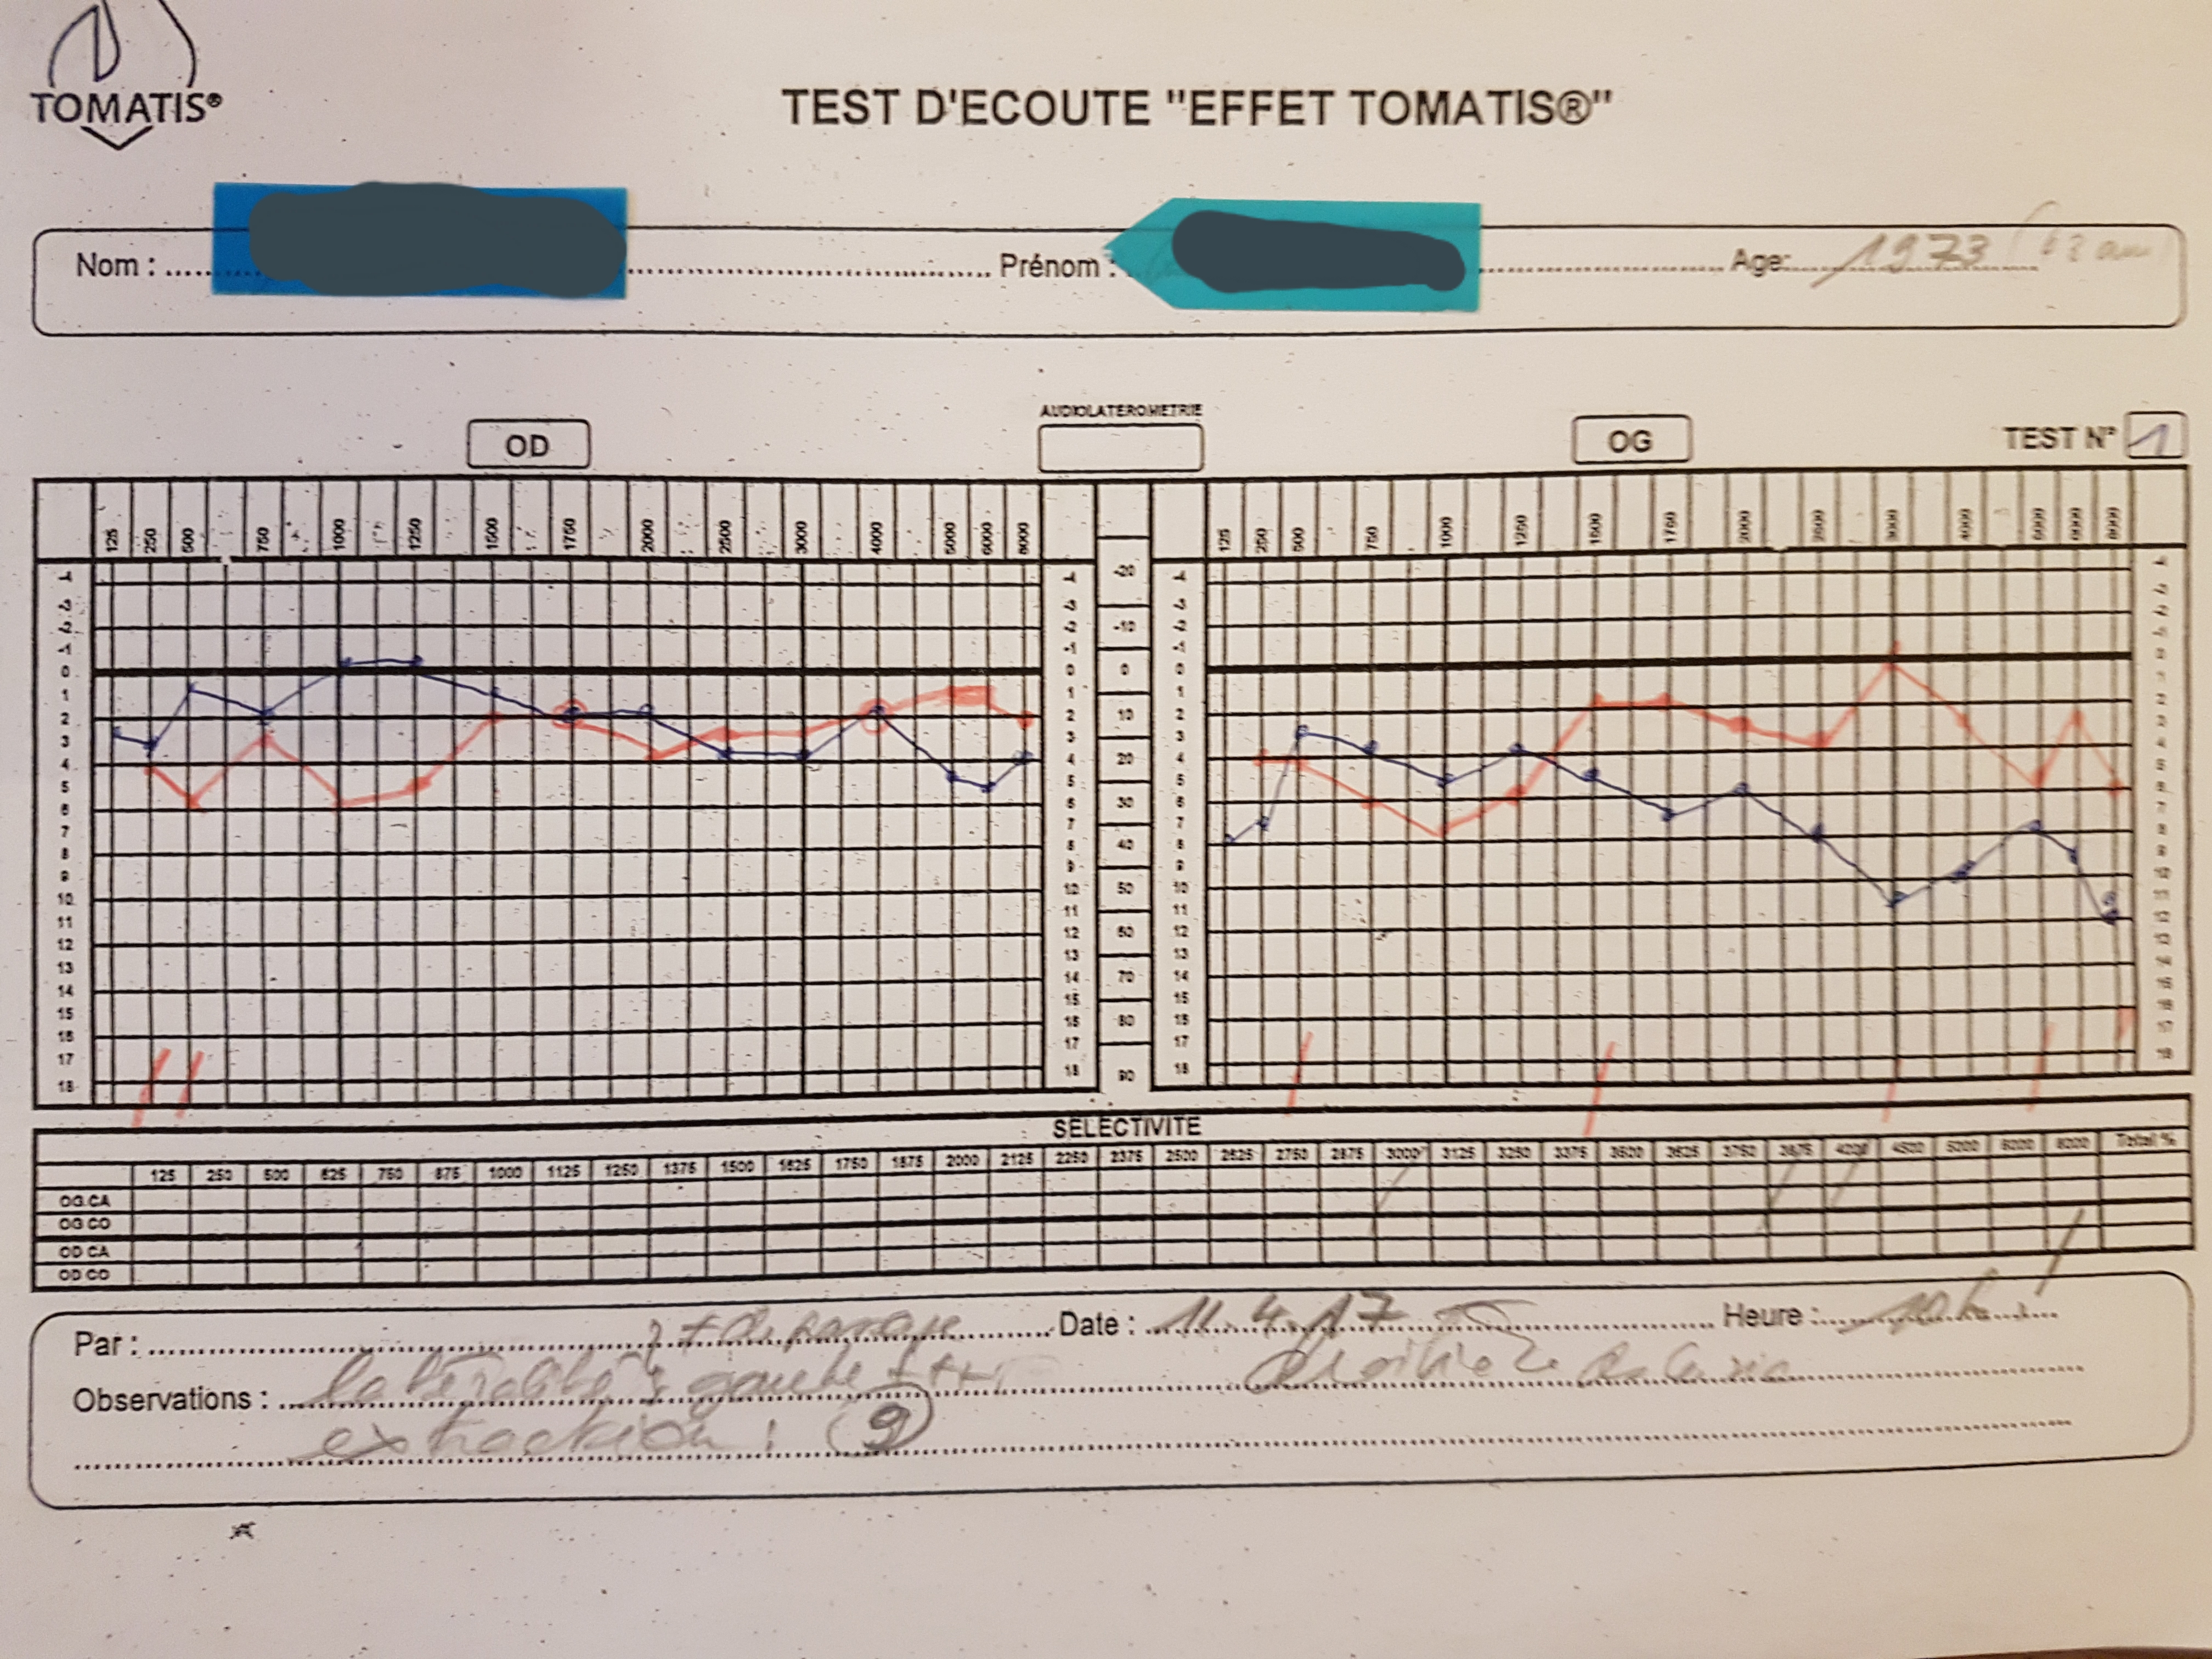
\includegraphics[width=0.7\linewidth]{images/courbesdeepressif.jpg}
	\caption{Courbes particulières d'un sujet diagnostiqué dépressif}
	\label{fig:courbes du dépressif}
      \end{figure}




      \paragraph{Descriptif selon les zones d'nterprétation:}

\begin{itemize}
  	\item Zone 1 :  Le rythme cardiaque: un stress intense va modifier le rythme
  du corps en augmentant ses fréquences. La respiration deviendra
  rapide. Il va s'en suivre une modification des perceptions
  extérieures. Une sensibilité particulièrement accrue aux bruits et
  aux sons peut en découler et être vécue comme une
  atteinte physique et psychique insupportable.
  Le changement de posture et d'attitude corporelle sont
notables (affaissement) et la perte d'énergie physique considérable (épuisement).
	\item Zone 2: La qualité de la voix: changement de la qualité du timbre de la
 voix et de l'émission verbale.	
  La voix se caractérise par son volume, son timbre, sa mélodie et son
  langage. Nous pouvons en faire le
        descriptif général, rejoignant ainsi l'idée émise lors du Congrès de la Société
américaine d'acoustique, de diagnostiquer la
        dépression par la voix:\footnote{Maryland University, 2004, 168\ieme\ Congrès de la Société
américaine d'acoustique.\autocite{le_service_metronews}. https://www.lci.fr/sante/et-si-on-diagnostiquait-la-depression-avec-u
n-test-vocal-sur-smartphone-1562728.html}.
          
 	\begin{enumerate}
 		\item le volume : basse intensité, faible dynamique
 		\item la mélodie : monotone, sans modulation
 		\item le timbre : mauvaise qualité due à une pertes des harmoniques
 		\item le langage : difficulté d'élocution, manque de fluidité
 	\end{enumerate}
        Il en découle une communication difficile avec l'entourage qui
        conduit au retrait social et à l'enfermement sur soi.
De même, un analyseur vocal peut permettre de suivre précisément l'amélioration de
l'identité vocale; sa visualisation conforte les progrès grâce aux
formants. L'enveloppe spectrale montre le timbre plus ou moins riche
dans l'empreinte vocale, renseignements précieux selon les cas.
        
	\item Zone 3: La confusion mentale, la démotivation, la perte d'énergie
psychique, la disharmonie intérieure/extérieure, le non-verbal.
\end{itemize}

 

 % \begin{figure}
%	\centering
%	\includegraphics[width=0.7\linewidth]{images/courbedepressif.jpg}
%	\caption[Exemple d'une courbe de dépressif]{Courbe
 %         représentative d'un dépressif, extrait de l'étude de Nantes,
   %      1987.}
       
%	\label{groupecontroleimage1}
%\end{figure}


	\textbf{Résonance des informations récoltées par les 3 
          zones du test d'écoute en musicothérapie et en
  psychologie :}
          
\begin{itemize}
 \item  Z.1: le physique, le corps, l'incorporation et
l'intégration du rythme,
la posture d'écoute  =  Rythme, tempo, puls 

\item  Z.2:  l'expression vocale, la communication,
l'émotionnel, la sensibilité, l'affect = Voix, timbre, mélodie 

\item Z.3: la créativité, l'interprétation, la
résonance, la musicalité, la motivation, le non-verbal (l'intraduisible en mot), l'espace = Justesse, harmonie (consonance,
dissonance), improvisation.
%\footnote{\{Hegi : L'improvisation joue un rôle centrale en musicothérapie (Hegi 1986)} 
\end{itemize}


Pour une optimalisation de l'écoute différenciée, il est souhaitable
de rejoindre dans un premier temps  le patient dans sa capacité
d'écoute de base, avec une adaptation et modulation consécutive du
volume sonore (seuils auditifs) et de l'utilisation de la voix (zone
2) en musicothérapie.
L'existence de difficultés de perception dans cette zone nous
induit à une meilleure compréhension et  élucidation de ces dernières à l'aide du
test d'écoute.

Pour élargir le concept de\textbf{ la zone 3,} comme on le
verra dans la rubrique des réflexions, nous pourrions 
également l'étendre aux notions winnicottiennes du jeu, de la capacité
créative dans un espace
intermédiaire, où l' \textit{``objet
transitionnel'' } (développé dans \textit{``Jeu et Réalité'',1953})
\autocite{winnicott} 
figure entre le ``le
dedans et le
dehors'',
l'interne et l'externe, et de là,  prolonger le questionnement du
rapport avec le concept des
courbes aérienne et osseuse.



Si on considère que ``\emph{l'alliage indissociable du corps et du psychisme, 
visible et lisible résulte de l'écoute de
sons'''}, \footnote{\emph{Extrait de l'entretien Tomatis réalisé par
  Auriol, Anvers 1973}} le concept de dépression ( R. Jouvent) \autocite{doronparot} (Cf. Annexes
A.5) inclut aussi l'idée d'une protection et une stratégie de
défense du psychisme, ayant un lien évident avec les zones du schéma d'écoute.

Même chez E.
Willems, \autocite{willems}, \footnote{  (dans sa \textit{Philosophie de la méthode} issu de sa
Pédagogie musicale) Copyright by Musique et Culture, Strasbourg} ,on relève des correspondances analogues entre les vies
corporelle (impulsions physiques)
---rythmique, affective (affection et sentiment) ---mélodique, mentale
(raisonnement et intellect)--- harmonique.


De plus, si nous nous référons à la conception indienne antique des chakras
ainsi qu'au sens de la seconde
topique de Freud (\textit{ça, moi et surmoi}), nous trouvons également des correspondances
entre les trois zones de 
fréquences et \textit{``la distribution de l'énergie pulsionnelle'}' ou entre
les 
\textit{``caractéristiques du son et l'énergie
instinctuelles''}\autocite[ch. 13]{auriol_cle_1996}.

\begin{figure}
	\centering
	\includegraphics[width=0.7\linewidth]{images/testinterpmusico}
	\caption[ L'interprétation des 3 zones et leur correspondance
        en musicothérapie]{Graphique: interprétation des 3 zones du
          test, leur correspondance en musicothérapie et selon les
          topiques de Freud.}
       
	\label{graphiquecolonnetestmusico}
      \end{figure}




%`\textit{`La mélodie est la seule forme musicale de la décharge individuelle,
%car le rythme est le moteur, pré-musical, et l'harmonie,
%supra-individuelle ``} (Mosonyi, 1835????, cité par Michel, 1965).


Ainsi, au lieu de séparer les trois grandes voies de la psychologie du
XXème siècle (psychanalyse, comportementalisme et pychologie
humaniste) comme nous le suggère T. Janssen
\autocite[197]{van_eersel_cerveau} il serait intéressant de les
considérer comme complémentaires.
%, comportant chacun un aspect qu'il
%nomme ``phénomène humain''.








      


  
 	
 	
 	
 
       
   
 





      



 











   
 

  

  
  


   
   
   
   







%\paragraph{Hypothèse}



%\paragraph{Y-a-t-il une modification de l'écoute du patient après une prise
%en charge en musicothérapie ?}
%Est-ce que le processus d'écoute en musicothérapie améliore la capacité
%d'écoute ? Devient-elle différente après une musicothérapie?

%Est-ce que les test auditifs avant et après la musicothérapie permettent
%de visualiser l'action de la musicothérapie?


%\paragraph{Est-ce que les résultats ($=$ un changement dans l'écoute) d'une prise
%en charge musicothérapeutique peuvent être lisibles et visibles dans
%un test d'écoute?}
%Est-ce possible d'évaluer un travail musicothérapeutique au moyen
%d'un test d'écoute?
%Est-ce que ces résultats sont significatifs? 

%\paragraph{Est-ce que l'écoute du patient s'est modifié ? si on a pu observer
%une modification, dans quel sens va -t-elle ?}

%Le contexte: 
%est-ce que le contexte est suffisant pour
%ressortir des résultats ?






\chapter{Hypothèse : Réflexions et interrogations}

\section{Evaluation du travail fait en musicothérapie : }

Apprendre à écouter, c'est un travail et des résultats peuvent être
visibles. Nous utilisons un outil qui est le son. Nous accompagnons
le patient d'un point A pour aller au point B : que s'est -il passé
dans son écoute? Nous pouvons apporter des résultats visibles et tangibles
d'une forme d'apprentissage de l'écoute, d'une transformation de la
perception.On se base sur un graphique résultant d'un test de reconnaissance
de sons qui permet de visualiser une transformation psychologique
de l'écoute. 
\begin{itemize}
\item Il y a des résultats : nous pouvons constater soit un changement,
un statisme, un apprentissage,ou un refus d'apprendre et de se transformer.
Ce sont des données qui peuvent servir à mieux comprendre le patient
et à l'accompagner dans son cheminement.
\begin{itemize}
	\item \textbf{La communication : }
	C'est un des points des plus importants : la relation est indispensable à créer pour toutes thérapies.
	Hypothèse : le test représente un cadre médical; celui-ci est perçu par beaucoup de patients comme étant rassurant ( l'effet de la blouse blanche); en dehors de cet aspect, ce cadre scientifique peut jouer dès cet instant déjà son rôle de soutien dans la prise en charge.
	Il y a une procédure très claire.
	D'autre part, le rôle du patient est différent dans son essence même, non pas dans le sens de "patere" souffrir et subir, mais valorisé dans celui du rôle actif qu'il peut jouer : celui-ci peut se rendre compte de sa capacité à influencer sa façon d'écouter, qu'il a une présence signifiante dans sa thérapie.  Il n'est pas passif. Bien sûr, cela peut paraître une évidence car on sait l'impact de la musique sur le corps tout entier. Mais ici on rejoint  le concept de musique intégrative déjà cité. ( cf.Vrait) Le patient peut être nourri par la musique mais n'est pas "passif" et seulement l'"objet " qui bénéficie du traitement musical. Son  écoute lui appartient en propre, elle est personnelle et modifiable. S'il y a modification, il peut y avoir un changement; et le mot "changement" prend alors une connotation différente,  le mouvement est y  sous-entendu,  une démarche peut en découler, voire une évolution. 
\end{itemize}


Est-ce utile à tout musicothérapeute d'avoir un appareil test d'écoute ? certainement pas. C'était un moyen de faire cette étude. Elle démontre par ailleurs  l'intérêt qu'il faut donner à la phase dite "active" chez Tomatis, qui est certainement  un de ses points faibles. La musicothérapie elle, est toujours active!
\item Des questions sous-jacentes peuvent émerger comme celles-ci :
\end{itemize}
\begin{enumerate}
\item Quelle est la part d' objectivité ? de subjectivité?
\item S'il n'y a pas de changement visible dans le test , quelles conclusions
peut-on en tirer ? le changement va-t-il toujours de pair avec le
patient? synchronisé ou différencié dans le temps?
\item Est-ce normatif? par cette démarche, il y a le risque de catégoriser
et de paralyser le patient dans son parcours. Mais, cela peut aussi
l'aider dans son travail, son évolution. Ces deux possibilités sont
intrinsèques à tous les tests.
\end{enumerate}
\begin{itemize}
\item Nous sommes confrontés de plus en plus à donner des rapports aux caisse-maladies.
S'il y a une constatation de changement, de progression, le résultat
n'enfermera pas le patient dans une catégorie psychologique, qui,
transmise à celles-ci, pourrait lui être négative pour la poursuite
de son cheminement professionnel, via la vie active. 
\item Est-ce que ce test pourrait être un outil pour les thérapeutes et
les patients ? 
\item Avoir un support réel, visible car graphique pourrait-il être d'une
quelconque utilité pour le patient et pour le thérapeute ?
\item Est-il possible, à partir de deux tests d'écoute, de tirer des hypothèses
sur l'impact du son, de la musicothérapie, du soin par le son, sur
un patient ?
\item Le patient reste au centre de nos préoccupations.
\item Serait-ce un moyen, une façon de démontrer par ce moyen simple (autre
que l'Irmfct) que représente le test d'écoute l'utilité de la musicothérapie
? et ainsi de permettre une plus large acceptation et diffusion de
ce type de thérapie dans plus de milieux hospitaliers ou autres ?


\end{itemize}

Comme l'exprime à juste titre André Malraux : ``\emph{Le monde de
	l'art n'est pas celui de l'immortalité , c'est celui de la métamorphose.''}
De même, la musique est un art produit par l'homme et qui a un impact
sur lui-même. Les deux interagissent, s'interpénètrent et s'auto-transforment
au cours des siècles. Ce que nous pourrons constater lors de l'aboutissement
d'une thérapie n'est pas de trouver une autre personne mais une transformation
de la perception de celle-ci par rapport au monde qui l'entoure. Selon
ce que nous vivons, nous nous transformons mais continuons à être
soi. Nous continuons à ``être soi'' mais autrement. Nous ne perdons
pas notre identité.

\section{La musicothérapie et la méthode Tomatis : }
La musicothérapie et la méthode Tomatis sont des concepts très différents. Bien que la notion d'écoute les réunit, bien que leur medium soit la musique et plus particulièrement le son, d'un côté il s'agit d'une thérapie et de l'autre, il s'agit d'une pédagogie, d'un entrainement de la musculature de l'oreille. 
Tomatis se focalise et opère essentiellement sur le capteur auditif (vestibulo-cochléaire) pour amener, par ce processus, le patient à une certaine  amélioration par rapport à sa vie actuelle, à des souhaits ou à des attentes précises; celle-ci peut se réaliser au niveau du langage et ce, par l'intermédiaire de la musique et du chant. Nous pouvons de notre côté  émettre l'hypothèse que si le contrôle auditif est de bonne qualité ainsi que l'émission vocale, c'est-à-dire que la boucle phono-auditive est élaborée sans problème, l'oreille est prête, même peut-être plus prête et apte à travailler beaucoup plus en profondeur avec tous les riches moyens que la musicothérapie propose.
Préparer le terrain, faire un travail physique de fond, un travail préparatoire de l'oreille pour que celle-ci soit totalement opérationnelle et prête à aborder un travail psychique. Voilà l'hypothèse énoncée et ce que nous nous pouvons conclure, en effet.
\appendix

\chapter{Acoustique}

\section{Courbe de Wegel}
\label{acoustique}

<<Effectivement la courbe de Wegel est la courbe de réponse obtenue
lorsque sont posées en abscisses les fréquences, et en ordonnées ascendantes
les intensités. Un premier seuil s'obtient, en partie basse, suivant
un minimum qui commence dans les fréquences graves à environ 
\SIrange{40}{50}{\dB}, avoisine ensuite la courbe des abscisses entre 2000 et \SI{3000}{\Hz}
et redevient ascendante à \SI{40}{\decibel} / \SI{50}{\decibel} dans les aigus entre \SI{8000}{\Hz} et
\SI{10000}{\Hz}. Cette courbe se complète et prend l'allure de citron selon
l'expression qu'on lui confère lorsqu'on envoie des
sons d'intensité croissante et qu'on obtient alors une courbe des
seuils maxima qui se déterminent là où l'oreille commence à souffrir,
d'où le nom de ``seuil de la douleur". Ces seuils
commencent dans les graves, également de \SIrange{50}{60}{\decibel}, rejoignant la première
courbe, puis ils atteignent \SIrange{120}{130}{\decibel} entre \SI{2000}{\Hz} et \SI{3000}{\Hz} pour
chuter ensuite dans les aigus en rejoignant également la première
courbe. La ligne médiane qui se situe aux environs de \SIrange{50}{60}{\dB}, qui
est linéaire représente une zone dite ``Zone de Munsen''.
Elle répond à la dynamique de l'oreille, c'est-à-dire
à sa zone ``optimale" de fonctionnement sans
distorsion. Dans toutes les autres zones, l'oreille
agit comme un filtre dont les pentes sont variables en fonction de
l'intensité, avec un lieu de rotation situé de \SIrange{1000}{2000}{\Hz}. Pour pallier ces distorsions toujours difficiles à intégrer
dans la lecture des schémas, les Américains ont standardisé les audiogrammes
du type de ceux que nous utilisons tous en inversant l'image
de Wegel et en redressant les \emph{minima} pour obtenir une ligne droite.
Ces normes gardent néanmoins une zone préférentielle de \SIrange{1000}{2000}{\Hz} malgré les compensations de \SIrange{30}{40}{\dB} accordées sur la courbe,
dans les graves et les aigus.>>
\autocite[Bernard Auriol, conversation, conférence]{auriol_stress}.

% OGA: stp la source bibliographique ou conférence

\section{Impédance}
\label{impedance}

Définition de l'impédance : L'impédance acoustique
caractérise la résistance qu'un milieu oppose à sa mise en mouvement
lorsqu'il est traversé par une onde acoustique. Elle est définie comme
le rapport de la pression acoustique sur la vitesse de déplacement
locale dans un milieu, et est généralement notée $Z$. Elle dépend de
la température. L'impédance caractéristique d'un milieu (solide, liquide
ou gazeux) est définie comme le rapport de la pression acoustique
sur la vitesse de déplacement en milieu ouvert (c'est-à-dire
en l'absence d'ondes réfléchies). L'impédance caractéristique est
une propriété du matériau considéré égale, dans le cas d'un espace
illimité, au produit de la masse volumique du matériau $\rho$
par la vitesse du son $c$ dans ce même matériau : $Z = \rho_{m} c$.

Unités : $\rho_{m}$ étant exprimé en \si{kg/m\cubed},
$c$ en \si{m/s}, $Z$ est
exprimé en \si{\pascal . s/m}.

\chapter{Feuille informative de l'étude faite à la Privatklinik von Meiringen}

\begin{german}

Information für Mitwirkende an der klinischen Studie
\foreignquote{german}{Evaluierung des aktiven Hörvermögens}


Sehr geehrte Damen und Herren,

Herzlichen Dank für Ihr Interesse an dieser Studie !

Wozu dient diese Studie und weshalb werden Sie um eine Teilnahme gebeten ?

Während Ihrem Klinikaufenthalt  in der Privatklinik von Meiringen werden Sie im Kontext 
unseres multidisziplinären Teams verschiedene Therapien besuchen, unter anderem auch die Musiktherapie. Bei der vorliegenden Studie möchten wir untersuchen, wie sich die Musiktherapie auf Ihr Zuhörvermögen auswirkt.
Musiktherapie ist eine gut erforschte Intervention im Bereich des Depressions und Burnouts, da Sie ein relativ neues Berufsfeld ist, gibt es noch viel Forschungspotential.
Das Hörtest konnte sich als ein Instrument erweisen, um die Veränderung des Gehörs des Patienten bei einer Musiktherapiebehandlung zu beweisen. Die Verbindung dieses Ansatzes mit der Musiktherapie ist noch nicht erforscht und daher soll dieser Ansatz wissenschaftlich näher untersucht werden.
Wenn Sie keine Musiktherapie besuchen aber Interesse für diese Studie haben, sind Sie herzlich eingeladen, dieses Test zu tun. Im Rahmen under MAS brauchen wir unbedingt eine Kontrollgruppe.

Wie sieht eine Teilnahme an der Studie aus ?

Die Untersuchung erfolgt sehr einfach in mehreren Schritten.
Zu Verfügung steht ein Apparat, mit dem sich spezifische Hörtests durchführen lassen.
Allgemein Verlauf des Tests :  
Sie hören einen sehr leisen Ton mit Zuhörern zu und werden ihn entweder mit der rechten  oder linken Hand  signalisieren. Das dauert ungefähr 30 Minuten.
Es wird zwei Tests geben : ein vor der Therapie und ein nach der Therapie.
Wir bitten Sie auch, eine kleine Fragebogen zu erfüllen.


Falls Sie Fragen haben, dürfen Sie sich gerne via E-Mail melden : valerie.gaillard\@gmx.ch

Wir bedanken uns herzlich für Ihre Zeit und die Teilnahme an dieser Studie.

\end{german}
Valérie Gaillard

\begin{french}
	Le matériel utilisé : une table, deux chaises, l'appareil
	test Hearing et les écouteurs aériens et osseux, un crayon, deux
	feutres (rouge et bleu), une feuille avec la grille de fréquences à
	remplir.
\end{french}
 

\textgerman{ZhdK : Upgrade MAS Klinische Musiktherapie 15-17}



\chapter{Questionnaires}

\includepdfmerge{French_WHOQOL-BREF.pdf, -, 
	WHOQOLALLEMANDBREFupdated.pdf, -}


%\section{Questionnaire 1}
%
%\includepdf[pages=-]{French_WHOQOL-BREF.pdf}
%
%\section{Questionnaire 2}
%
%\includepdf[pages=-]{WHOQOLALLEMANDBREFupdated.pdf}

\printglossary[title=Glossaire, toctitle=Glossaire]
%\selectlanguage{french}
%\nocite{*} % imprime toute la bibliographie et pas seulement
% les livres cités
\phantomsection
%\addcontentsline{toc}{chapter}{Bibliographie}
\label{bibliographie}
\printbibliography
\clearpage
\listoffigures
%\title{{*}}

%\maketitle
\begin{titlepage}
 \begin{center}
    \Large
    Déclaration de paternité\\





 Je soussignée, Valérie Gaillard, certifie avoir rédigé ce travail de mémoire sous ma propre responsabilité, de manière indépendante et sans aide extérieure.




 \vfill

 Genève et Grône, le 15 mai 2020.


 Valérie Gaillard
%  { \LARGE
%\emph{Le `` test d'écoute'' comme  révélateur de l'impact
%  du processus musicothérapeutique.}\\ \bigskip




	 \hfill \\
	 \rule{0mm}{0.5pt} \hfill
%{\large Zürich, juin 2020}
 \end{center}
\end{titlepage}

\end{document}

 Local Variables:
% TeX-engine: luatex End:
